\section{$t\bar{t}W$ process}
\label{sec:ttV}


\subsection{Samples}
Two MC generators are compared in this study.
The nominal sample for \ttW production was generated using the \textsc{Sherpa}~2.2.1~\cite{sherpa} generator with the NNPDF3.0 NLO PDF set. % and using the Meps\@NLO prescription with a merging scale of 30 GeV.
The matrix element (ME) was calculated for up to one additional parton at NLO and up to two partons at LO using
\textsc{Comix}~\cite{Gleisberg:2008fv} and \textsc{OpenLoops}~\cite{Cascioli:2011va}, and merged with the \textsc{Sherpa} parton shower~\cite{Schumann:2007mg} using the \textsc{MEPs@Nlo} prescription~\cite{Hoeche:2012yf} with a merging scale of 30 GeV.
The choice of renormalisation and factorisation scales is $\mu_R = \mu_F = H_\textrm{T}$/2, where $H_\textrm{T}$ is defined as the scalar sum of the transverse masses $\sqrt{p_\textrm{T}^2+m^2}$ of all final state particles.



Systematic uncertainties due to missing higher-order QCD corrections are estimated by varying the factorisation and renormalisation scales in the nominal sample simultaneously by a factor of 0.5 (2.0) with respect to the central value called further SherpaScaleDown (SherpaScaleUp). % ($\mu_R=\mu_F=0.5$ and $\mu_R=\mu_F=2.0$ ). 
Uncertainties associated with the modelling of additional QCD radiation are estimated by comparing the nominal \ttW prediction with that of an alternative sample that was generated at NLO with the \textsc{MadGraph5\_aMC@NLO}~2.2.1 (MG5\_aMcAtNlo) generator using the same scale choice and PDF set as for the nominal sample, and interfaced to \textsc{Pythia}~8.2 in combination with the A14 tune. 
The samples configurations are summarised in Table~\ref{tab:mcconfig}.
%%%%%%%%%%%%%%%%%%%%%%%%%%%%%%%%%%%%%%%%
\begin{table}
\begin{center}
\caption{\label{tab:mcconfig}
The configurations used for the event generation of the \ttW processes.}
\vspace{0.25cm}
{\small
\setlength\tabcolsep{1.5pt}
\begin{tabular}{llllll}
\hline\hline
Process & Generator & ME order & Parton shower & PDF & Tune  \\
%& (alternative) & (alternative) & & \\
\hline
$\ttbar W$  & \textsc{Sherpa 2.2.1} & \textsc{MePs@Nlo} 0,1@NLO+2,3@LO & \textsc{Sherpa} &  NNPDF3.0 NNLO & \textsc{Sherpa} default \\
& \textsc{MG5\_aMcAtNlo} & NLO & \textsc{Pythia} 8 & NNPDF3.0 NLO & A14   \\
\hline\hline
\end{tabular}
}
\end{center}
\end{table}


% Finally, the uncertainty due to the choice of PDF set is evaluated using the PDF4LHC15 prescription.

\subsection{Fiducial Volume}
\label{sec:ttw_fid}
Object and event selection is defined at particle-level that closely matches the detector-level described in reference~\cite{ATLAS-CONF-2019-045} and was defined together with CMS as a common phase space. 
Jets are reconstructed from stable particles with a mean lifetime of $\tau > 3\times 10^{-11}$~s, using the anti-$k_t$ algorithm with a radius parameter of $R=0.4$.
Jets are required to satisfy \pt > 25 GeV and $|\eta|$ < 2.5.
Jets that are matched to $b$-hadrons with \pt>5 GeV by ghost matching~\cite{Cacciari:2008gn} are referred to as $b$-jets. 
Electrons and muons, referred to as light leptons $\ell$, are required to be separated from selected jets by $\Delta R>0.4$ and are otherwise removed. 
Hadronically decaying $\tau$ leptons are required to satisfy \pt> 25 GeV and $|\eta| $< 2.5.
Events are selected with exactly two light leptons.
Leptons are required to have $|\eta|$< 2.5 and \pt>25(20) GeV for leading $\ell_0$ (subleading $\ell_1$) lepton (\pt ordered). 
Leptons are required to have same charge, targeting the semi-leptonic $\mathrm{t\bar{t}}$ decay and leptonic $W$ decay.

%Events separated by Hadronic tau decays Hadronically decaying $\tau$ lepton
Events with at least 3 jets and at least one of them being a $b$-jet are considered in the fiducial volume. 
%Events with at least 3 jets and least one $b$-jet are considered in the fiducial volume. 
The acceptance for events passing this selection is $A_X^{\geq1b\geq3j}=1.82\times10^{-2}$ for \textsc{Sherpa} and 1.90$\times10^{-2}$ for \textsc{MadGraph5\_aMC@NLO} correspondingly.
We then split into five regions, categorized by the number of jets of any flavour (three or  $\geq$4), $N_{b-\mathrm{jets}}$ (one or $\geq$2) as well as the presence of hadronically decaying $\tau$ lepton, as summarised in Table~\ref{tab:ttWregions}.

\begin{table}
\begin{center}
\caption{\label{tab:ttWregions}
The configurations used for the event generation of the \ttW processes.}
\vspace{0.25cm}
{\small
\setlength\tabcolsep{1.5pt}
\begin{tabular}{l|l}
\hline\hline
Region & Selection  \\
%& (alternative) & (alternative) & & \\
\hline
1  & $N_{b-\mathrm{jets}}=$1, $N_{\mathrm{jets}}\geq$4 , 0-$\tau_{had}$ \\
2 & $N_{b-\mathrm{jets}}\geq$2,   $N_{\mathrm{jets}}\geq$4, 0-$\tau_{had}$ \\
3 & $N_{b-\mathrm{jets}}=$1,  $N_{\mathrm{jets}}$=3 , 0-$\tau_{had}$ \\
4 & $N_{b-\mathrm{jets}}\geq$2, $N_{\mathrm{jets}}$=3, 0-$\tau_{had}$ \\
5 & $N_{b-\mathrm{jets}}\geq$1, $N_{\mathrm{jets}}\geq$3 , 1-$\tau_{had}$\\

\hline
\hline
\end{tabular}
}
\end{center}
\end{table}

The definitions of the regions are motivated by the $t\bar{t}H$ Multilepton analysis strategy.
Regions 1 and 2 corresponds to the signal regions\footnote{slightly different then in ref.~\cite{ATLAS-CONF-2019-045}, in order to define a common selection with the CMS Collaboration.} and Regions 3 and 4 are used as control regions in the 2$\ell$ same-sign  0-$\tau_{had}$ $t\bar{t}H$ channel.
Definition of Region 5 is closely followed\footnote{requirement on jet multiplicity is relaxed.} by the selections in the 2$\ell$ same-sign 1-$\tau_{had}$ $t\bar{t}H$ channel.

%The event selection requirements are summarized in Table~\ref{}.
%defined by 5 jets \& 3 b-jets or >=6jets \& >=4 b-jets.




\subsection{Results}
%$N_{jets}$, $N_{b-jets}$,  $HT^{\text{jets}}$, leading $b$-jet $p_T$ Leading lepton $p_T$, $|\Delta \phi _{\ell \ell }|$, $\Delta R _{\ell \ell }$, $max |\eta _l|$
\begin{table}[]
\begin{center}
\caption{\label{tab:ttw_varlist}
The list of the validation variables for the comparison of the \ttW generators. The leptons $\ell$ and $b$-jets are ordered in \pt - leading correspond to highest \pt. }
\vspace{0.25cm}
{\small
\setlength\tabcolsep{1.5pt}
\begin{tabular}{l|l|c}
\hline\hline
Variable & Description & Regions \\ \hline
$N_{jets}$   &     Jet multiplicity        &      1,2,5   \\ %\hline
 $N_{b-jets}$       &     Number of  $b$-jets       &   1,2,5      \\ %\hline
$HT^{\text{jets}}$      & Scalar sum of transverse momentum of all jets in the event         &  1,2,3,4       \\ %\hline
$p_T^{b0}$       &      Leading $b$-jet transverse momentum       &   1,2      \\ %\hline
 $p_T^{\ell 0}$      &   Leading lepton transverse momentum           &     1,2,5    \\ %\hline
$\Delta R _{ \ell 0\mathrm{jets} }$      &     Minimum angular separation between the leading lepton and the nearest jet         &  1,2       \\ %\hline
$\Delta R _{\ell 0\ell1 }$      &       Angular distance between the two leptons      &    1,2,5    \\ %\hline
$max |\eta _l|$      &    Value of the highest lepton's pseudorapidity in the event        &     1,2    \\ %\hline
    $|\Delta \phi _{\ell \ell }|$    &    Azimuthal separation between the leptons         & 1,2    \\
    \hline\hline    
\end{tabular}
}
\end{center}
\end{table}

%Distribution of the angular distance between the two leptons (top), maximum between lepton $|\eta_{\ell 0}|$ and $|\eta_{\ell 1}|$ (centre), azimuthal separation between the leptons $\Delta \phi _{\ell \ell }$ (bottom) , for the Region 1 with 1$b$-jet (left) and Region 2 with 2$b$-jets (right) selection requiring four and more jets. 

The nominal  \textsc{Sherpa} \ttW  sample is compared to its radiation uncertainty variations and the alternative generator.
The ratio plots show the ratios of the alternative MC sample and scale variation to the nominal sample.

The list of variables for the comparison of the \ttW generators presented in this note are summarised in Table~\ref{tab:ttw_varlist}.
Two sets of distributions are presented: the first comparing the shapes of the different generators - distributions are normalised to the integral, the second - comparing overall generator agreement - distributions are scaled to the cross section used at generation. % (taken directly from generation - i.e. not including any correction factors).

\subsubsection{Shape comparison}
\label{sec:ttw_shape}
In the following shape agreement between nominal and alternative generators will be presented - distributions are normalised to the integral.
%$N_{b-\mathrm{jets}}=$

Sizeable discrepancies in the modelling of jet kinematics can be seen between the \textsc{Sherpa} \ttW and \textsc{MadGraph5\_aMC@NLO} generators in the $N_{b-\mathrm{jets}}$=1 regions, while in the $N_{b-\mathrm{jets}}\geq$2 regions the difference is reduced, as illustrated in Figures~\ref{ttV:4j12b} and~\ref{ttV:3j12b} for the high (Regions 1 and 2) and low (Regions 3 and 4) jet multiplicities correspondingly. 
Differences in distributions of $b$-jet kinematics follow a similar trend - sizeable discrepancies in the $N_{b-\mathrm{jets}}$=1 regions and agreement within scale uncertainties in the $N_{b-\mathrm{jets}}\geq$2 regions, as presented on Figures~\ref{ttV:4jbinfo} for Regions 1 and 2.


\begin{figure}[!htb]
\centering
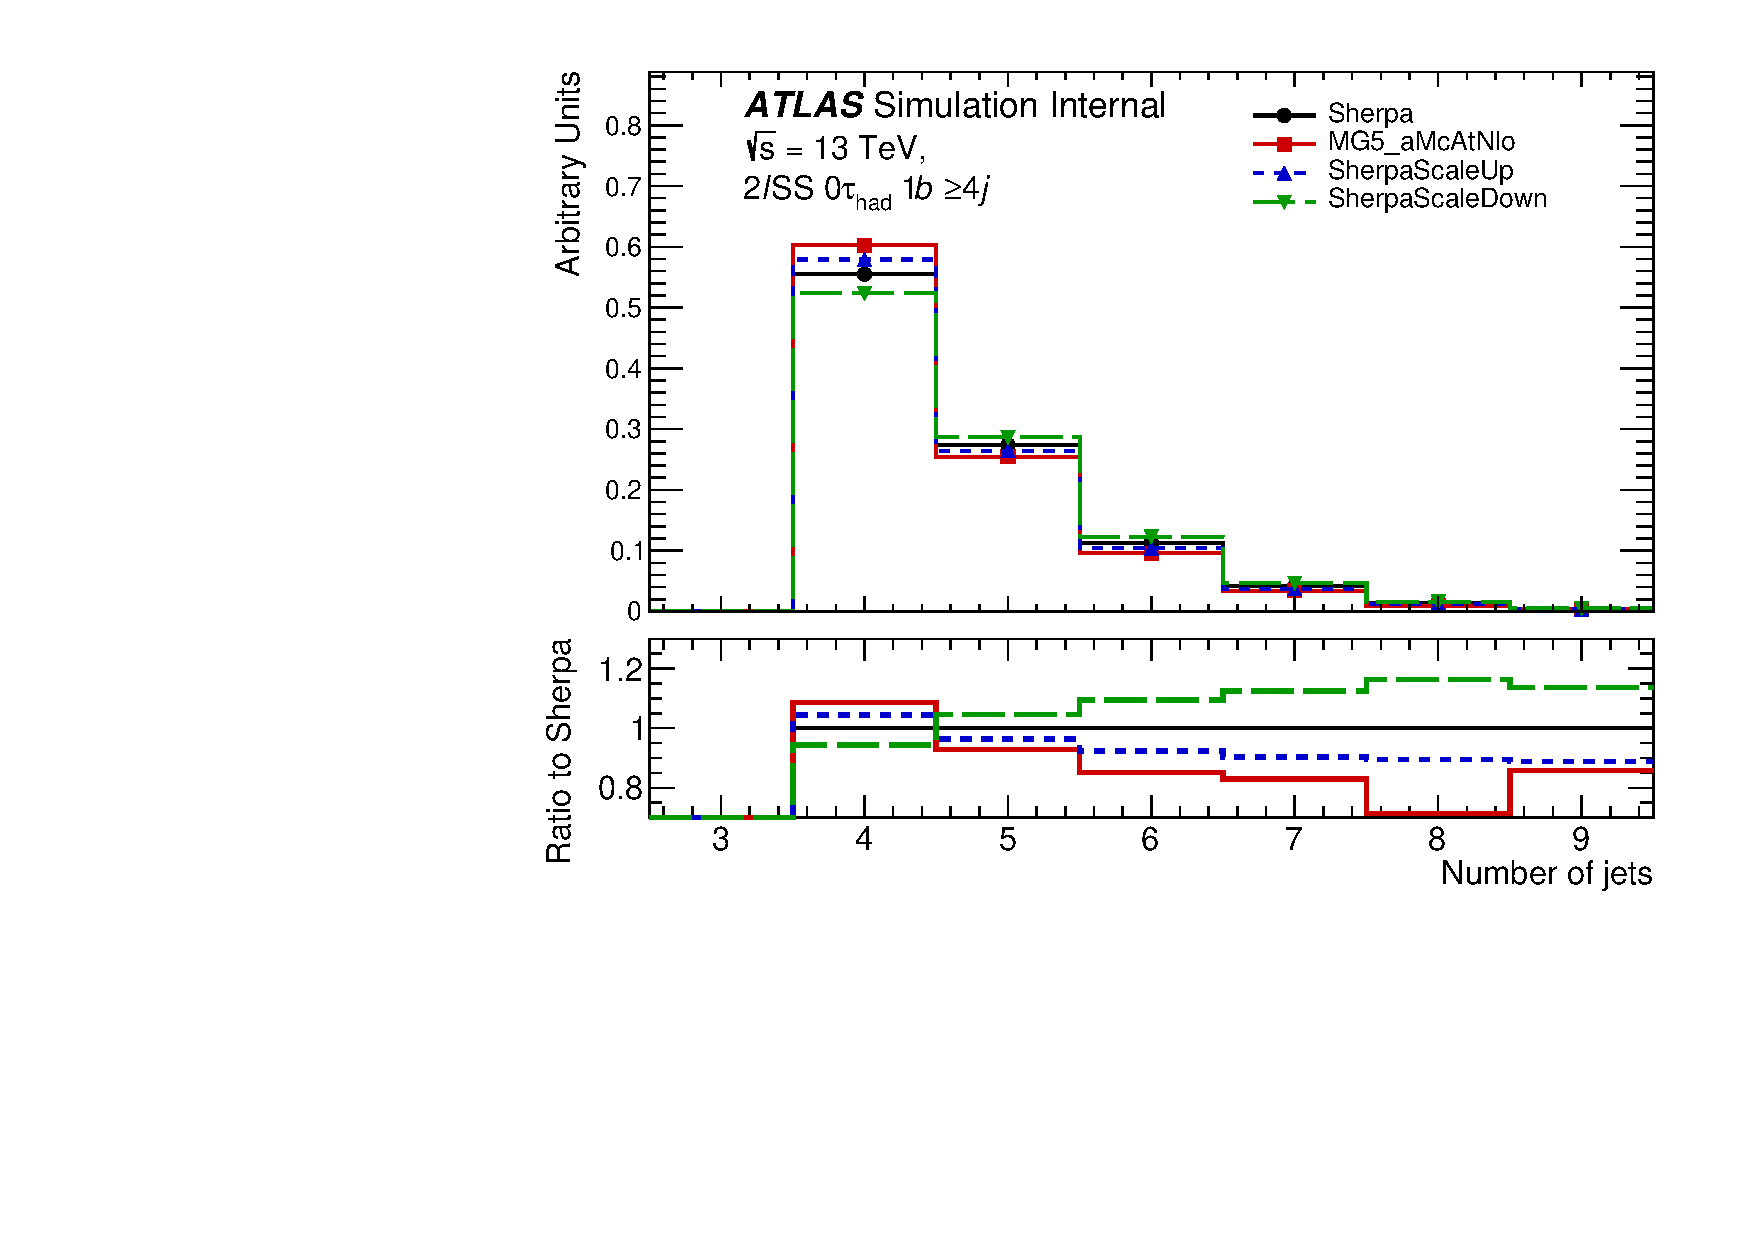
\includegraphics[width=0.45\textwidth]{Plots/ttV/shape/c_Region_0_nJets}
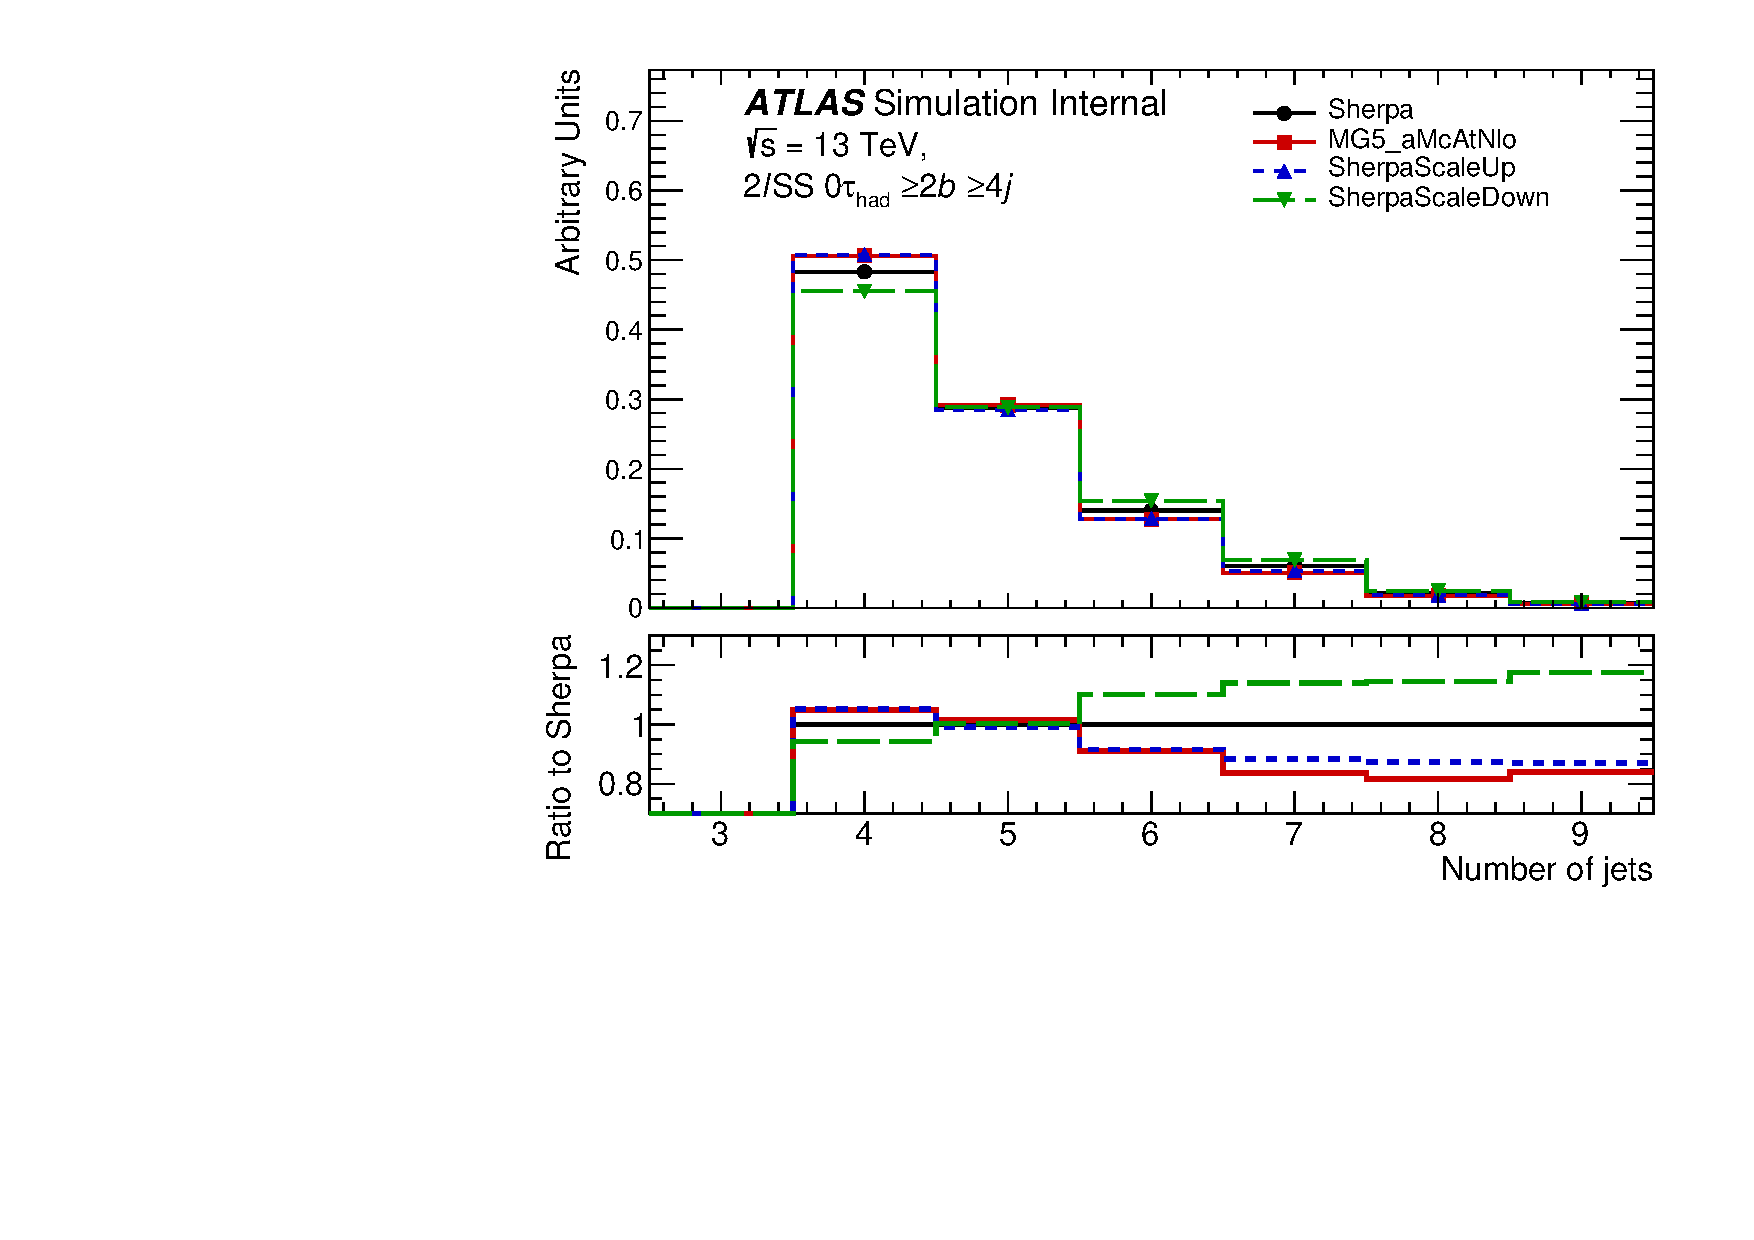
\includegraphics[width=0.45\textwidth]{Plots/ttV/shape/c_Region_1_nJets}\\
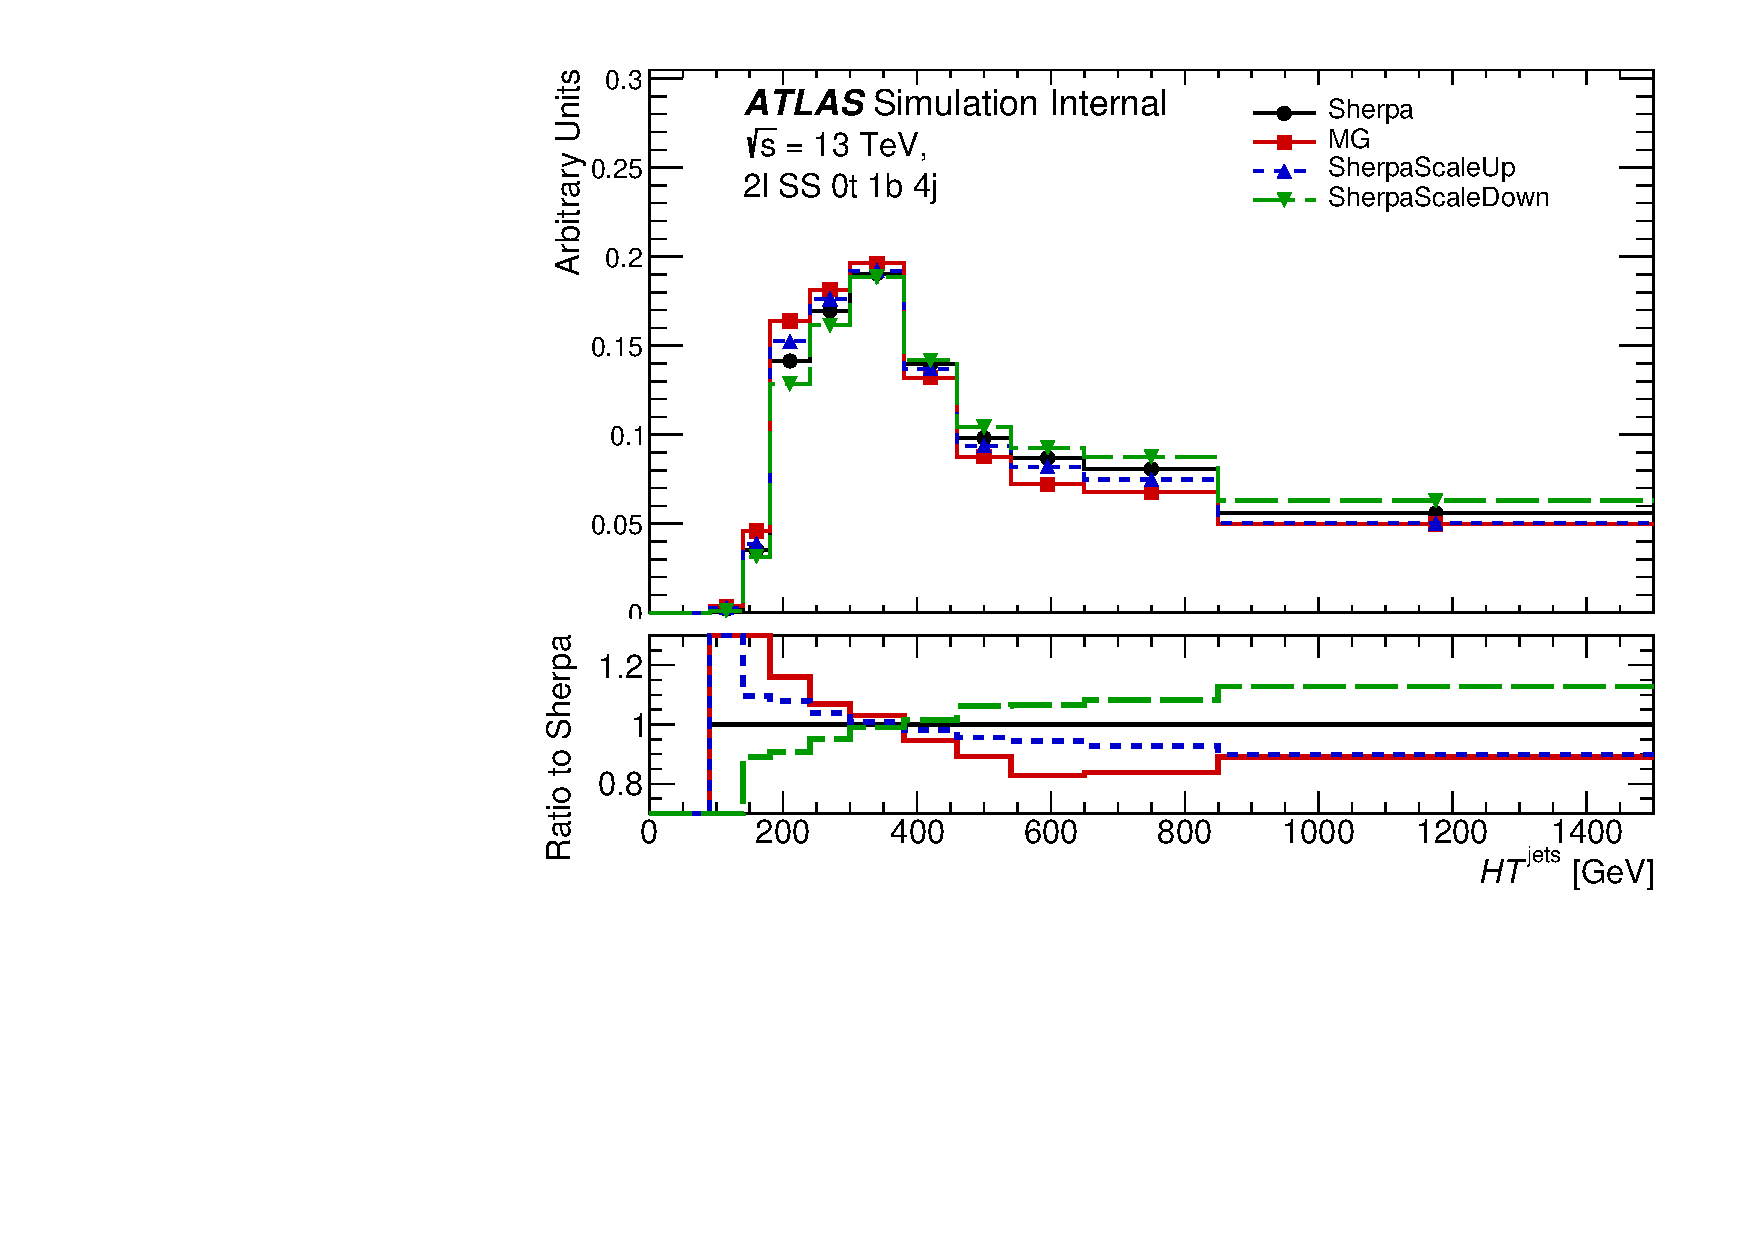
\includegraphics[width=0.45\textwidth]{Plots/ttV/shape/c_Region_0_HT_jets}
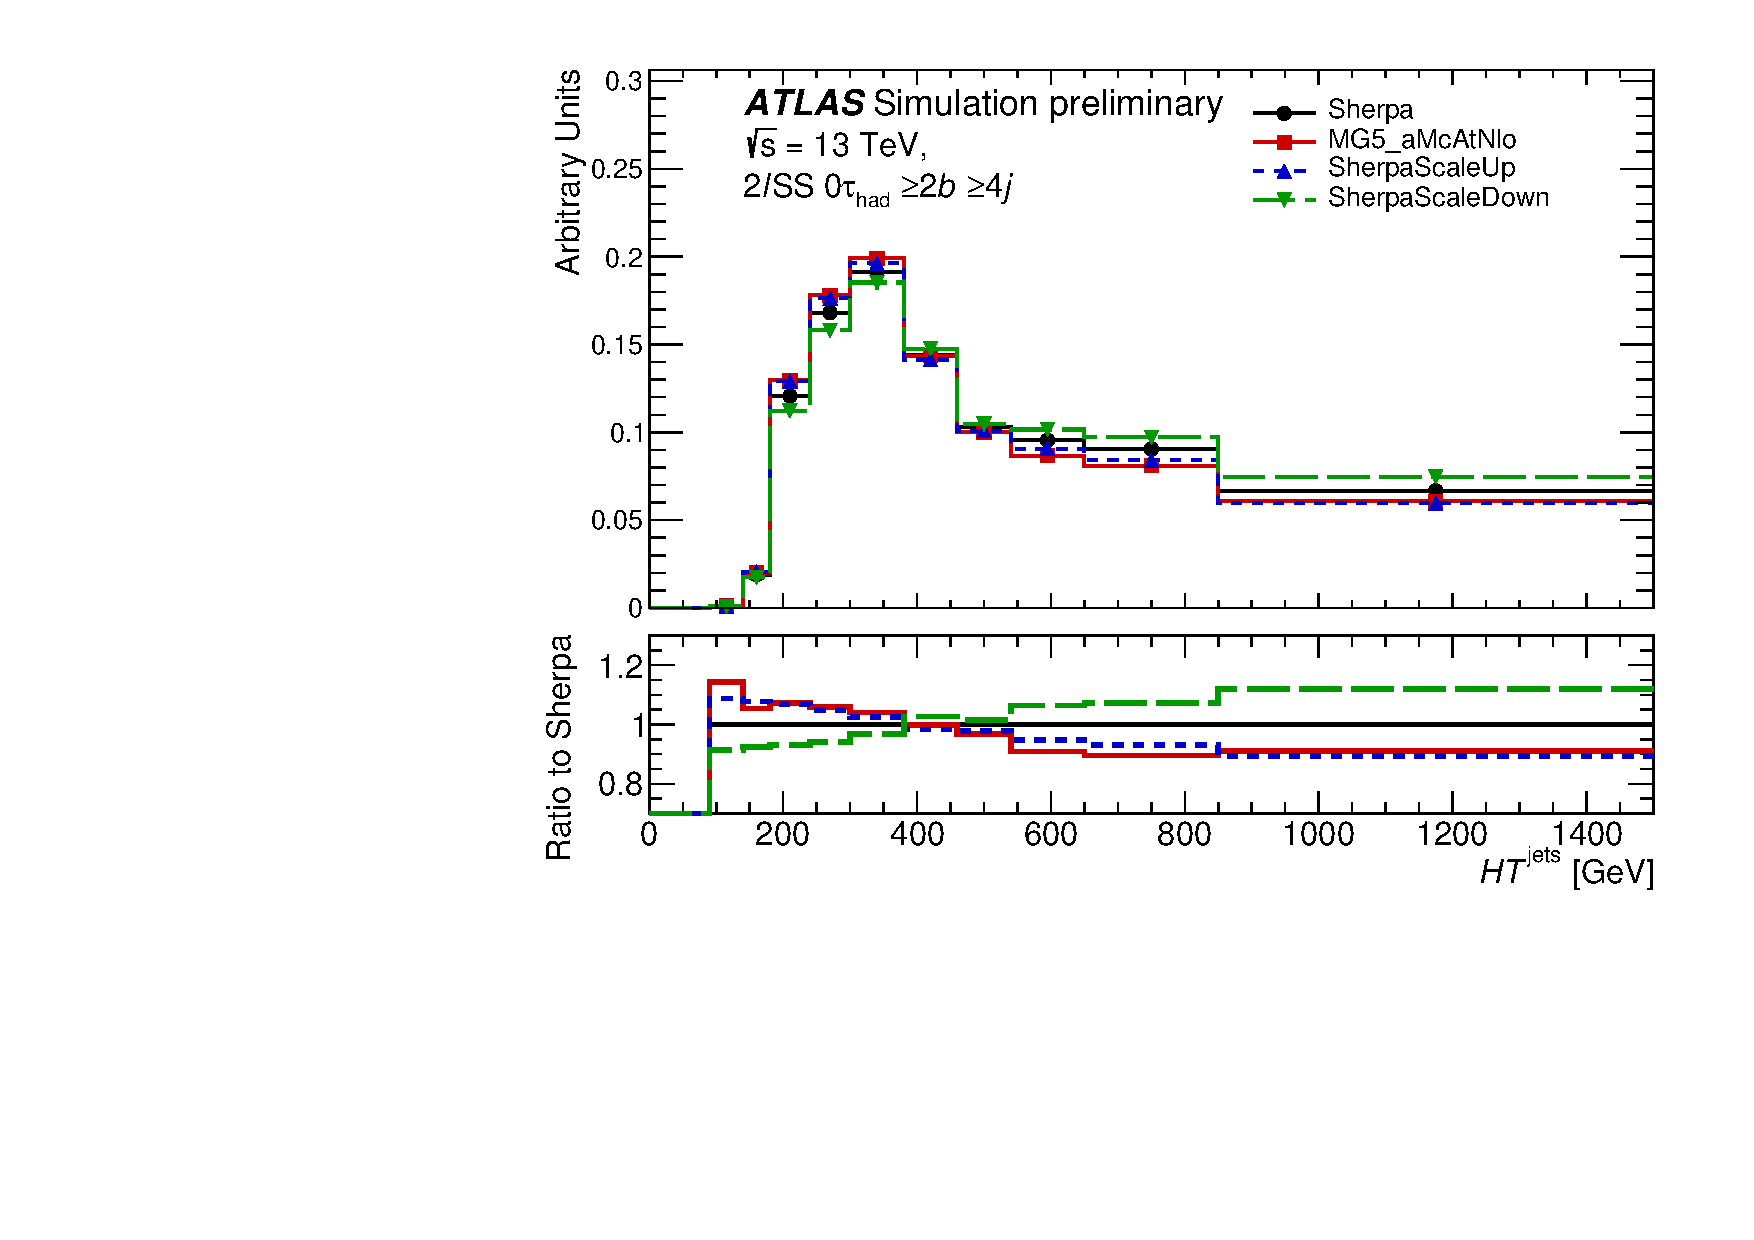
\includegraphics[width=0.45\textwidth]{Plots/ttV/shape/c_Region_1_HT_jets}\\
  \caption{Distribution of the jet multiplicities (top) and the scalar sum of jets transverse momentum, $HT^{\text{jets}}$ (bottom), for the Region 1 with $N_{b-\mathrm{jets}}=$1 (left) and Region 2 with  $N_{b-\mathrm{jets}}\geq$2 (right) selection requiring four and more jets.  \label{ttV:4j12b}}
\end{figure}


\begin{figure}[!htb]
\centering
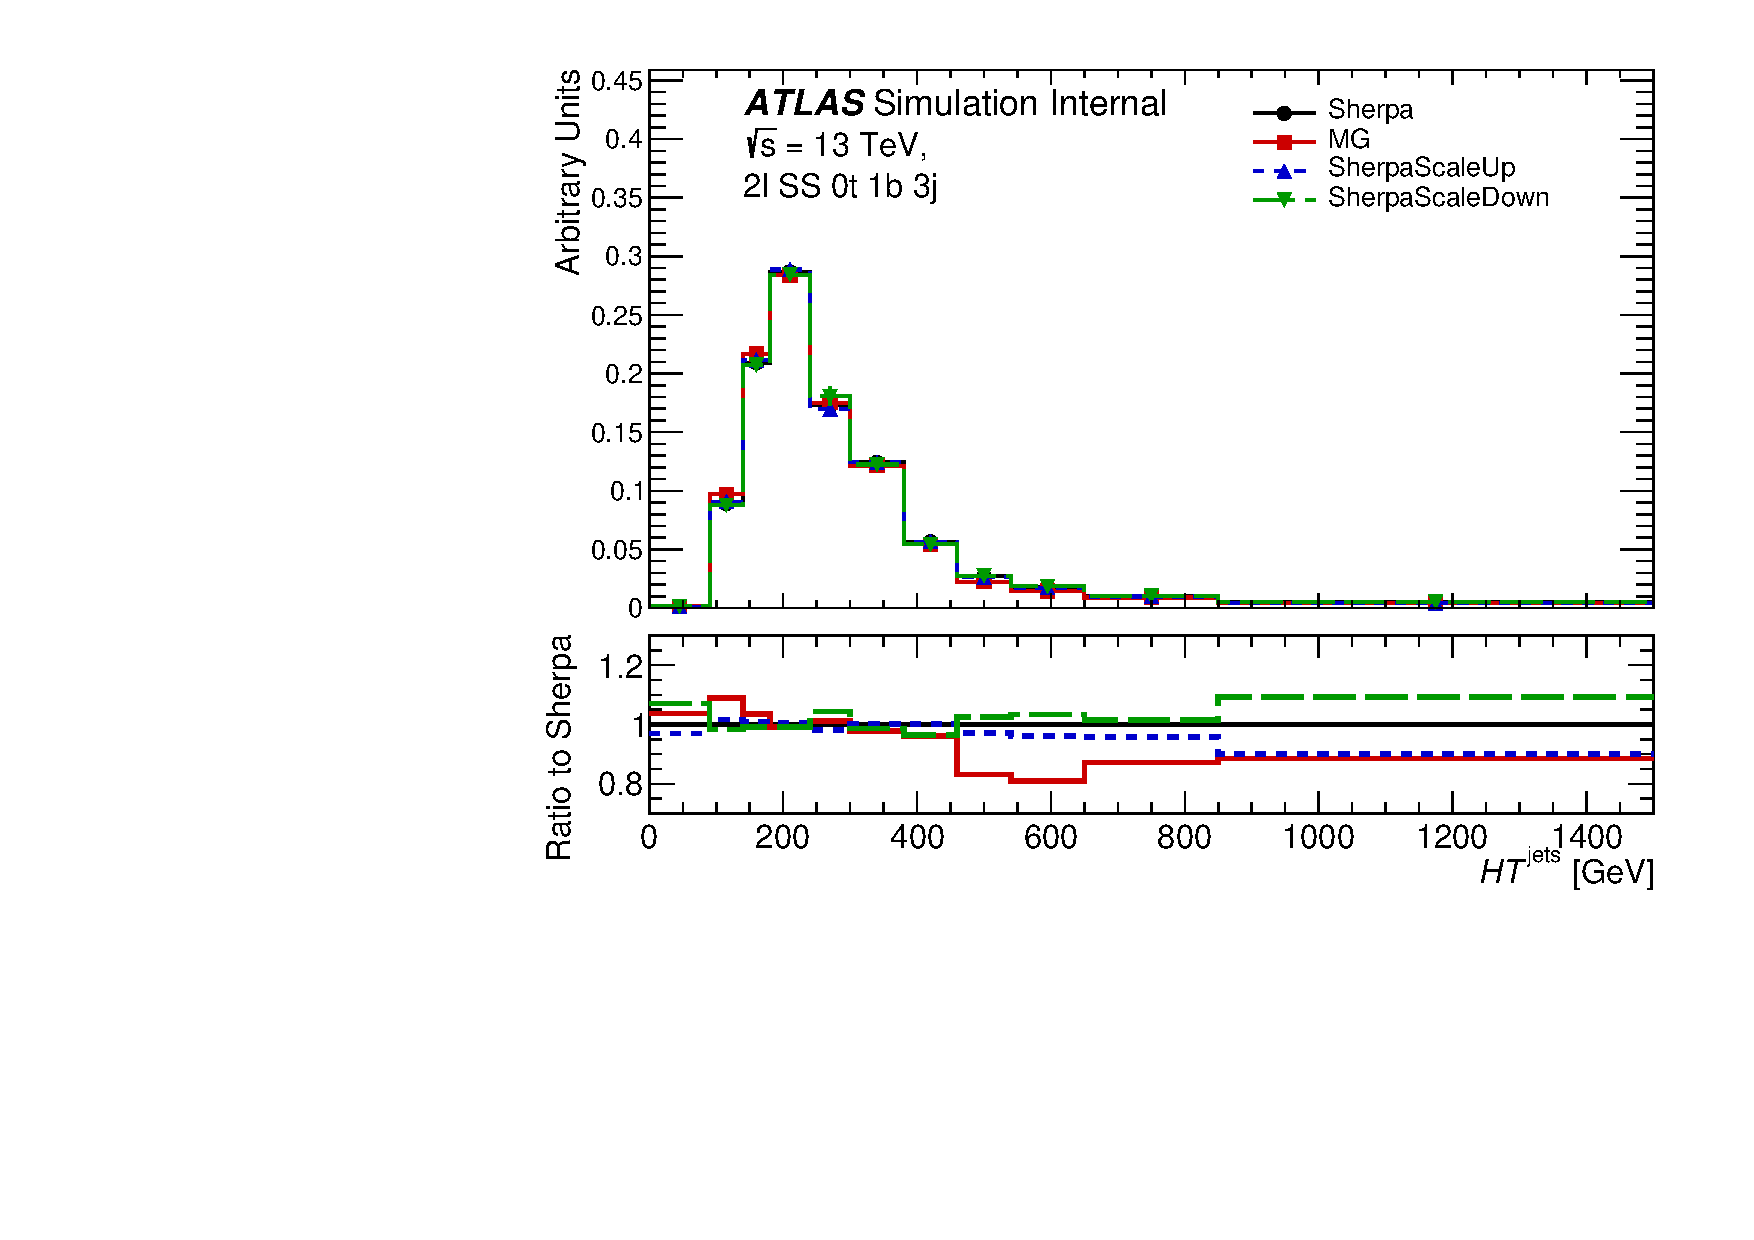
\includegraphics[width=0.45\textwidth]{Plots/ttV/shape/c_Region_2_HT_jets}
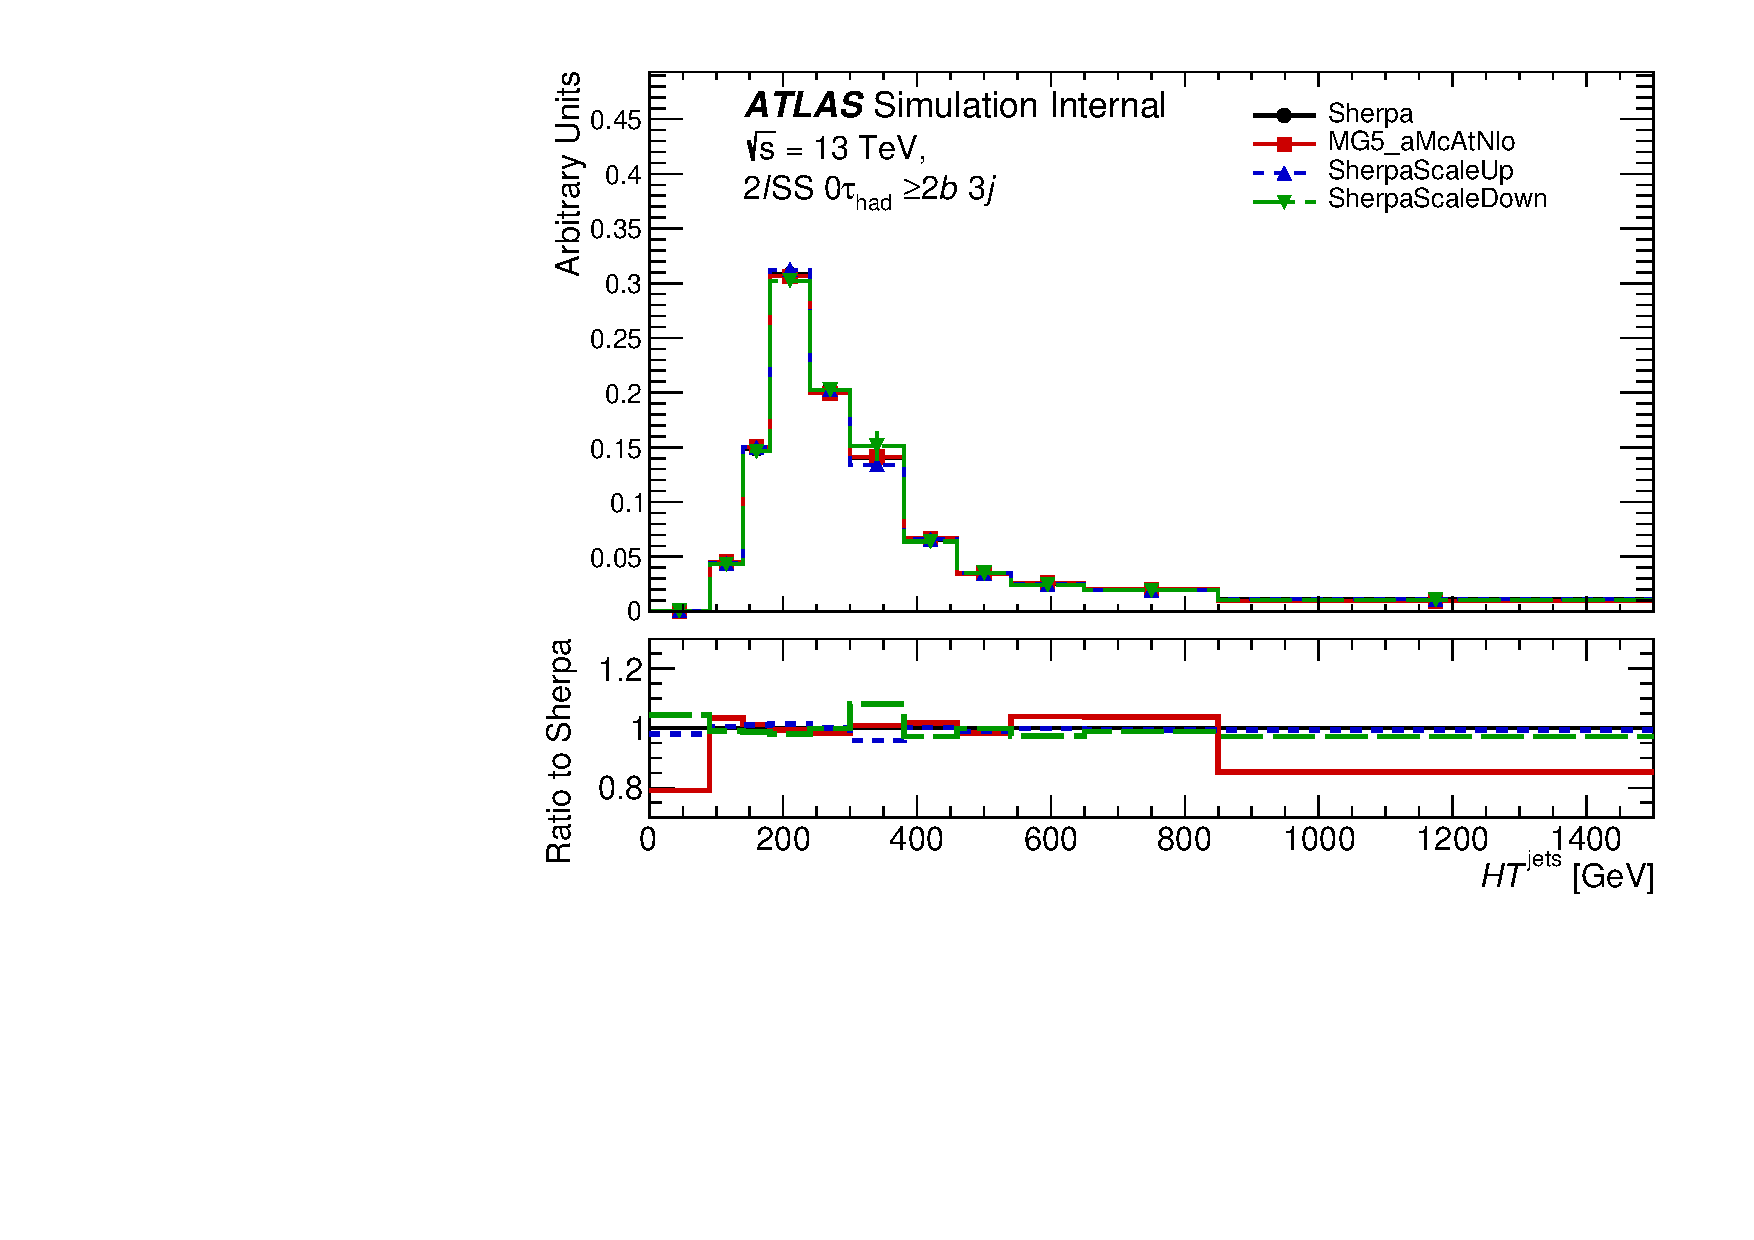
\includegraphics[width=0.45\textwidth]{Plots/ttV/shape/c_Region_3_HT_jets}\\
  \caption{Distribution of the scalar sum of jets transverse momentum, $HT^{\text{jets}}$, for the Region 3 $N_{b-\mathrm{jets}}$ = 1 (left) and Region 4 with $N_{b-\mathrm{jets}}\geq$2 (right) selection requiring exactly three jets.  \label{ttV:3j12b}}
\end{figure}


\begin{figure}[!htb]
\centering
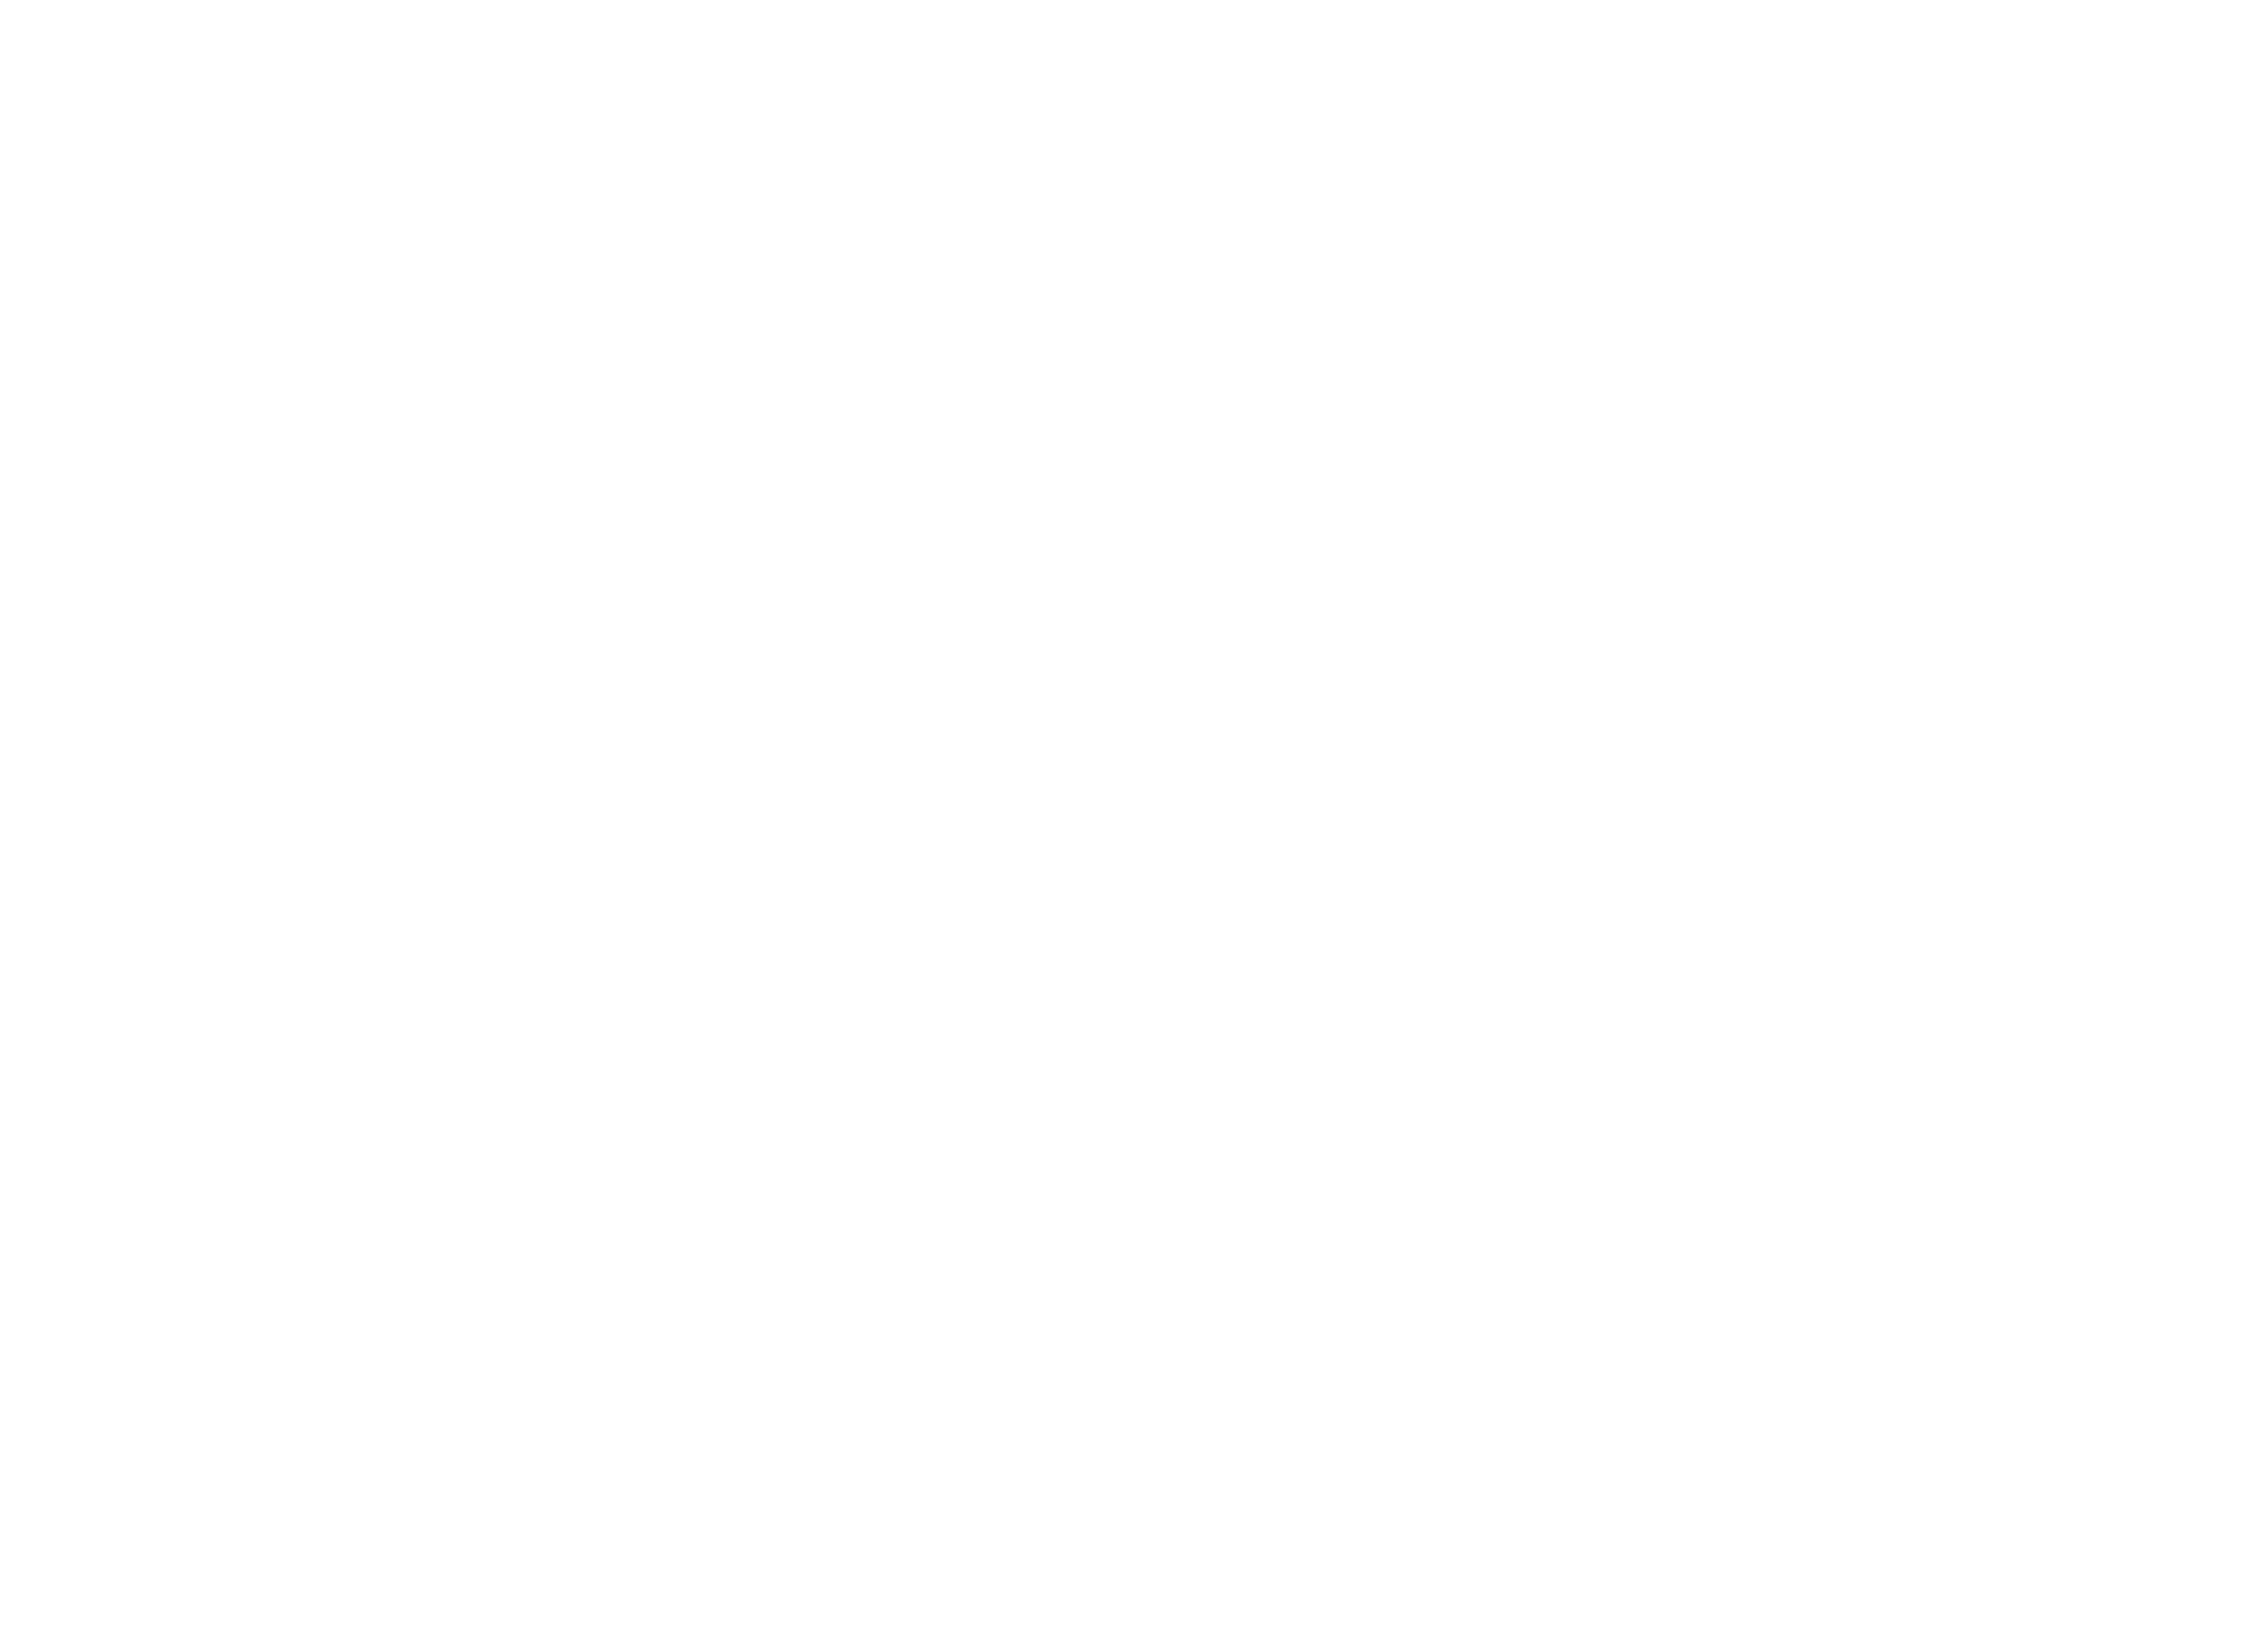
\includegraphics[width=0.45\textwidth]{Plots/ttV/dummy}
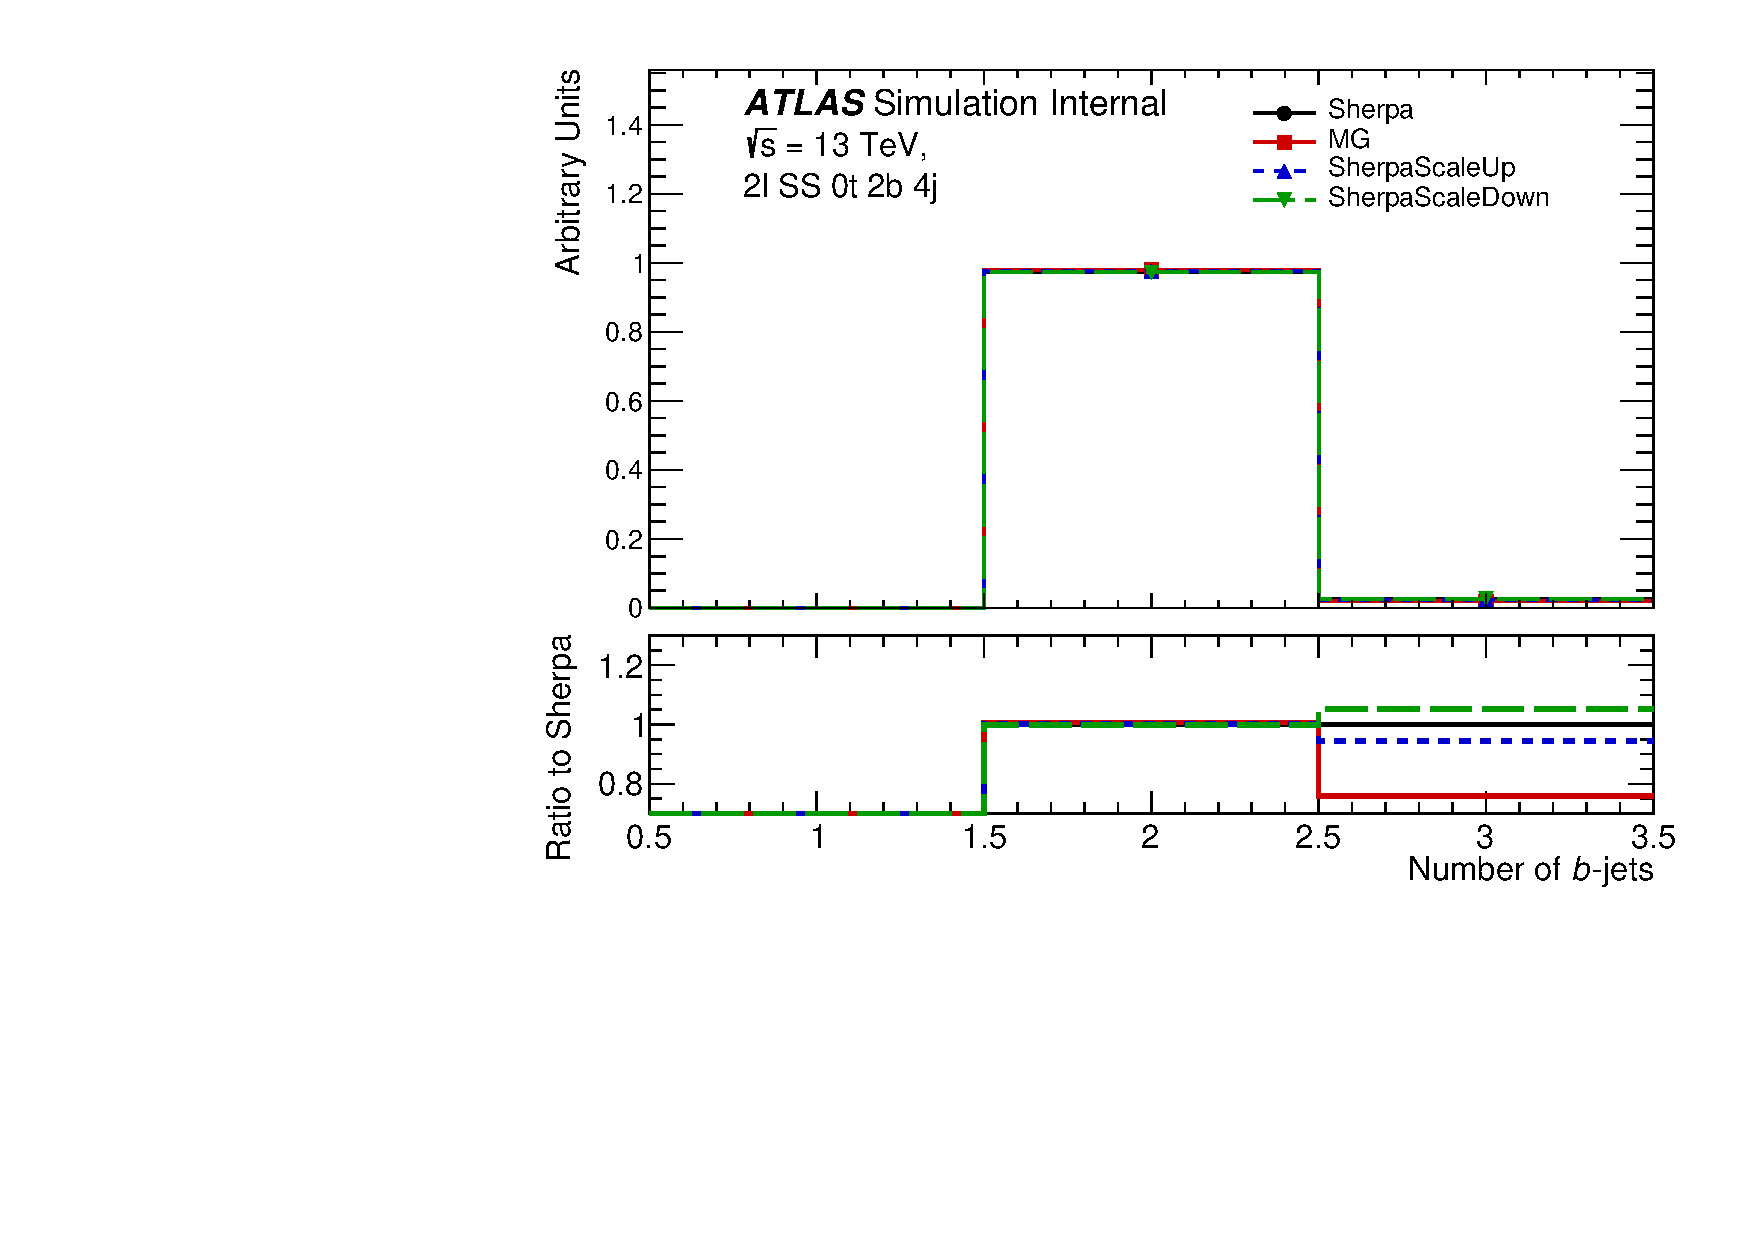
\includegraphics[width=0.45\textwidth]{Plots/ttV/shape/c_Region_1_nBtagJets}\\
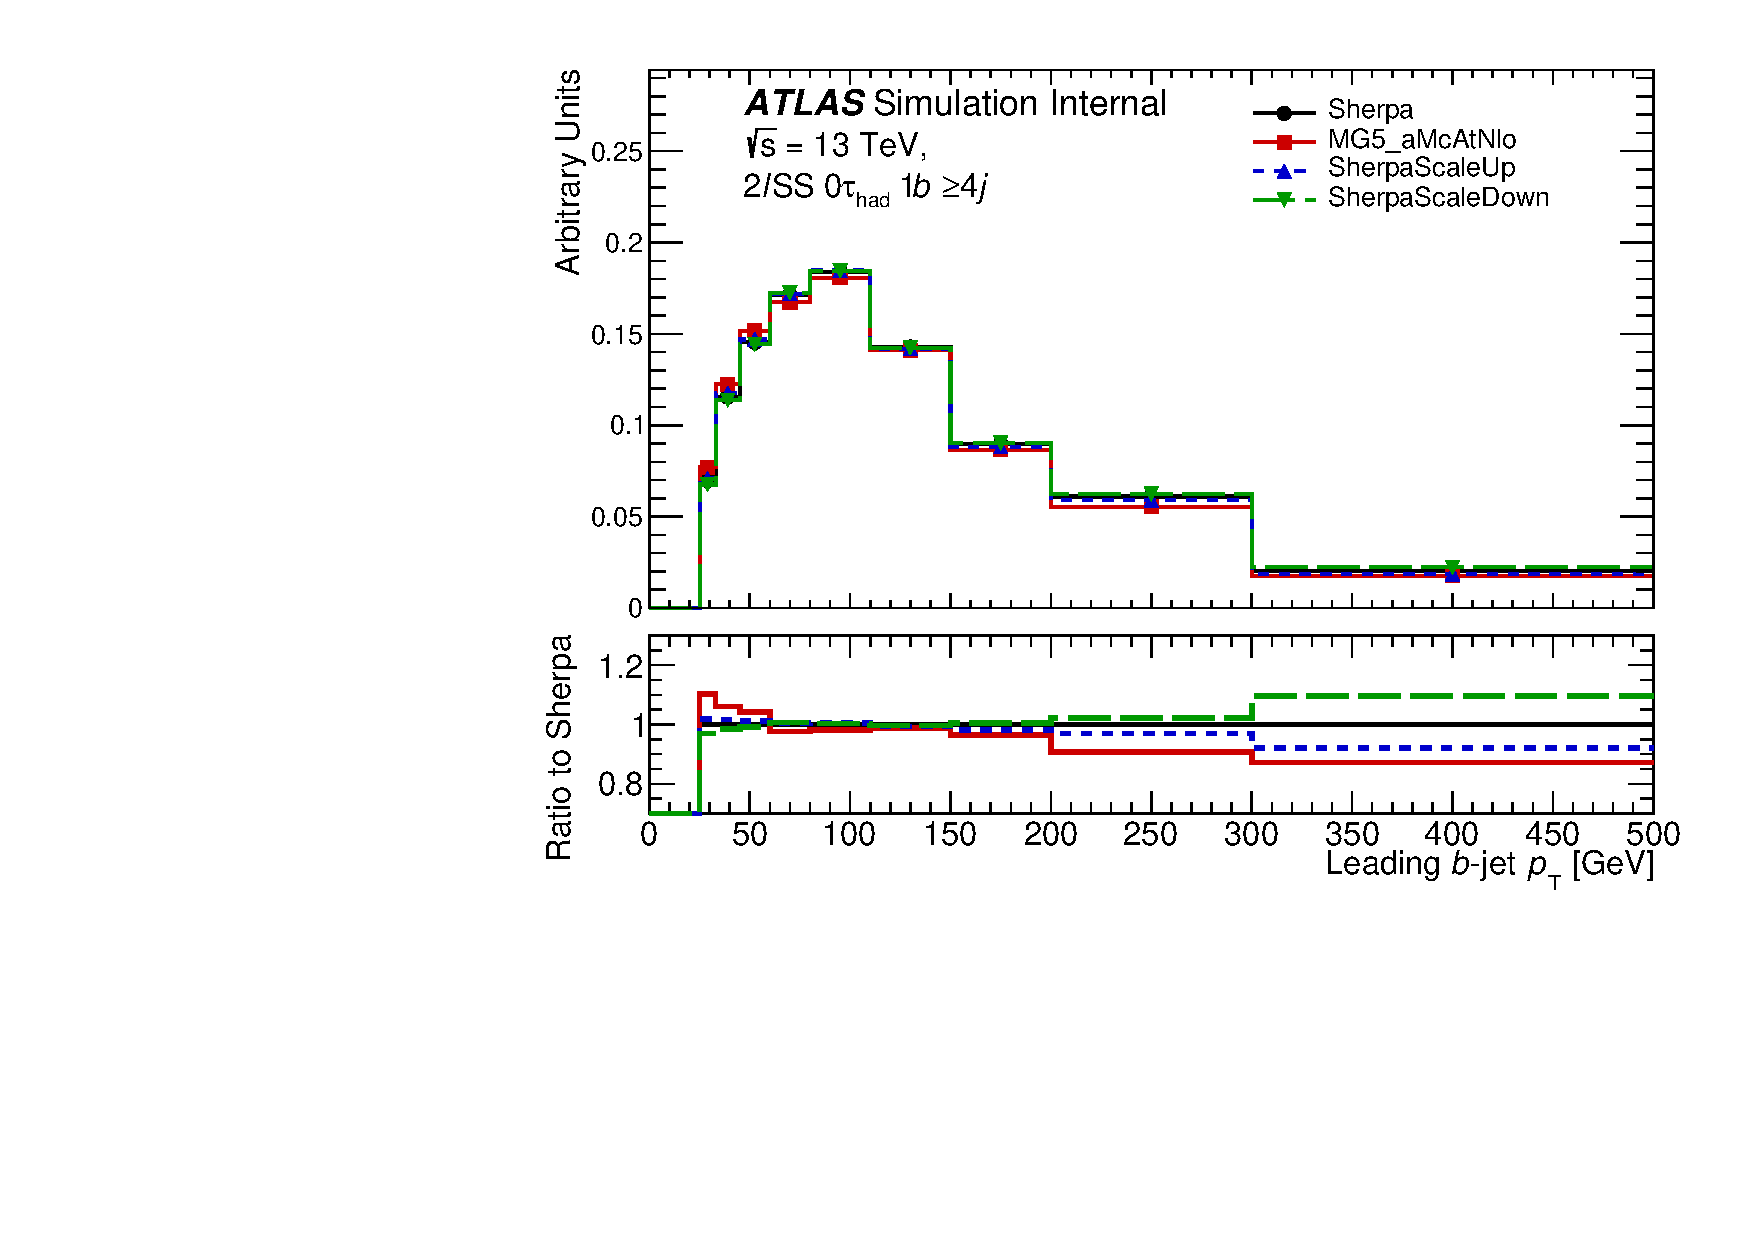
\includegraphics[width=0.45\textwidth]{Plots/ttV/shape/c_Region_0_Bjet_Pt_0}
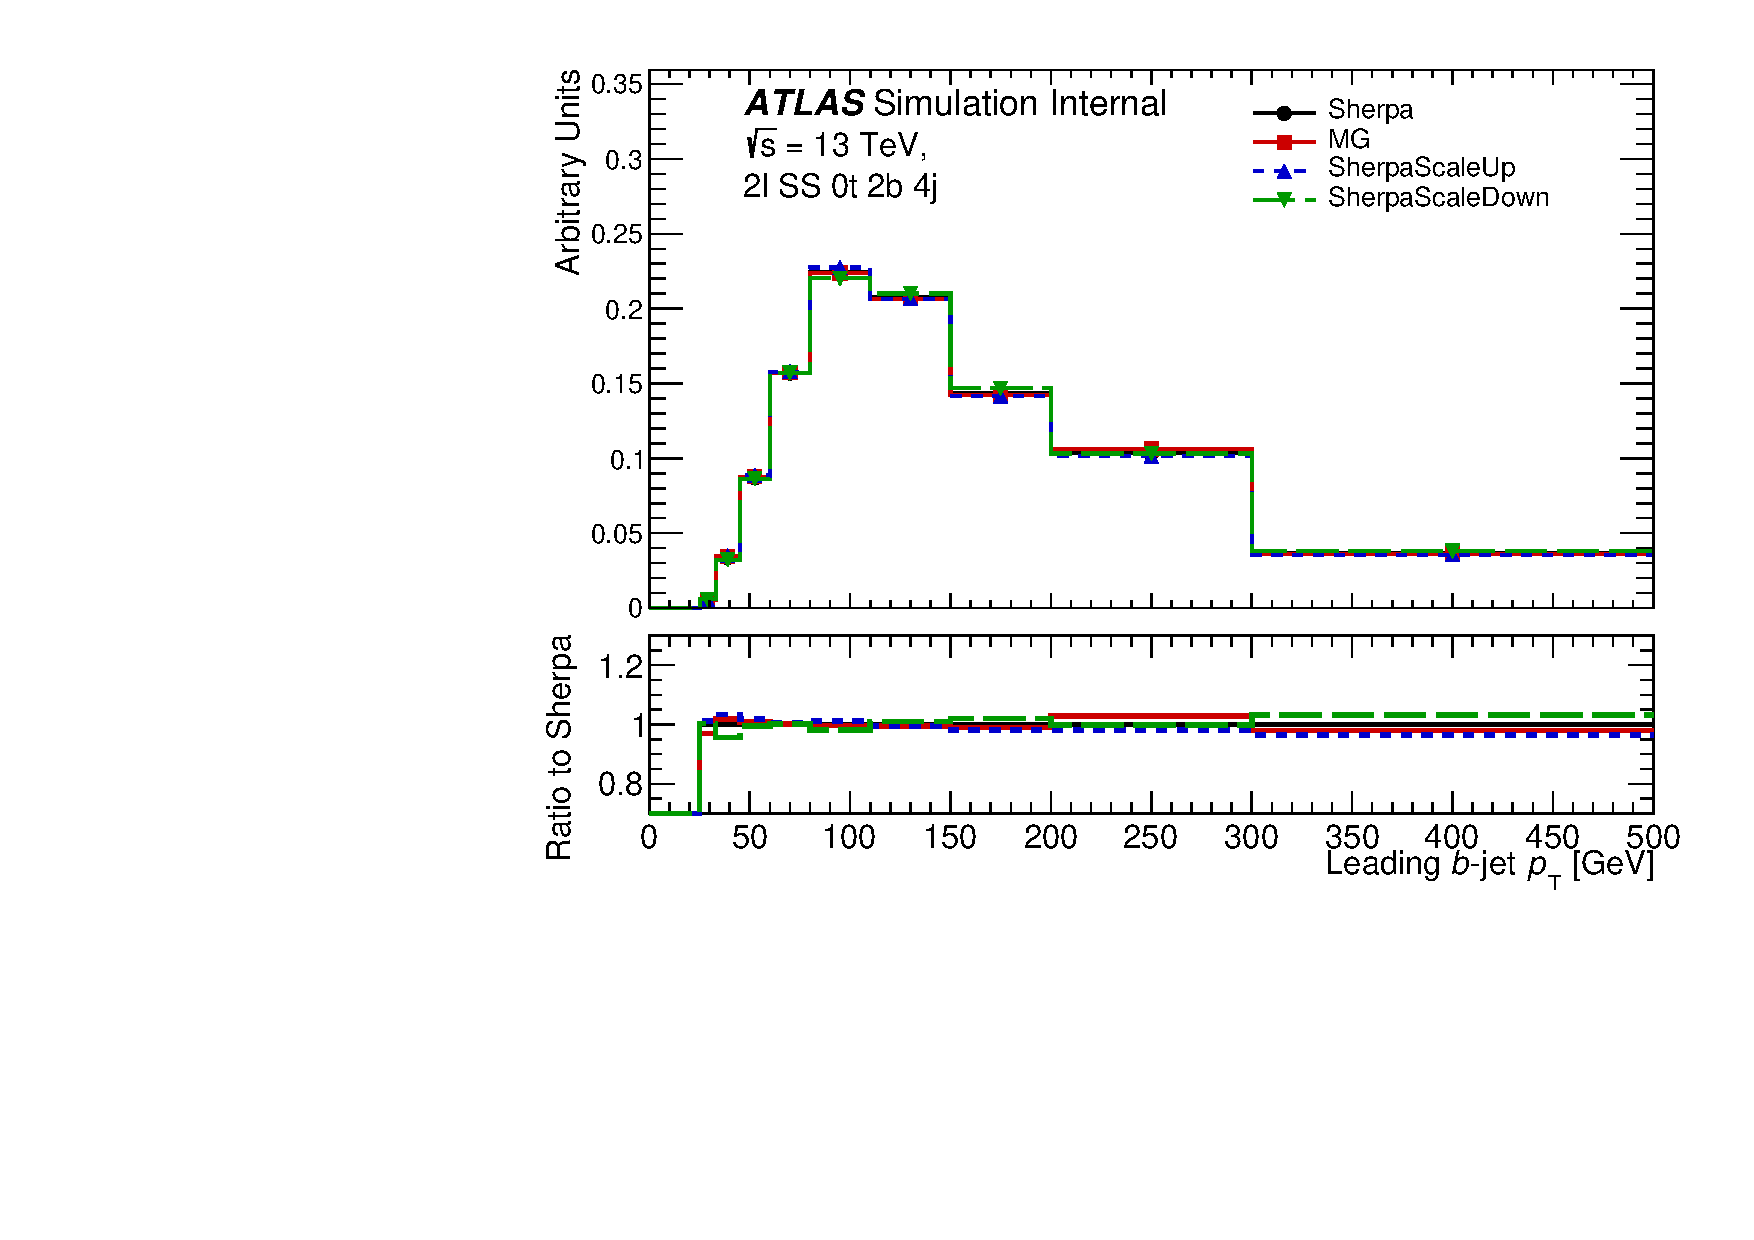
\includegraphics[width=0.45\textwidth]{Plots/ttV/shape/c_Region_1_Bjet_Pt_0}\\
  \caption{Distribution of the $b$-jet multiplicities (top) and the leading $b$-jet transverse momentum (bottom), for the Region 1 with $N_{b-\mathrm{jets}}$=1 (left) and Region 2 with $N_{b-\mathrm{jets}}\geq$2 (right) selection requiring four and more jets.  \label{ttV:4jbinfo}}
\end{figure}

Good agreement of the single lepton kinematics can be seen between nominal and alternative generators for the $N_{b-\mathrm{jets}}\geq$2 regions, as shown on the right of Figure~\ref{ttV:lep_kin} representing Region 2. Similar behaviour is also seen in Region 4.
%While there is an offset of the order of 10\%  between nominal and alternative generators for 1$b$-jet selections, as presented in the left of Figures~\ref{ttV:lep_kin} (Region 1 showed, while similar trend seen in Region 3 as well). 

Sizeable differences in shapes between nominal and alternative generators are observed for the distributions involving correlations between the two leptons.
The distributions of the angular distance between the two leptons, maximum of lepton's pseudorapidity and azimuthal separation between the leptons are presented in Figure~\ref{ttV:ll_kin} for Region 1 on the right and Region 2 on the left. 
Similar behaviour is also seen in Regions 3 and 4.
%As was observed for single lepton kinematics, difference in 1$b$-jet selections is increased wrt to $\geq2b$-jets selection.
%Distributions are presented for $\geq2N_{b-jets},\geq4N_{jets}$ region, while similar behaviour seen in all other regions as well.

Distributions of the jet multiplicity, number of $b$-jets, the leading lepton transverse momentum and the angular distance between the two leptons  $\Delta R _{\ell 0\ell1 }$ for the Region 5 with $N_{\tau_\mathrm{had}}$ = 1 selection are presented in Figure ~\ref{ttV:tauR_kin}.
The difference observed between nominal and alternative generators for high jet multiplicities, at the edge of the scale variation uncertainty band. 
The distribution of $N_{b-\mathrm{jets}}$ is in agreement for $N_{b-\mathrm{jets}}$ = 2, while a sizeable difference is observed for $N_{b-\mathrm{jets}} = 1$, which is similar to the $N_{\tau_\mathrm{had}}$ = 0 selections. 
Lepton kinematic distributions show differences in shapes between the nominal and alternative generator.

\begin{figure}[!htb]
\centering
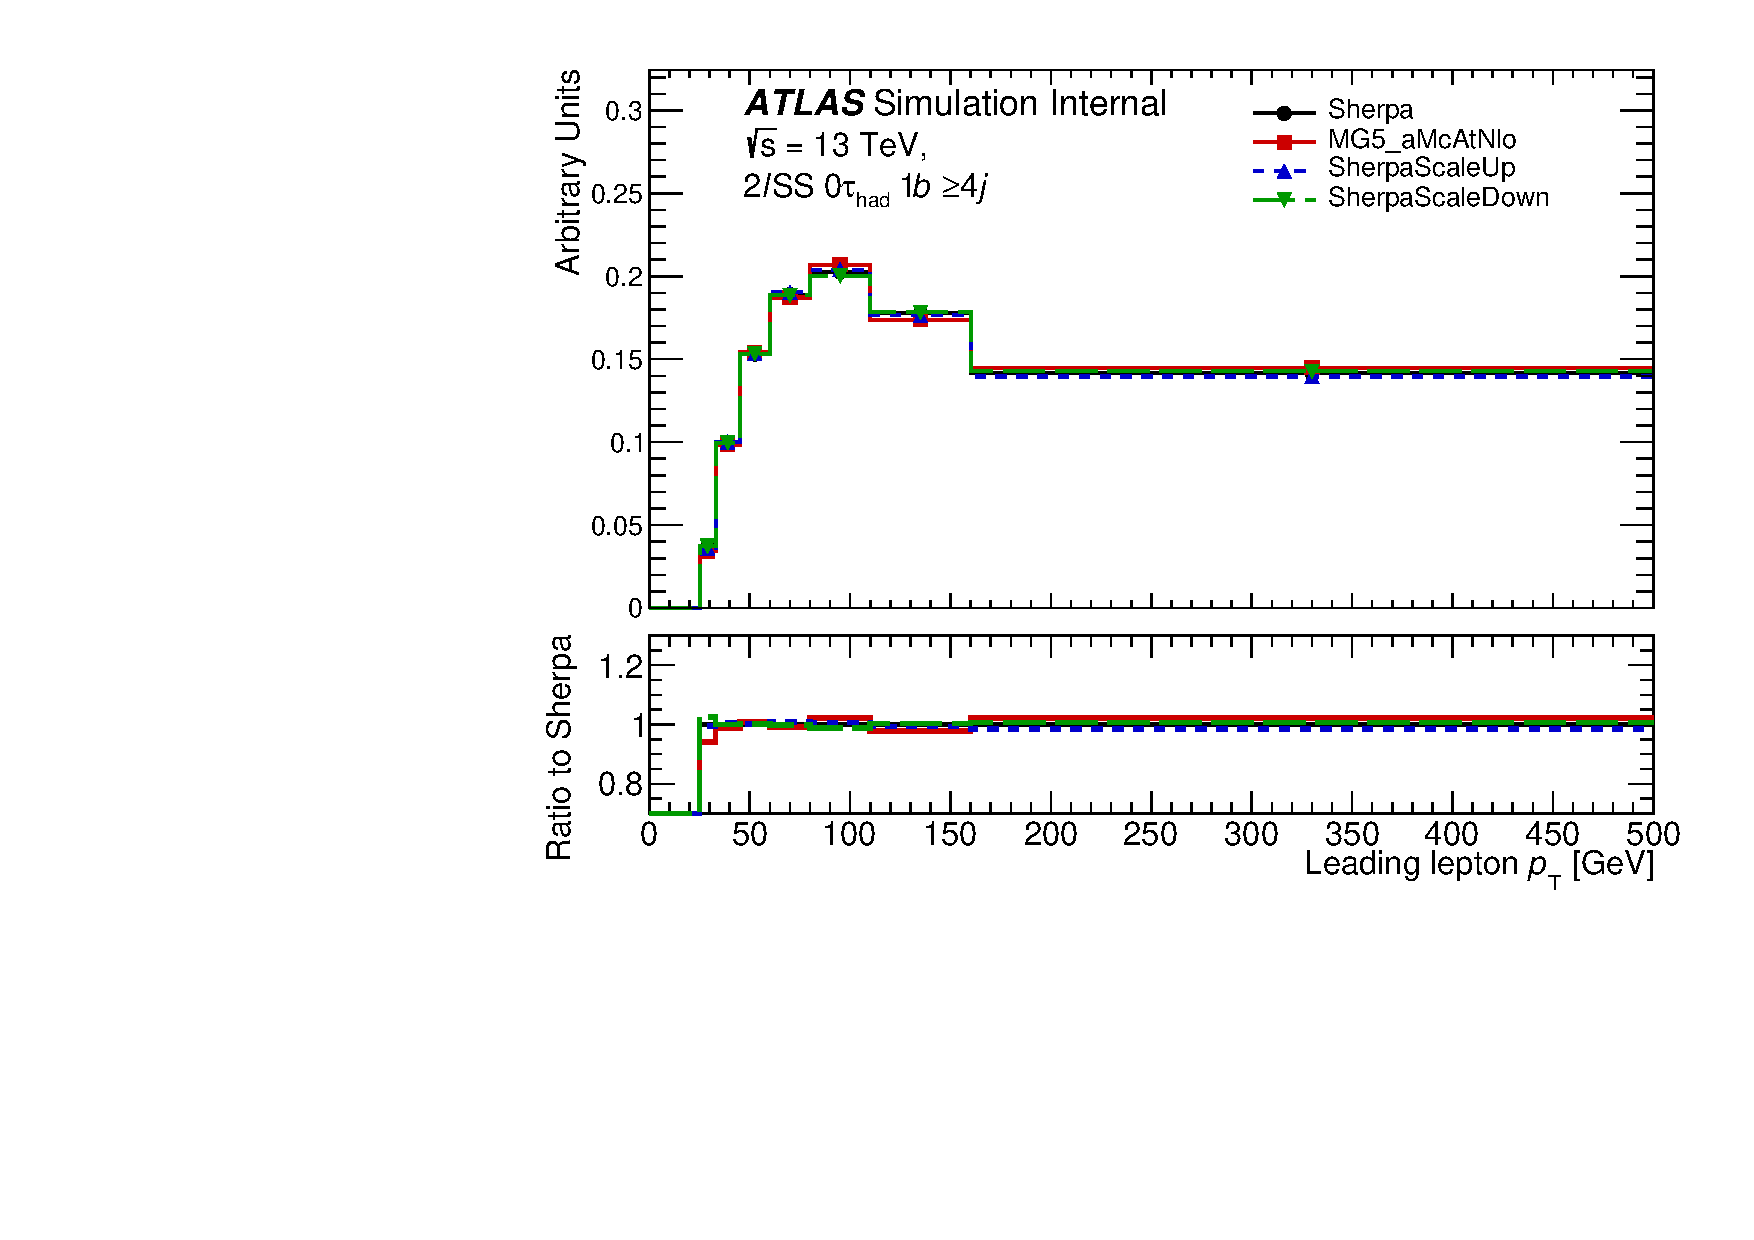
\includegraphics[width=0.45\textwidth]{Plots/ttV/shape/c_Region_0_lep_Pt_0}
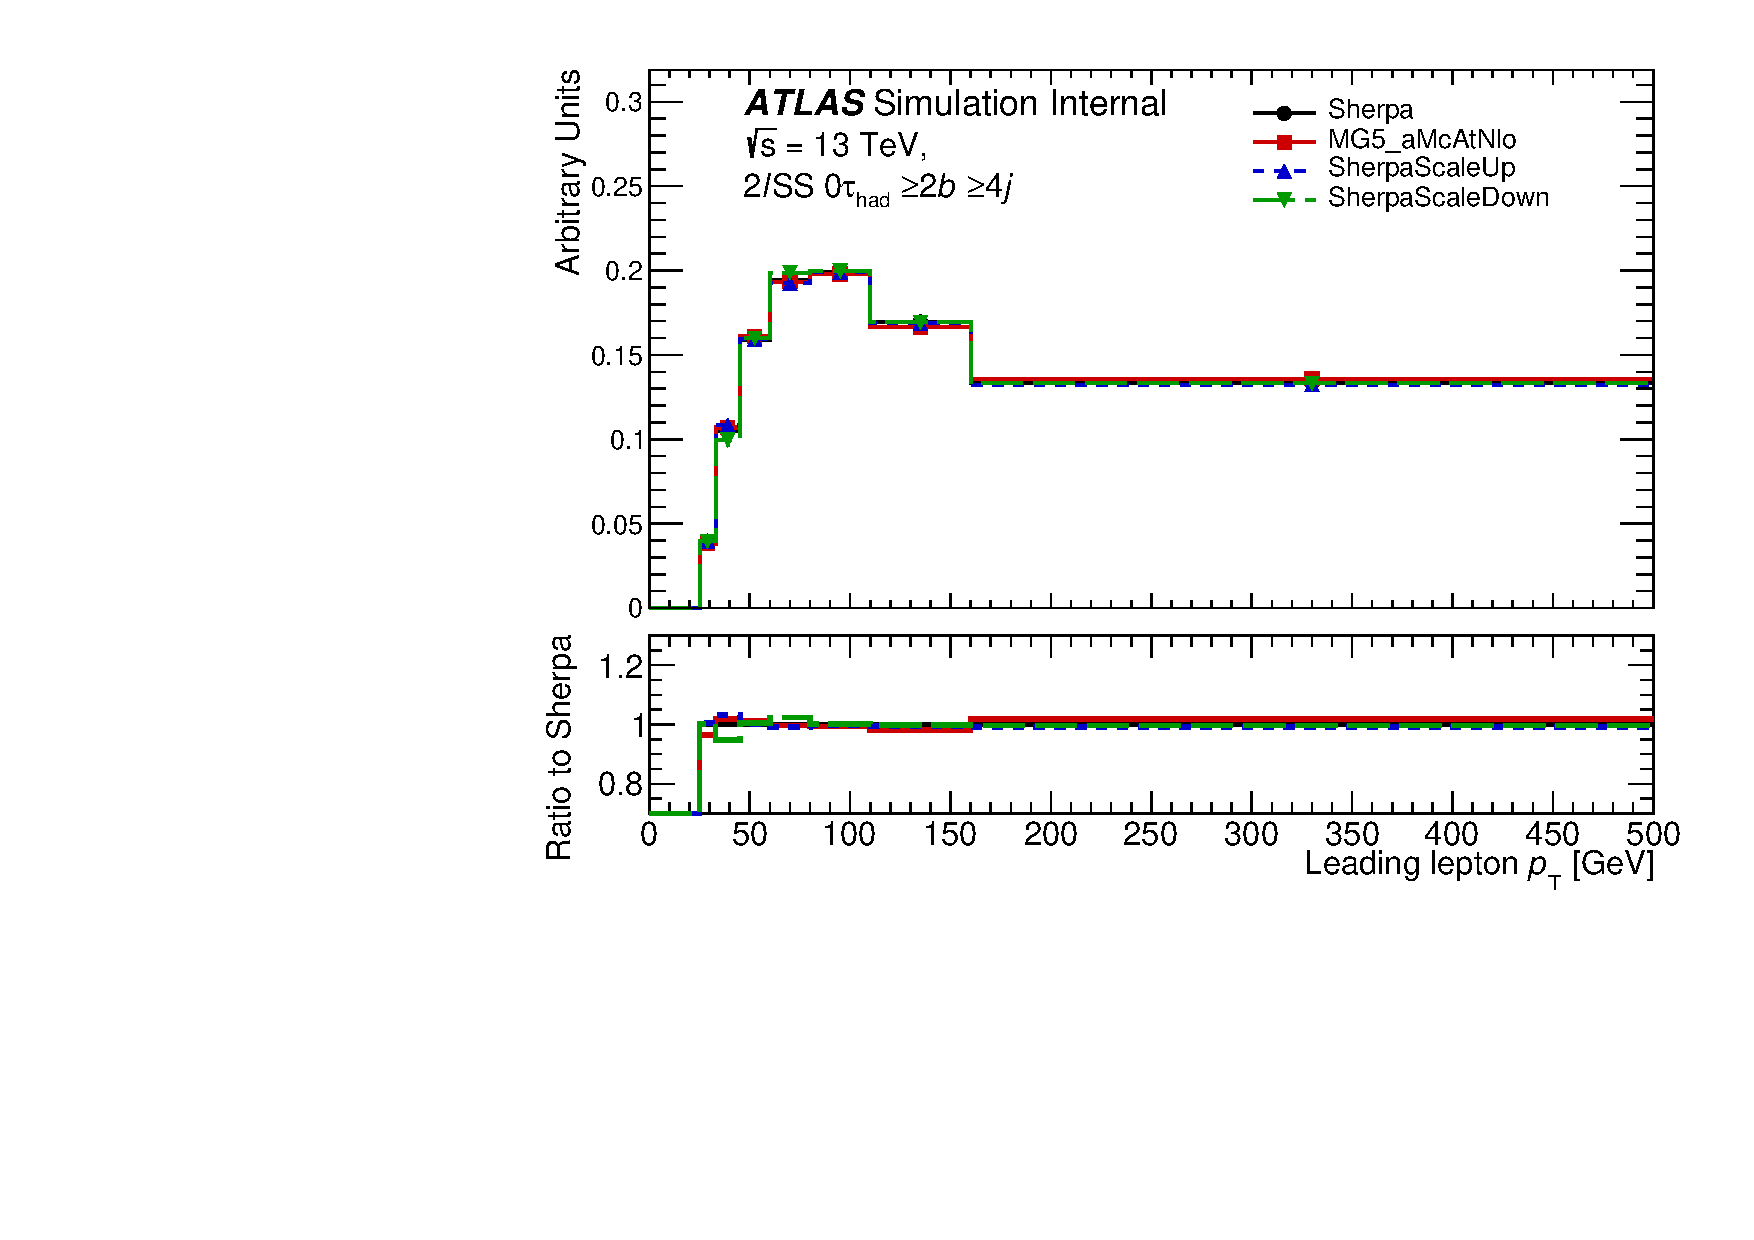
\includegraphics[width=0.45\textwidth]{Plots/ttV/shape/c_Region_1_lep_Pt_0}\\
%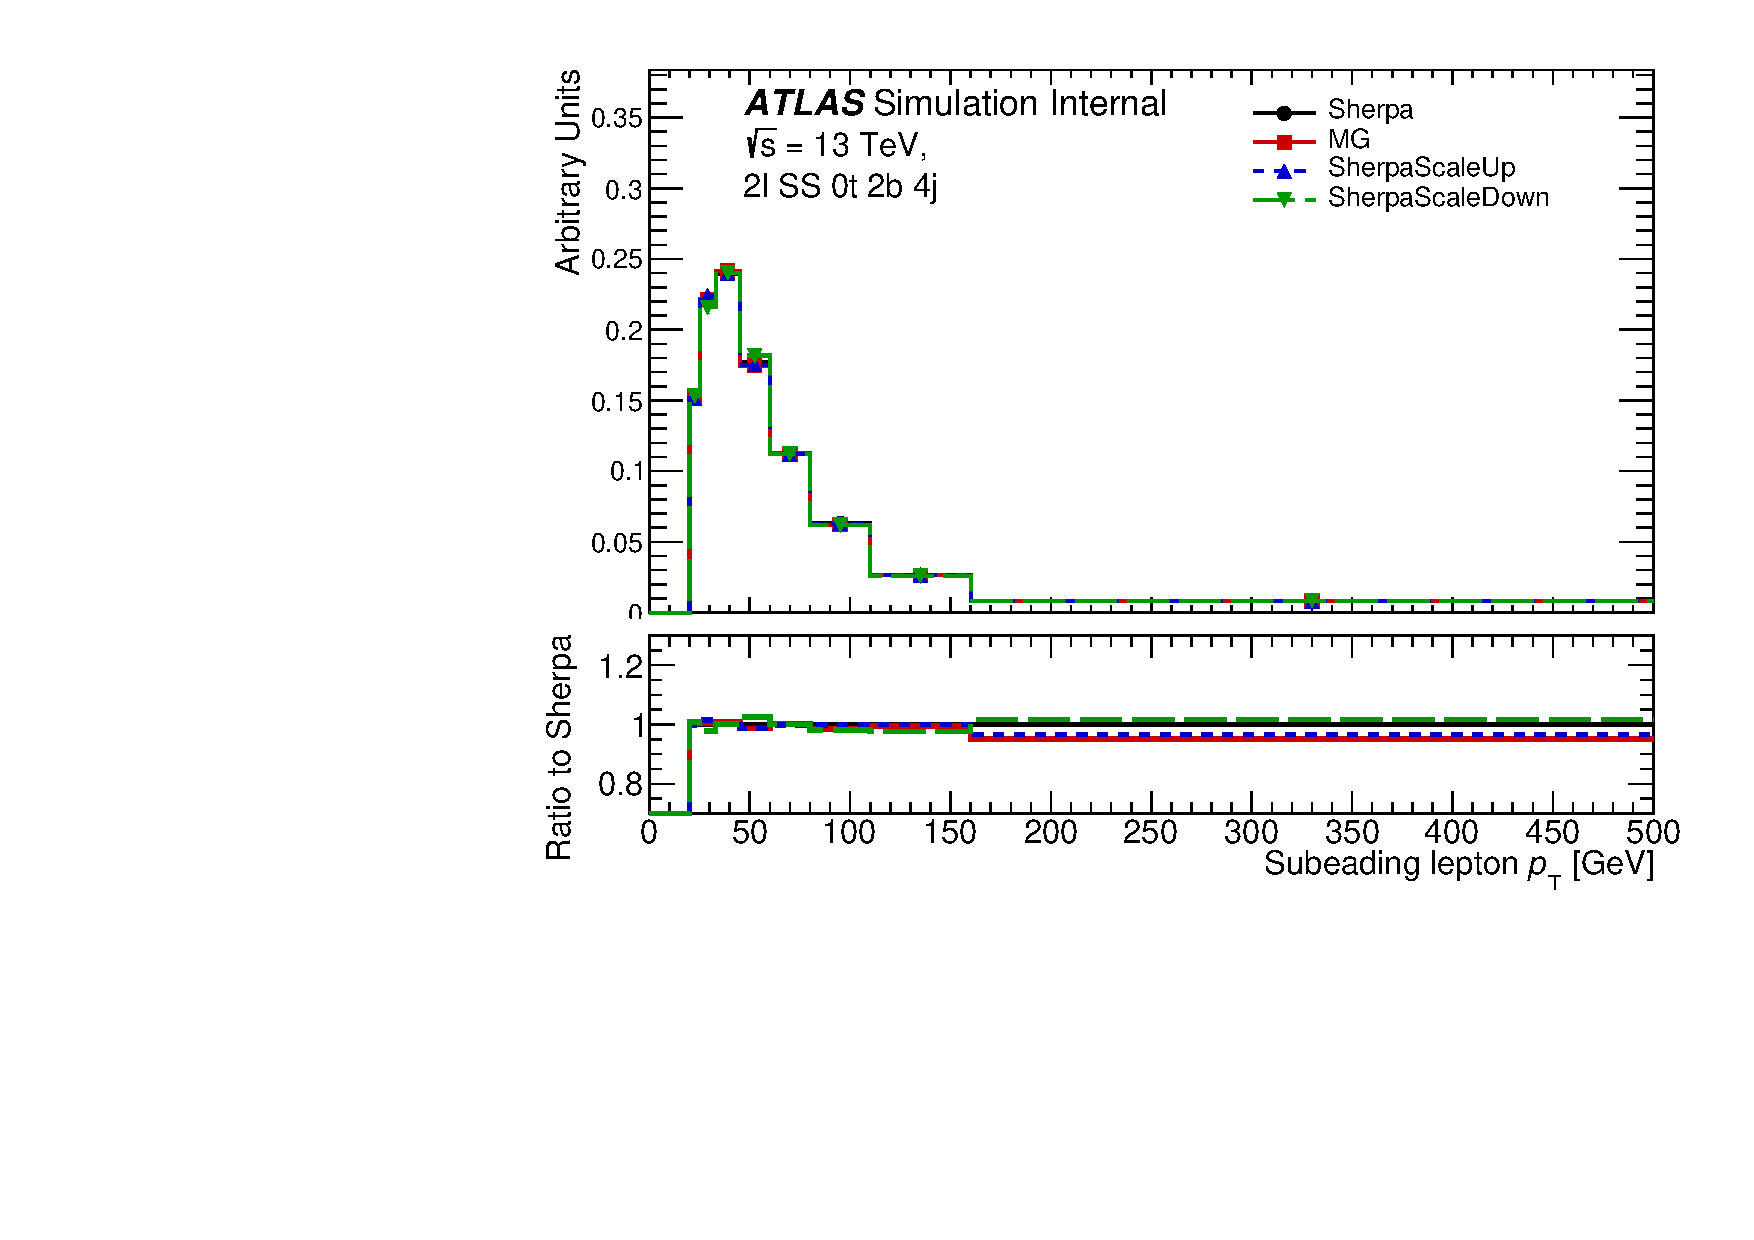
\includegraphics[width=0.45\textwidth]{Plots/ttV/shape/c_Region_1_lep_Pt_1}
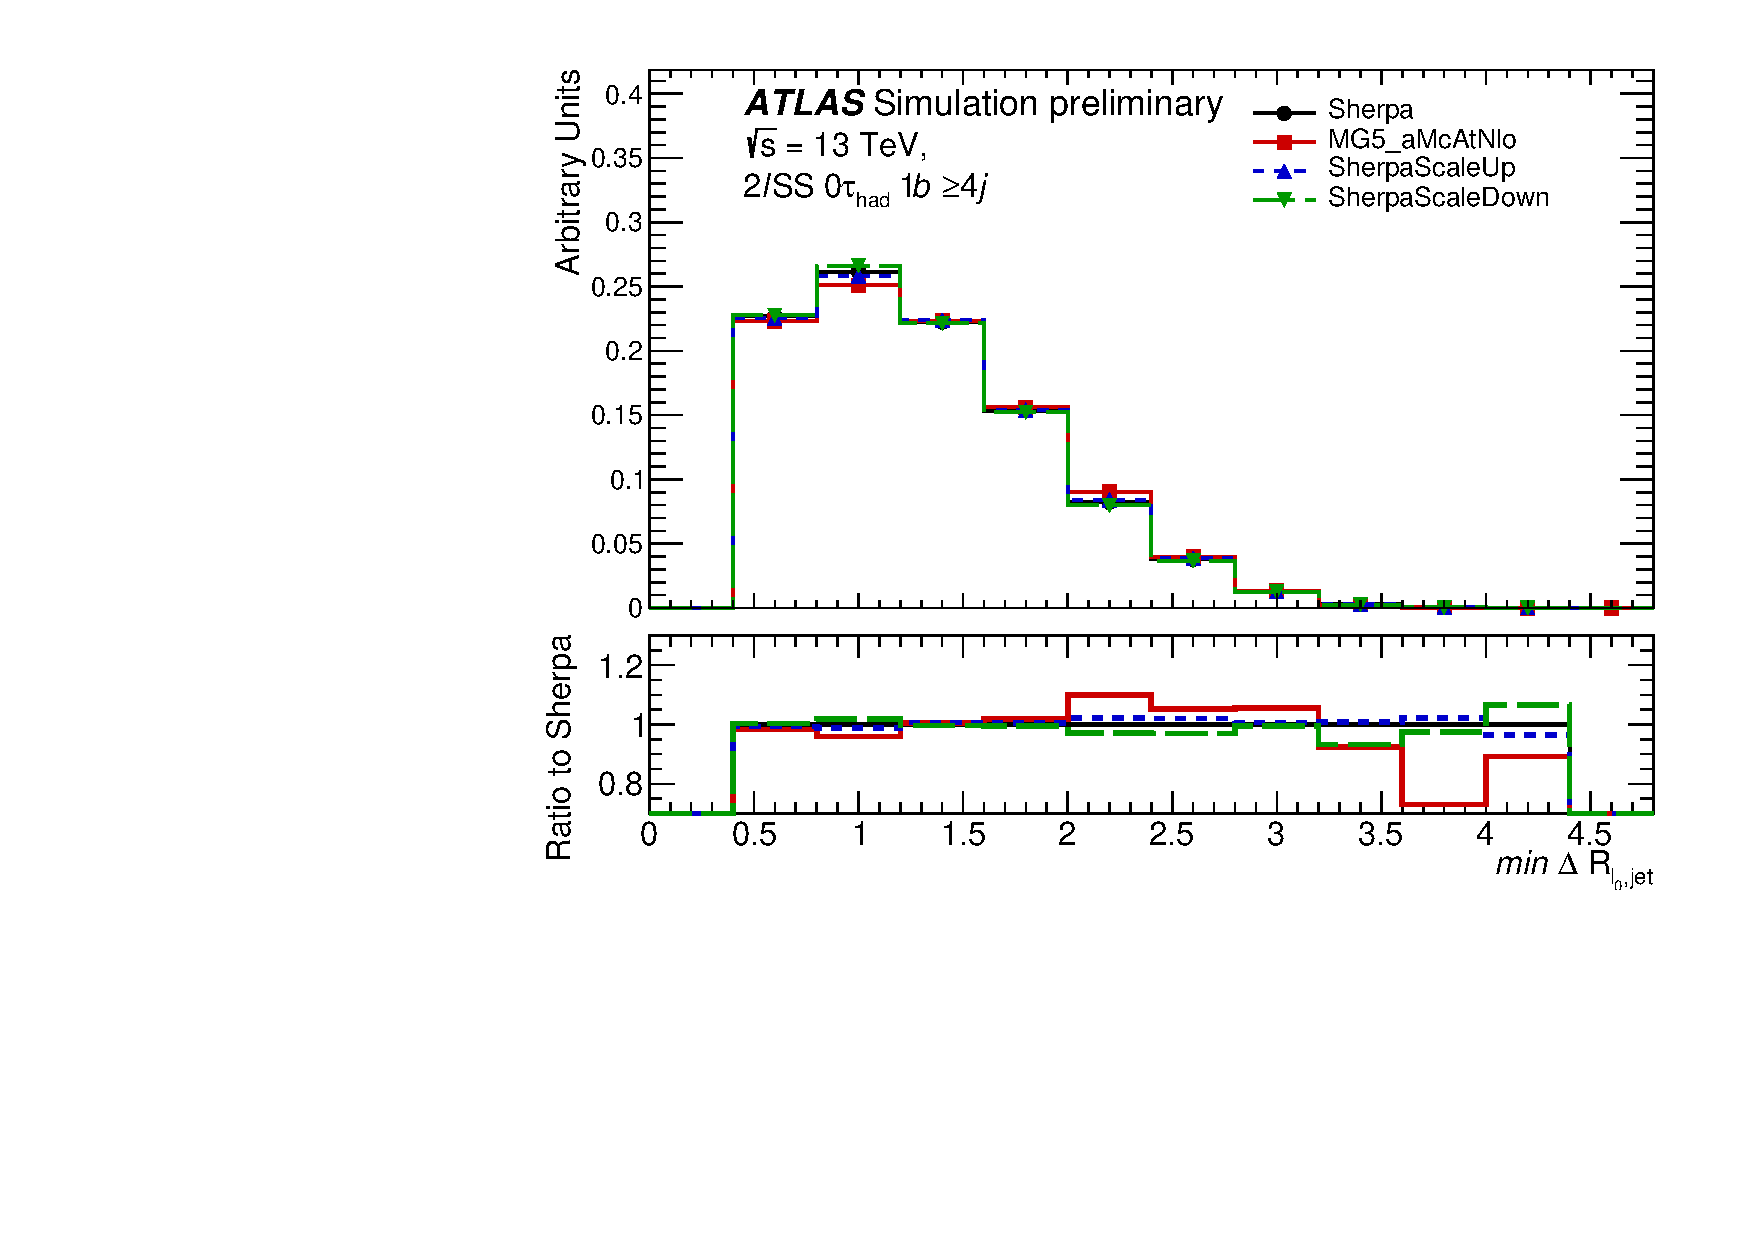
\includegraphics[width=0.45\textwidth]{Plots/ttV/shape/c_Region_0_min_DRl0j}
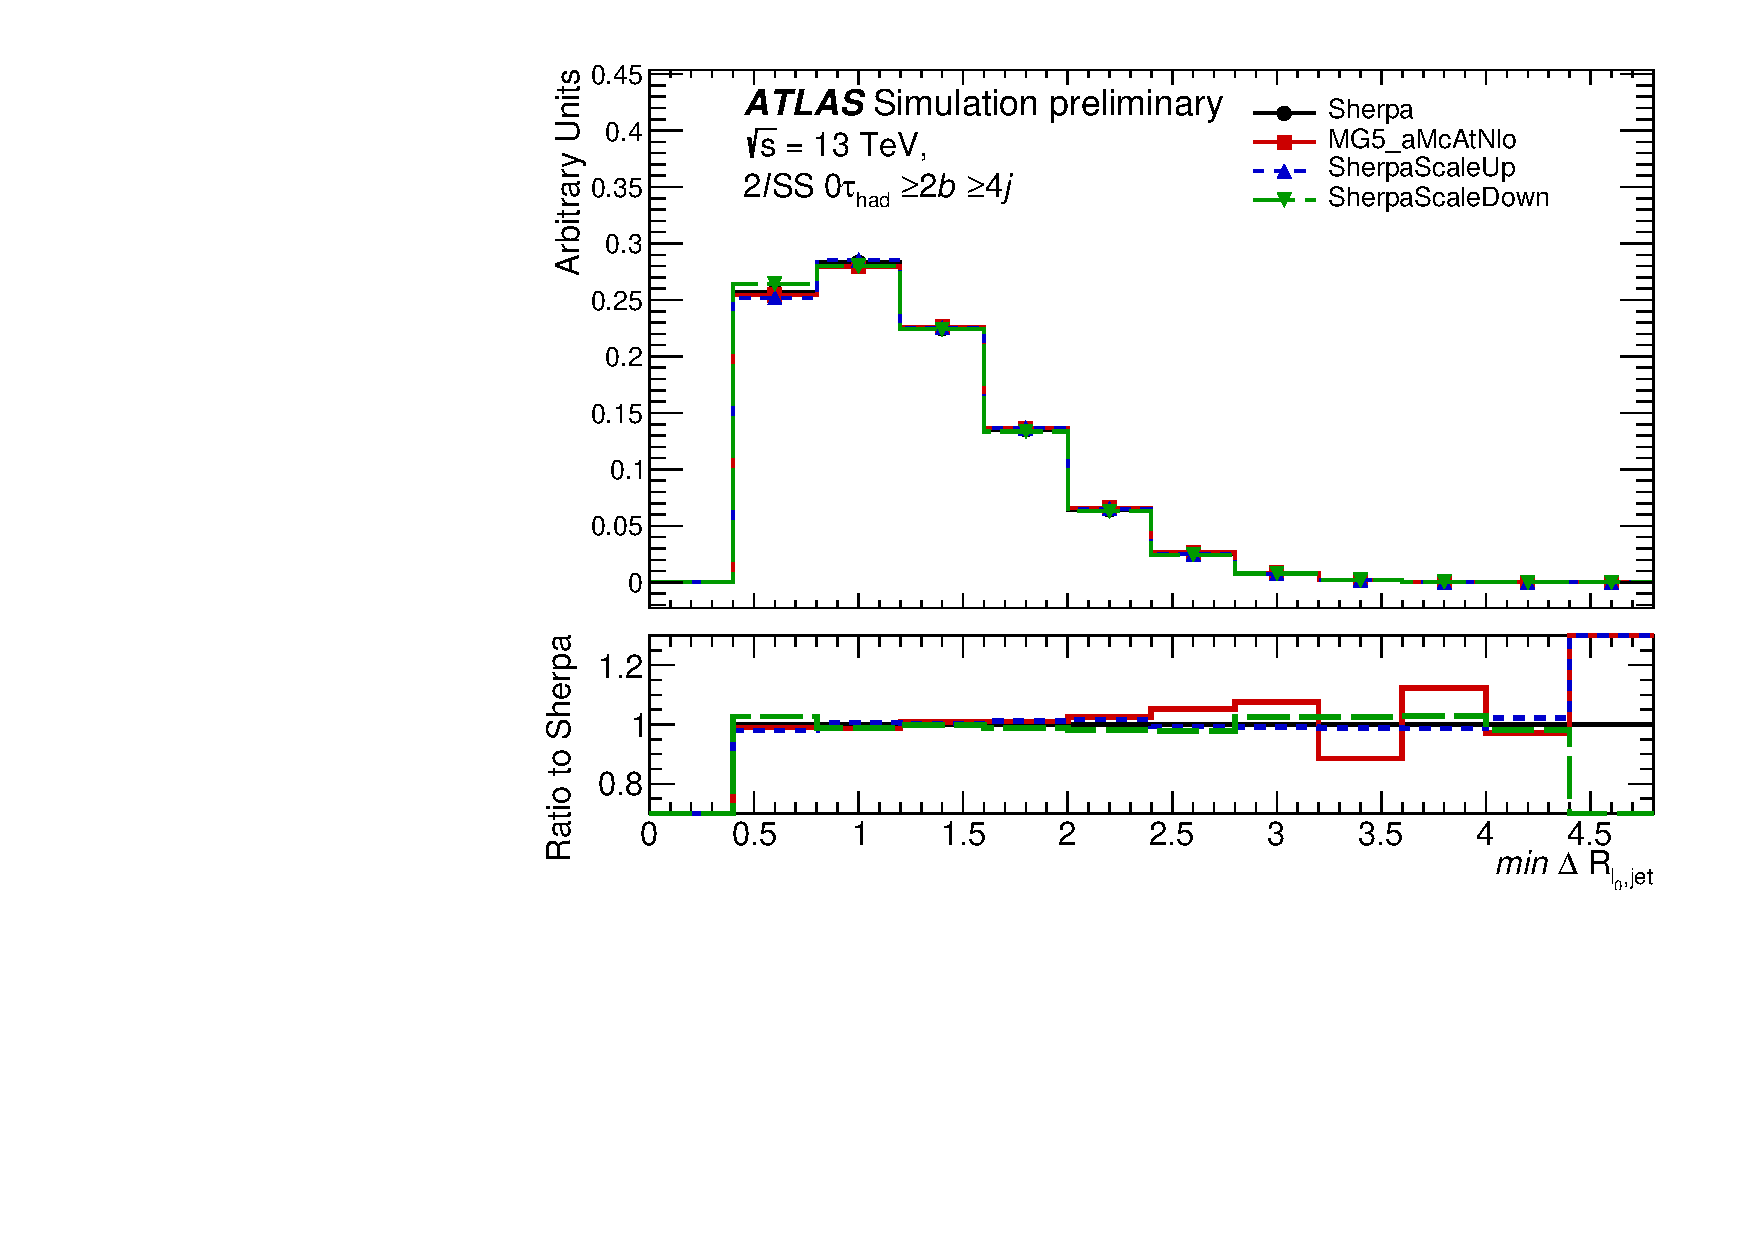
\includegraphics[width=0.45\textwidth]{Plots/ttV/shape/c_Region_1_min_DRl0j}\\
  \caption{Distribution of the leading lepton transverse momentum (top) and the minimum angular separation between the leading lepton and the nearest jet (bottom), for the Region 1 with $N_{b-\mathrm{jets}}$=1(left) and Region 2 with $N_{b-\mathrm{jets}}\geq$2(right) selection requiring four and more jets. 
  \label{ttV:lep_kin}}
\end{figure}

\begin{figure}[!htb]
\centering
	% \hspace{25mm} $DRl_0l_1$  \hspace{20mm} $max|\eta^{\ell\ell}|$\\
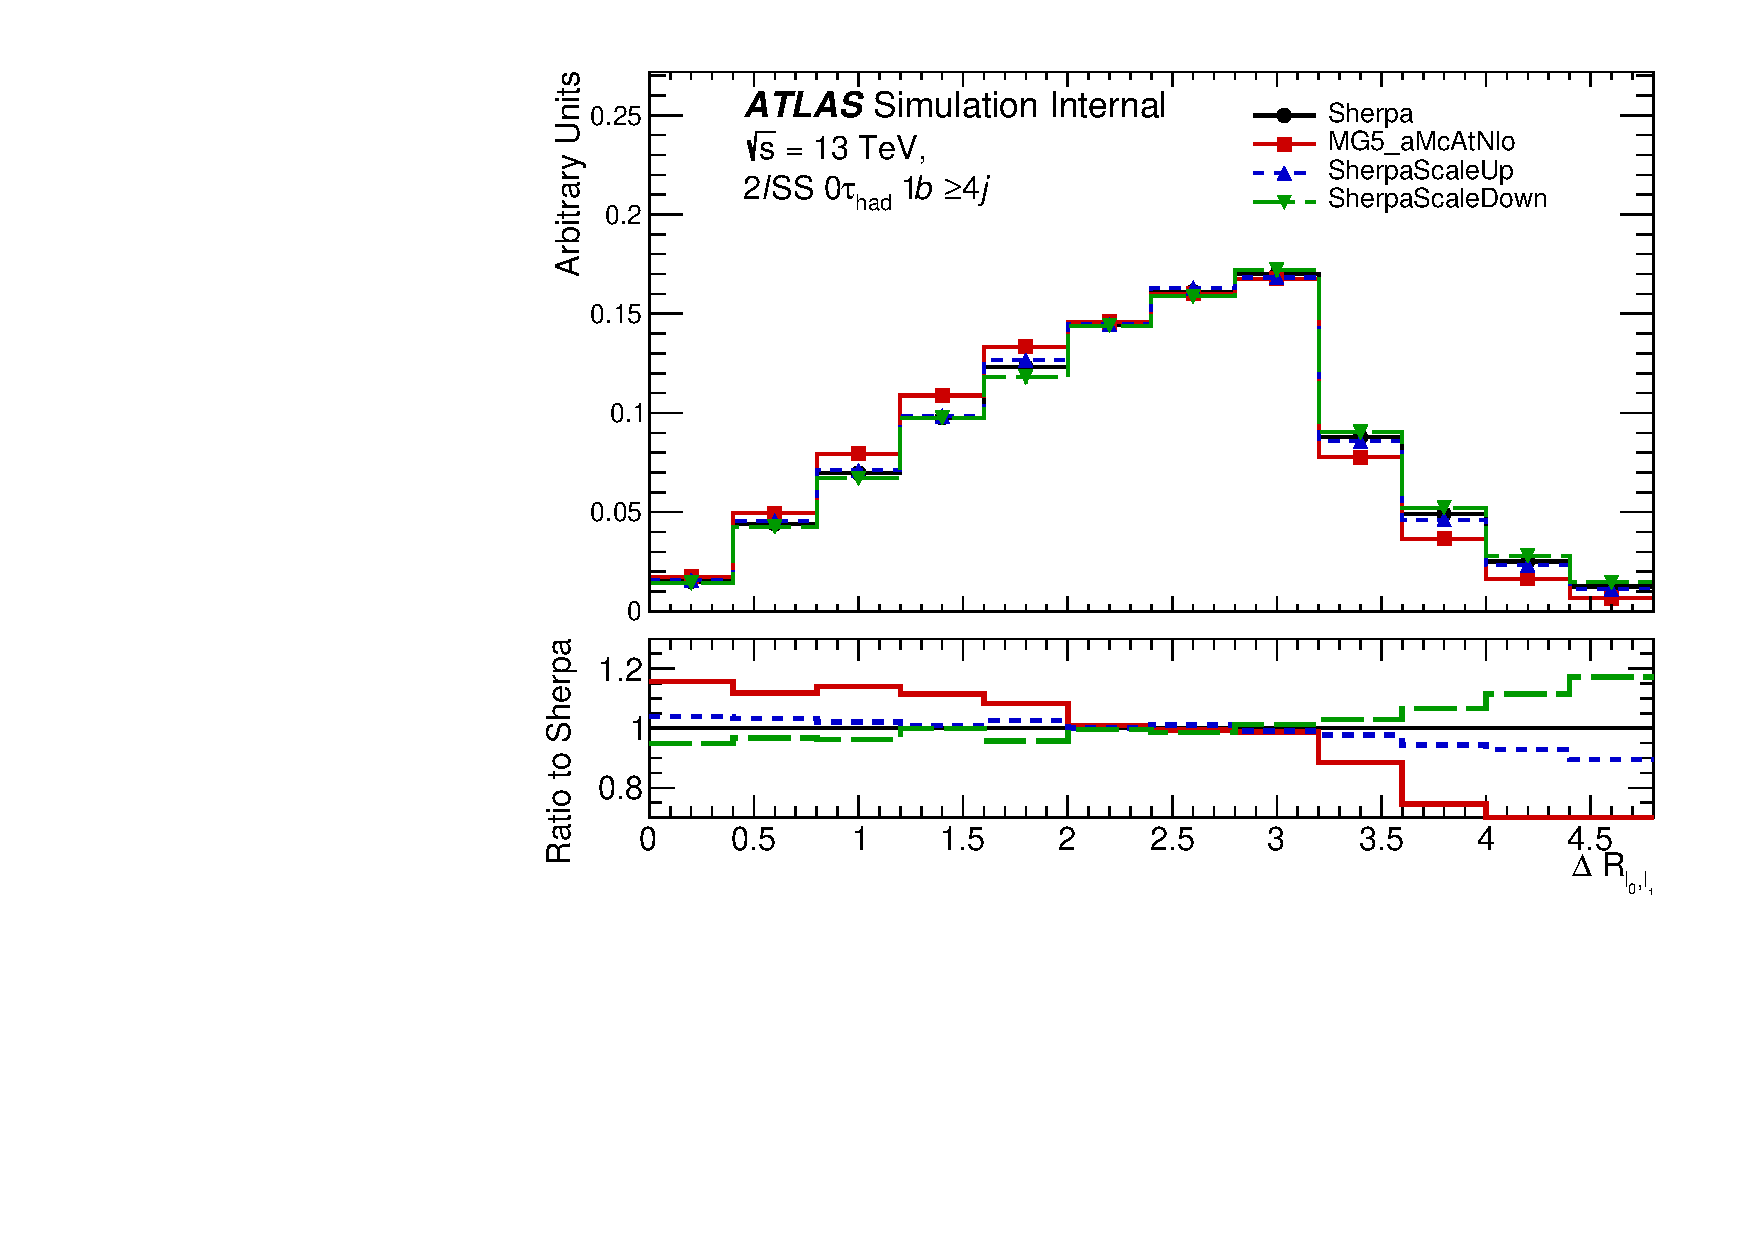
\includegraphics[width=0.45\textwidth]{Plots/ttV/shape/c_Region_0_DRll01}
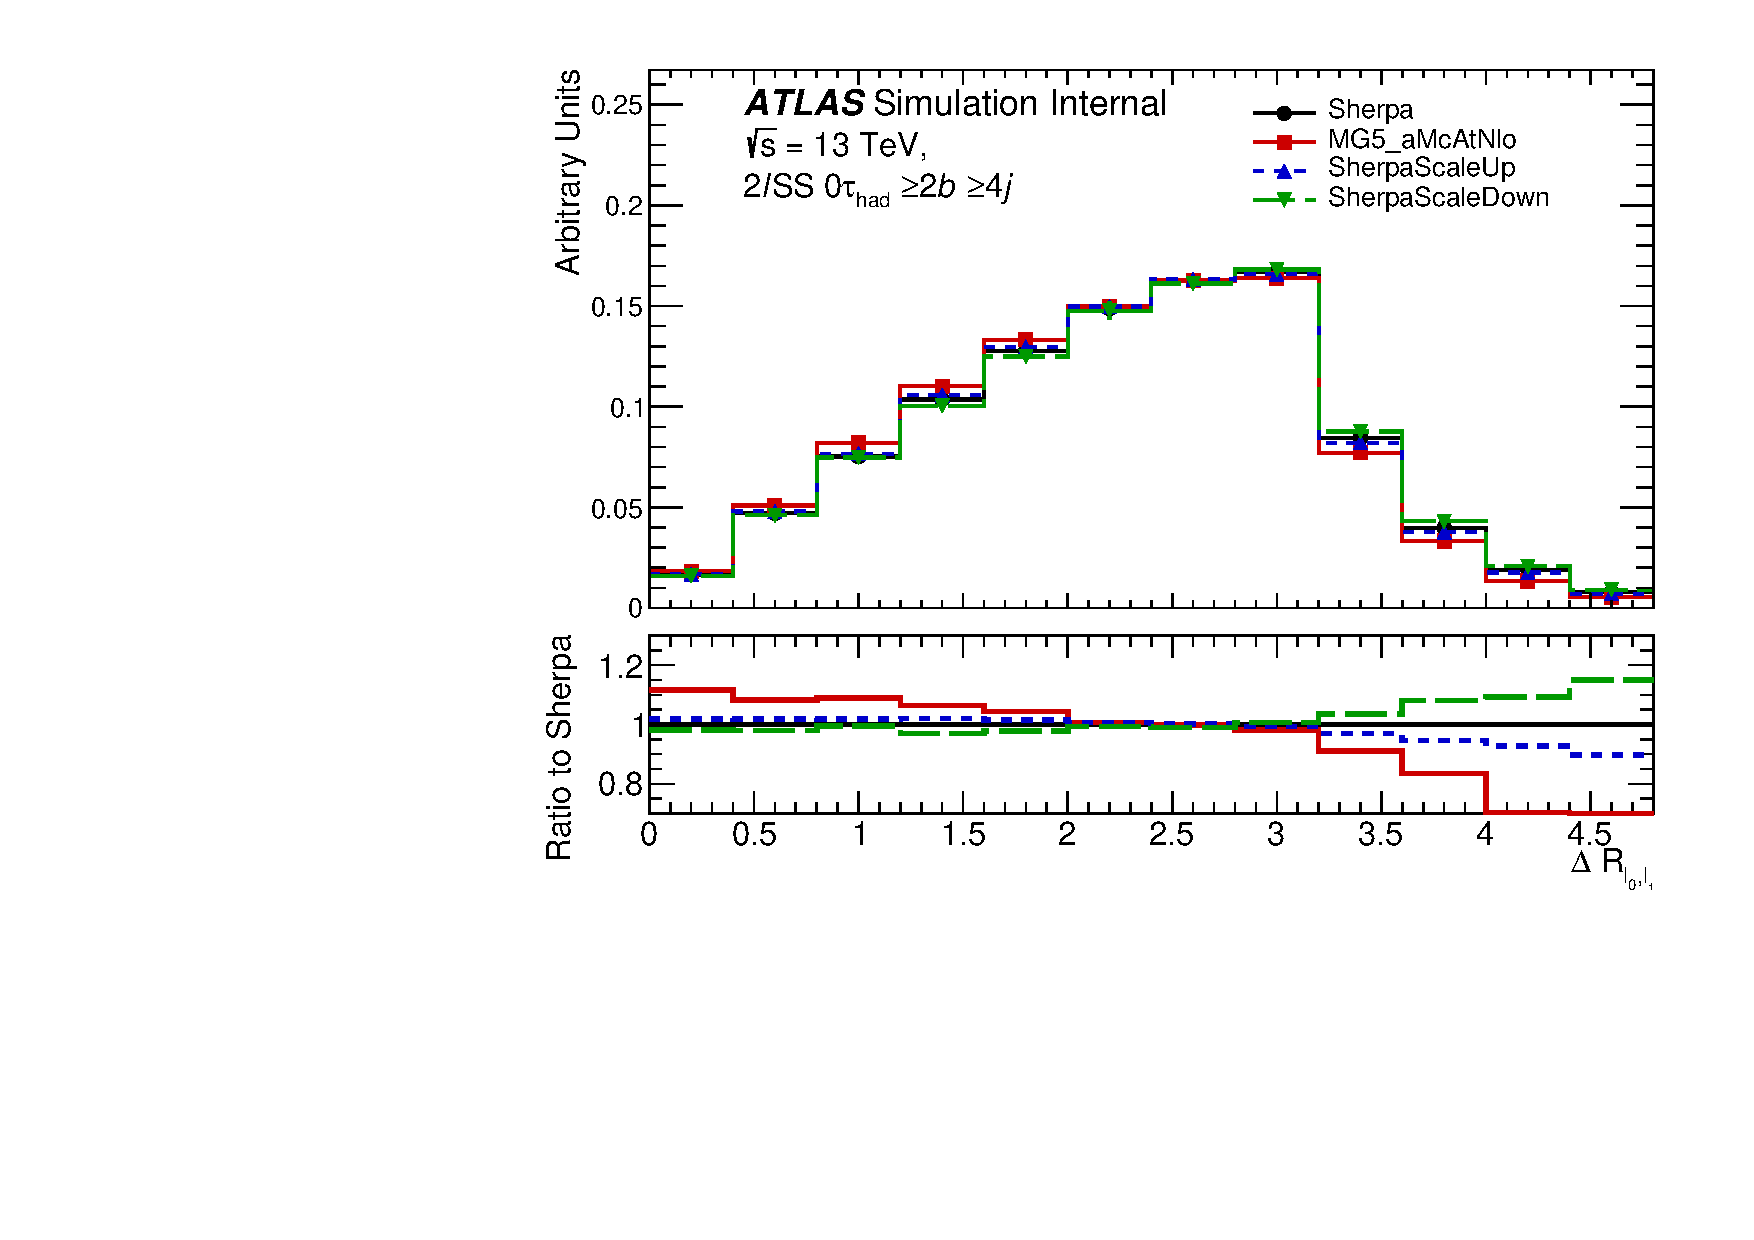
\includegraphics[width=0.45\textwidth]{Plots/ttV/shape/c_Region_1_DRll01}\\
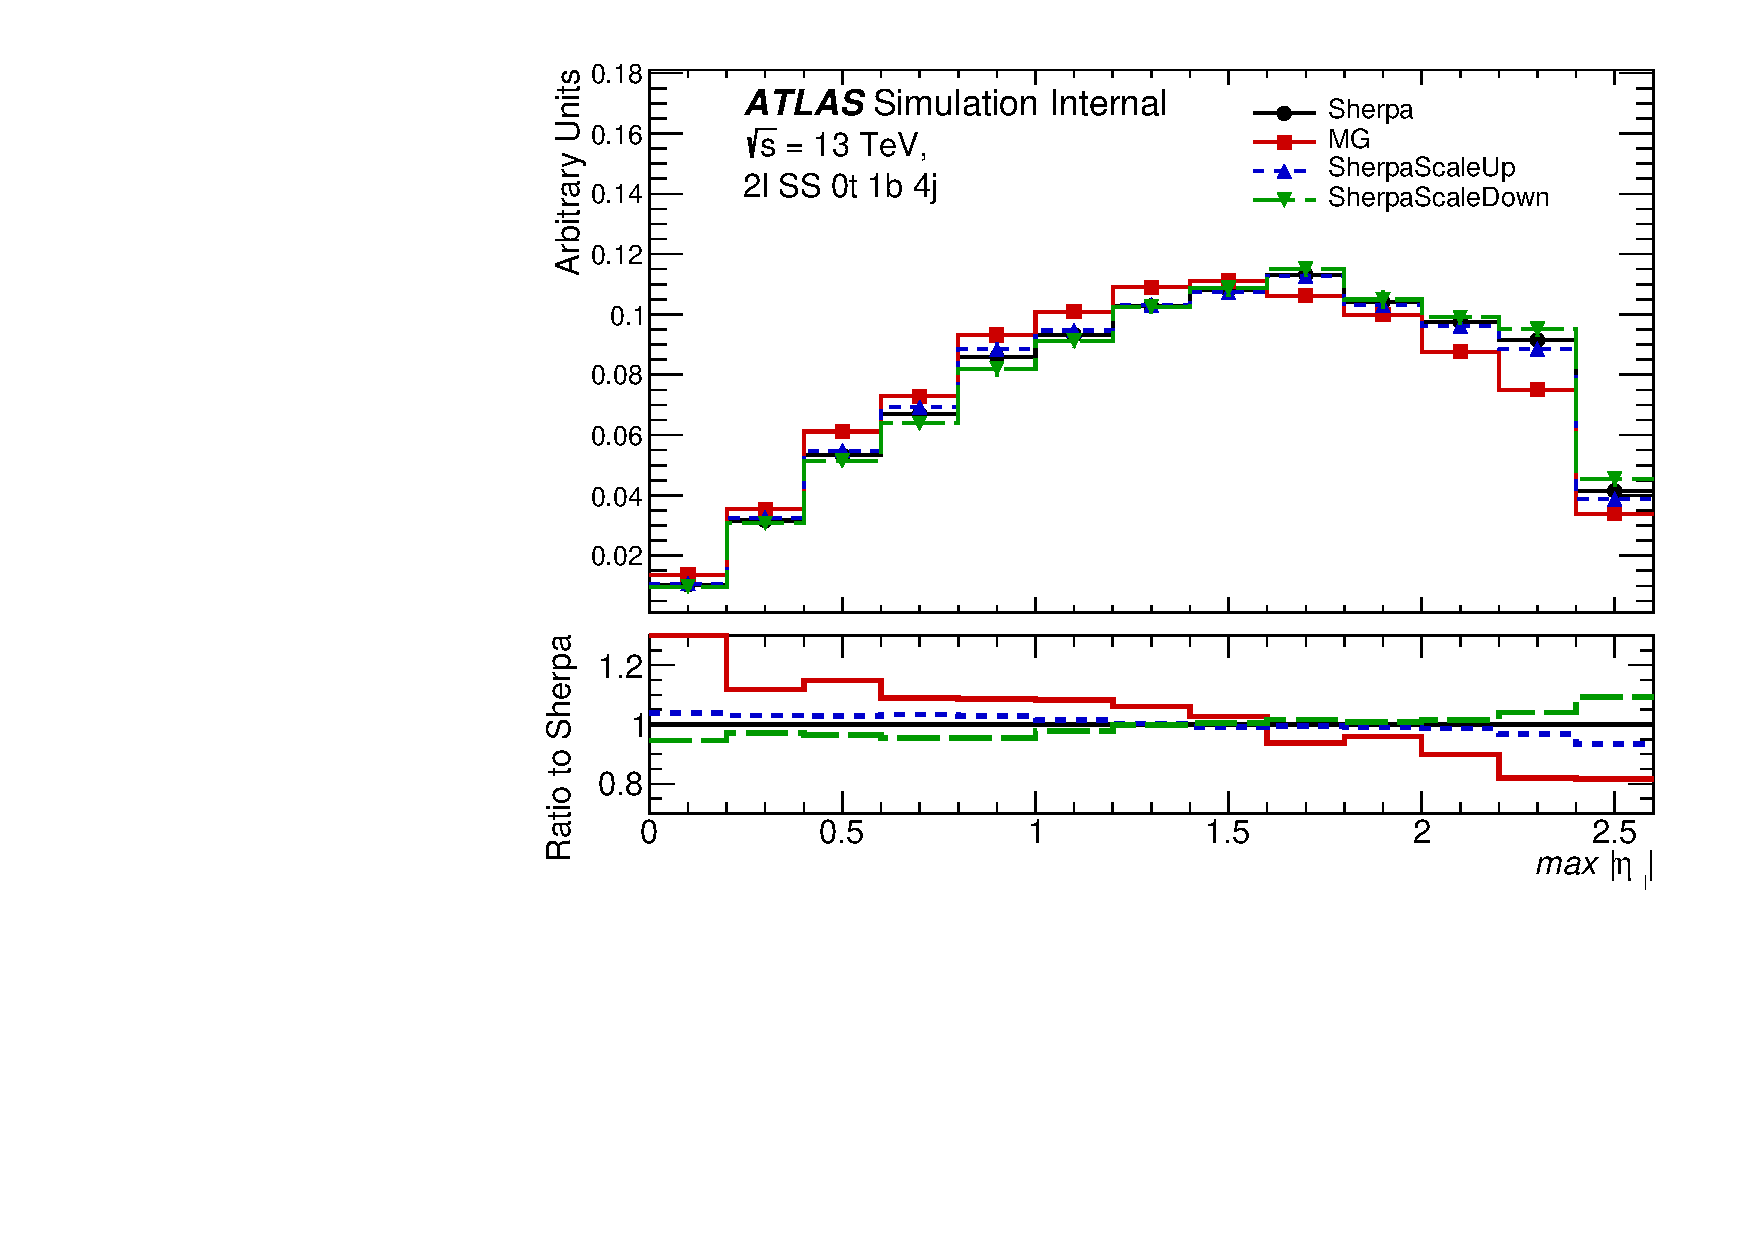
\includegraphics[width=0.45\textwidth]{Plots/ttV/shape/c_Region_0_maxEta_ll} 
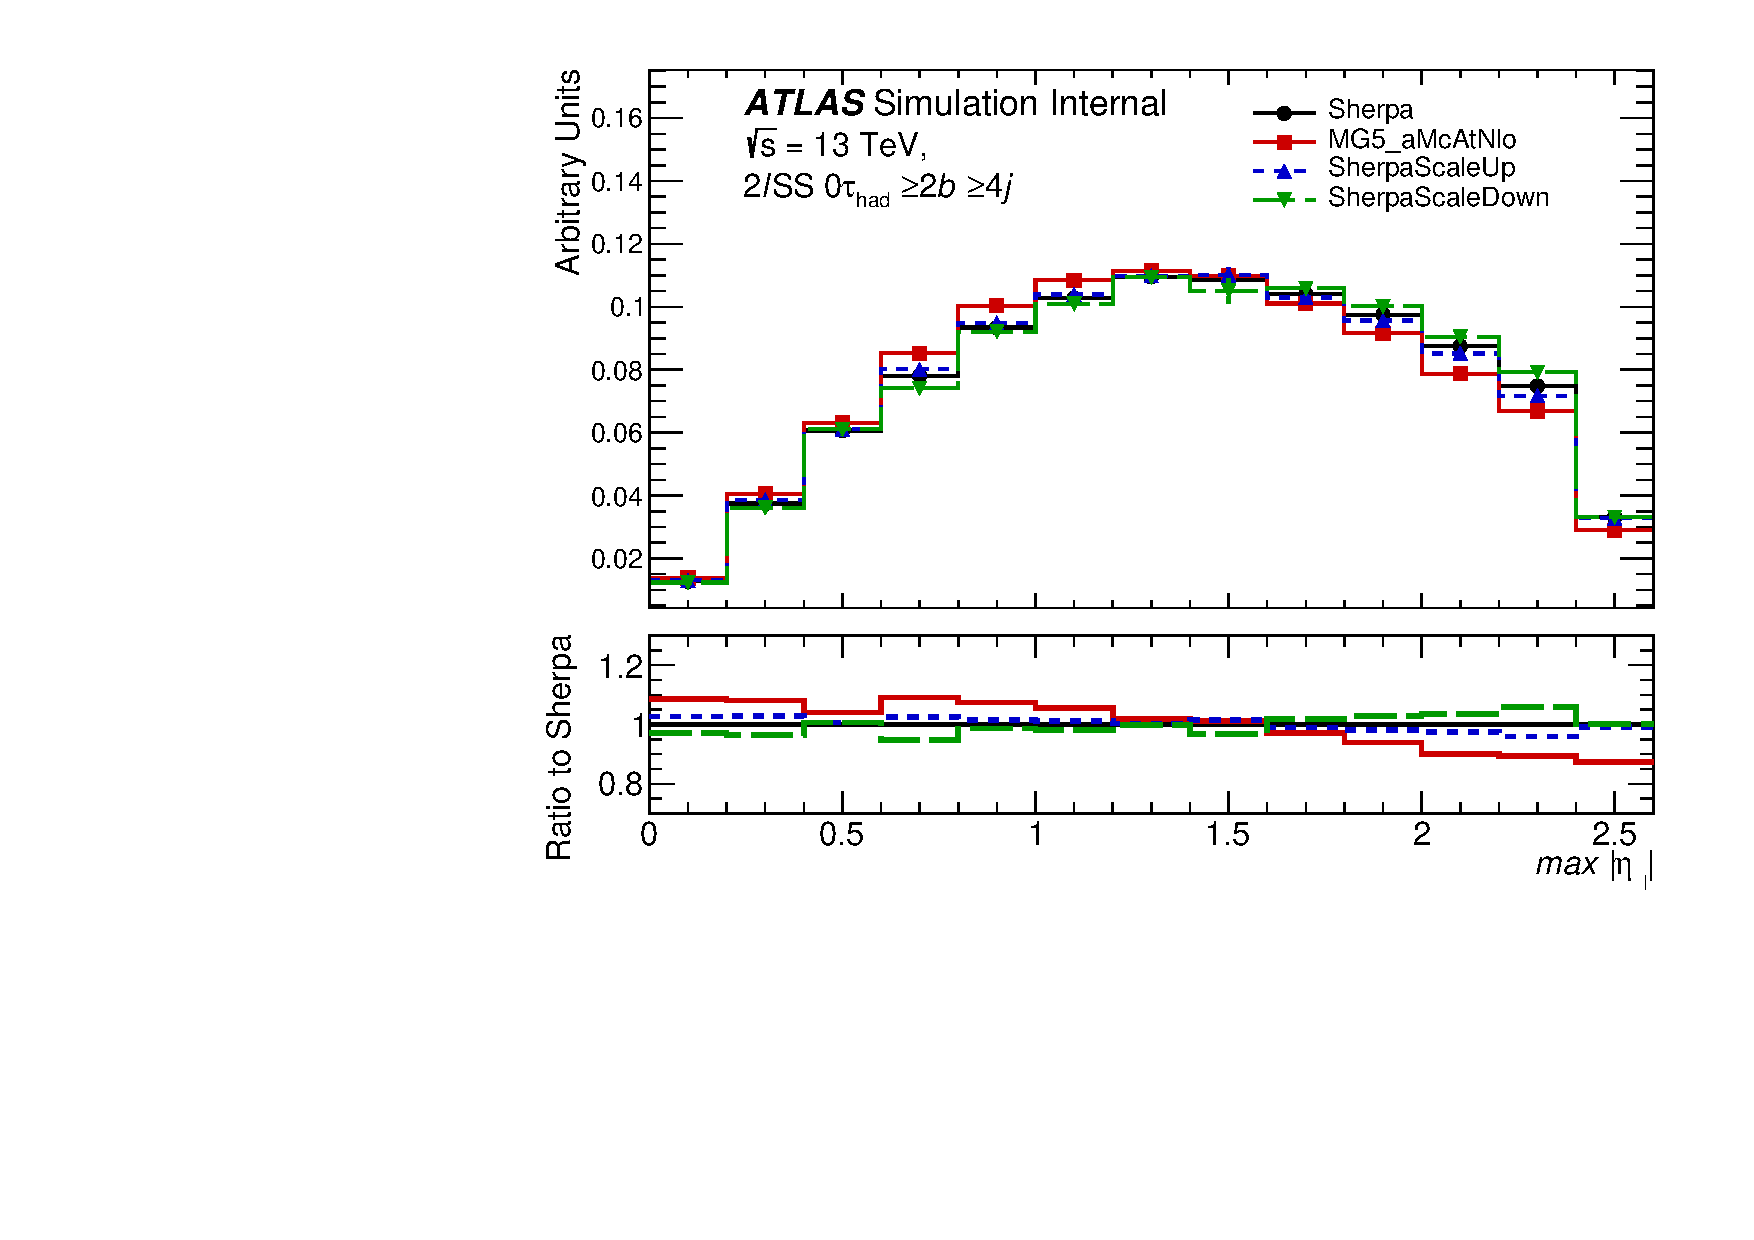
\includegraphics[width=0.45\textwidth]{Plots/ttV/shape/c_Region_1_maxEta_ll}\\
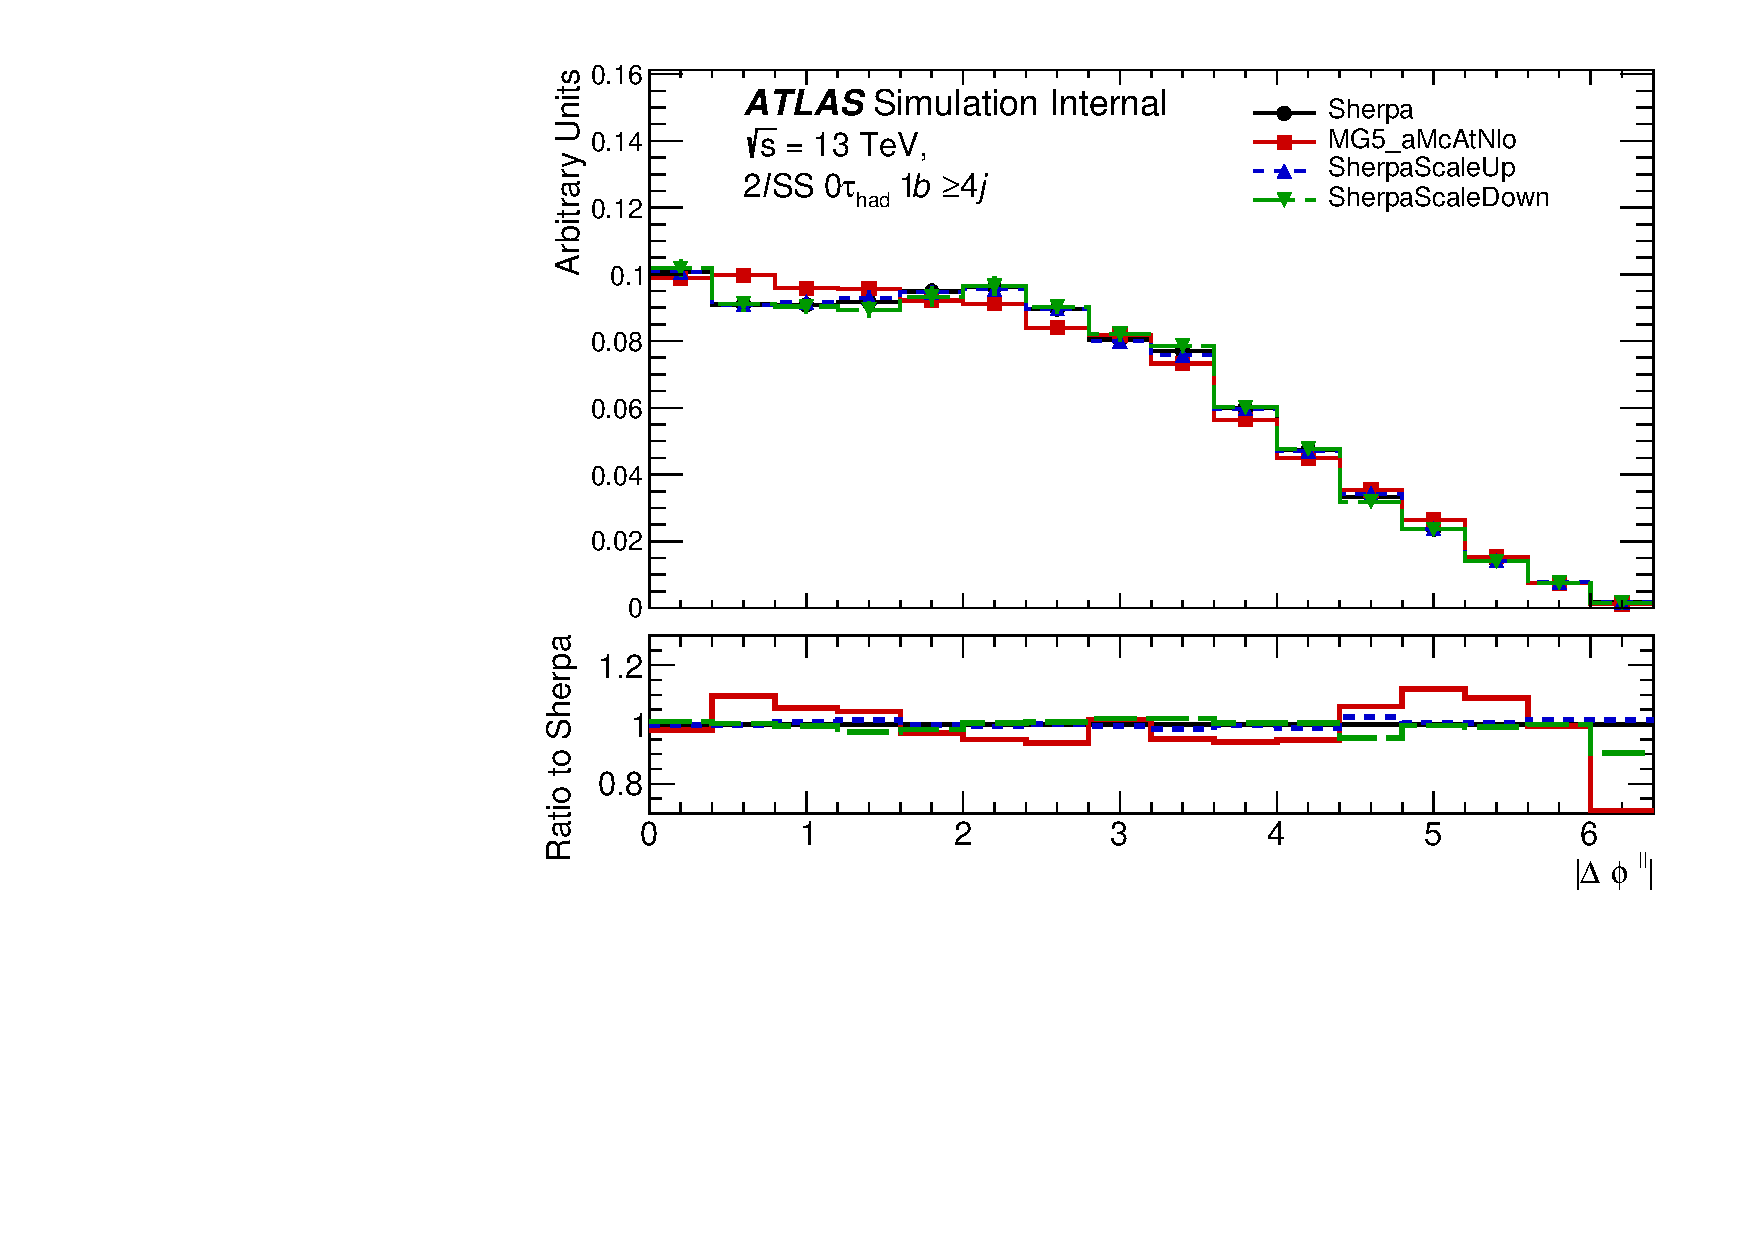
\includegraphics[width=0.45\textwidth]{Plots/ttV/shape/c_Region_0_lep_dPhi} 
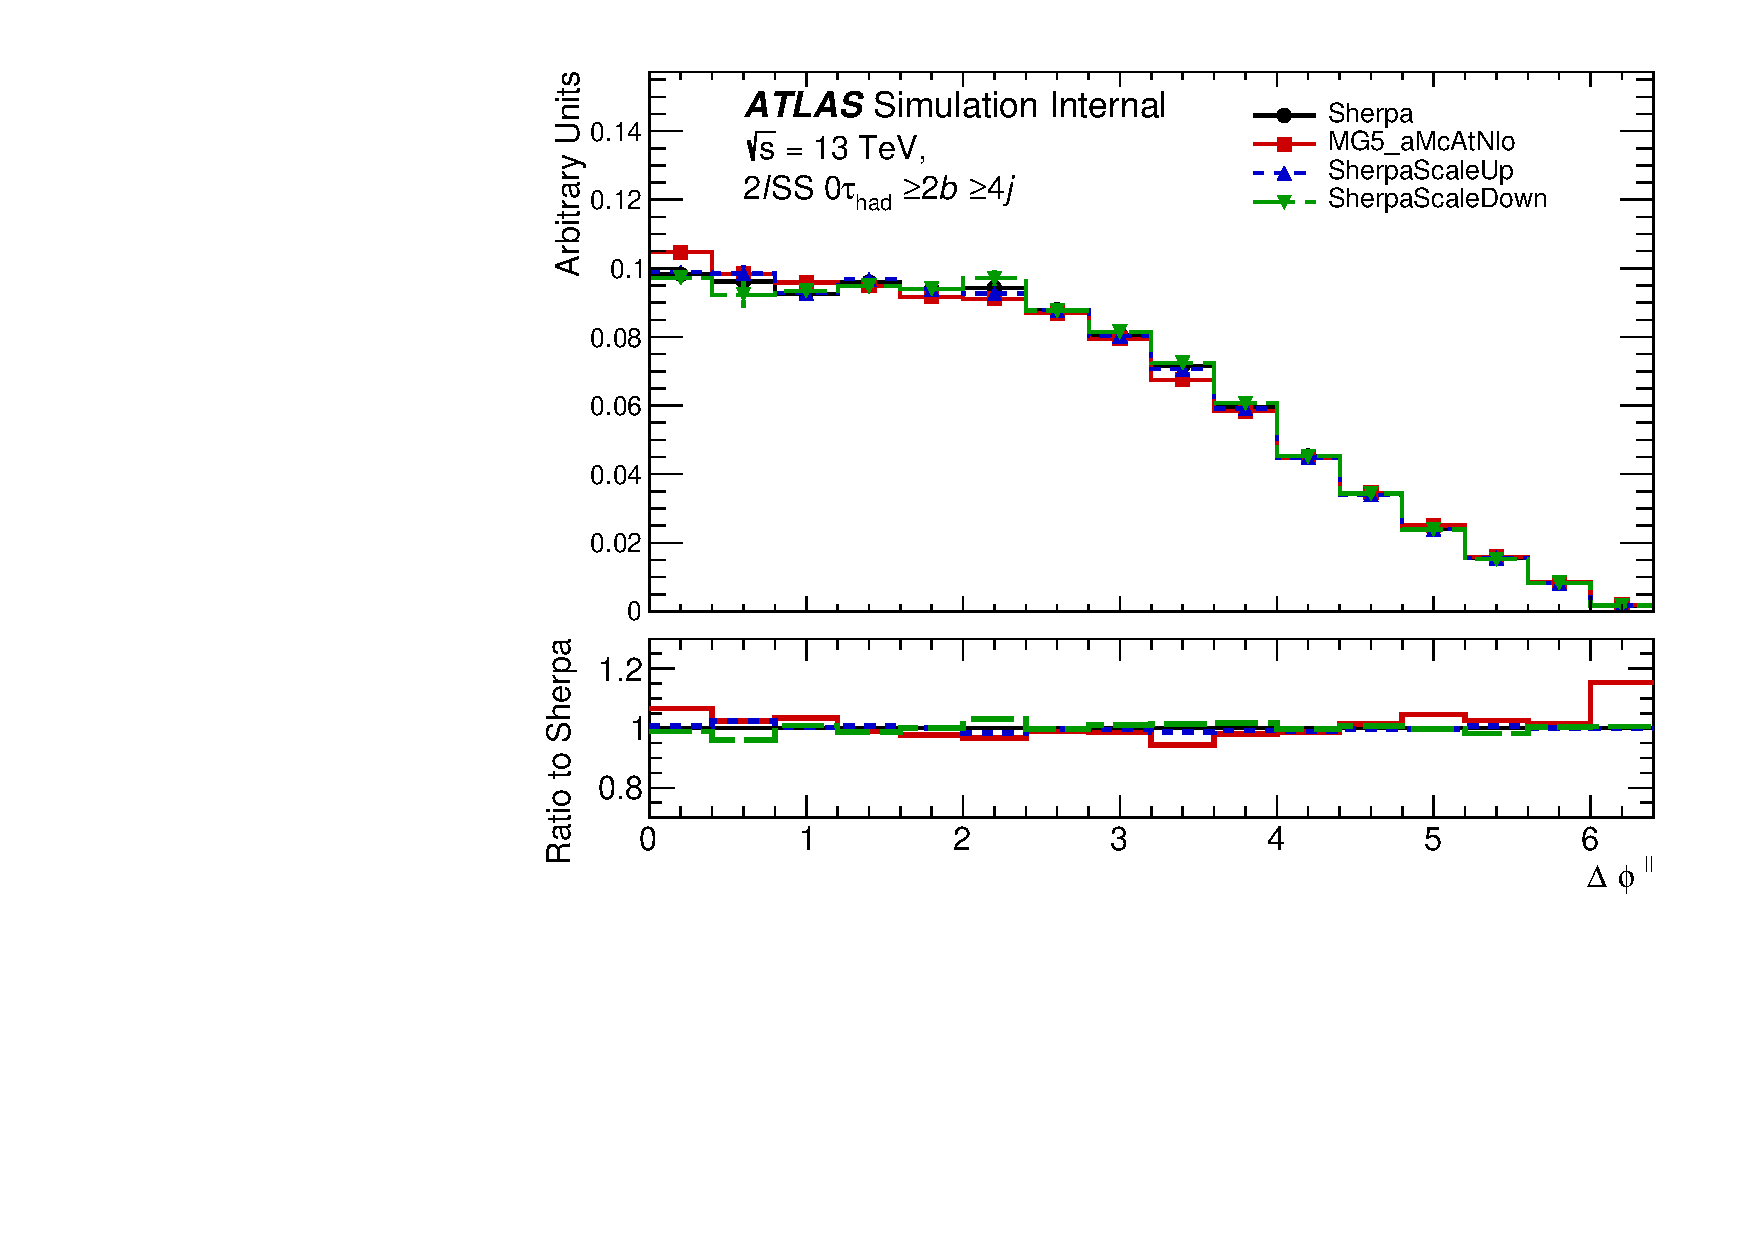
\includegraphics[width=0.45\textwidth]{Plots/ttV/shape/c_Region_1_lep_dPhi} 
  \caption{Distribution of the angular distance between the two leptons (top), maximum between lepton $|\eta_{\ell 0}|$ and $|\eta_{\ell 1}|$ (centre), azimuthal separation between the leptons $\Delta \phi _{\ell \ell }$ (bottom) , for the Region 1 with $N_{b-\mathrm{jets}}$=1 (left) and Region 2 with $N_{b-\mathrm{jets}}\geq$2(right) selection requiring four and more jets. 
   \label{ttV:ll_kin}}
\end{figure}
% 



\begin{figure}[!htb]
\centering
	% \hspace{25mm} $DRl_0l_1$  \hspace{20mm} $max|\eta^{\ell\ell}|$\\
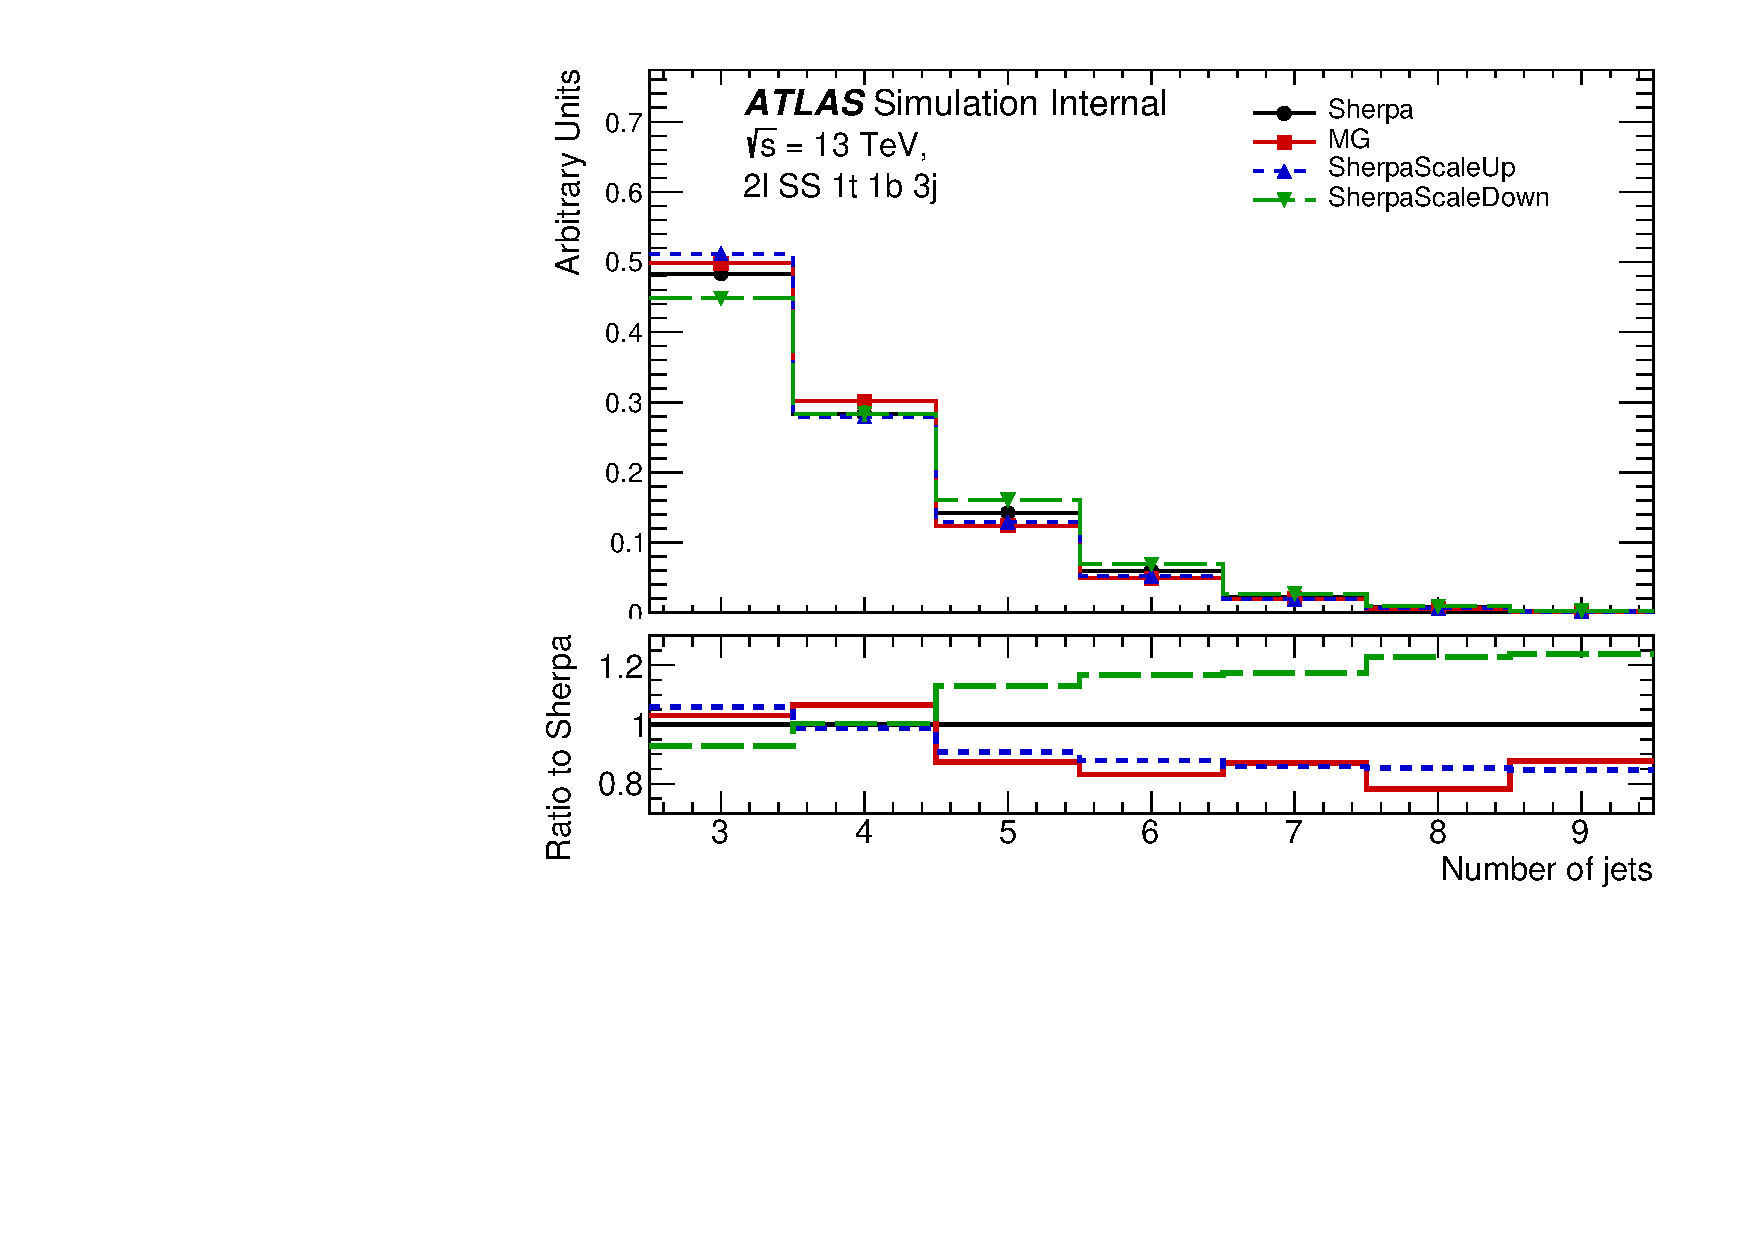
\includegraphics[width=0.45\textwidth]{Plots/ttV/shape/c_Region_4_nJets}
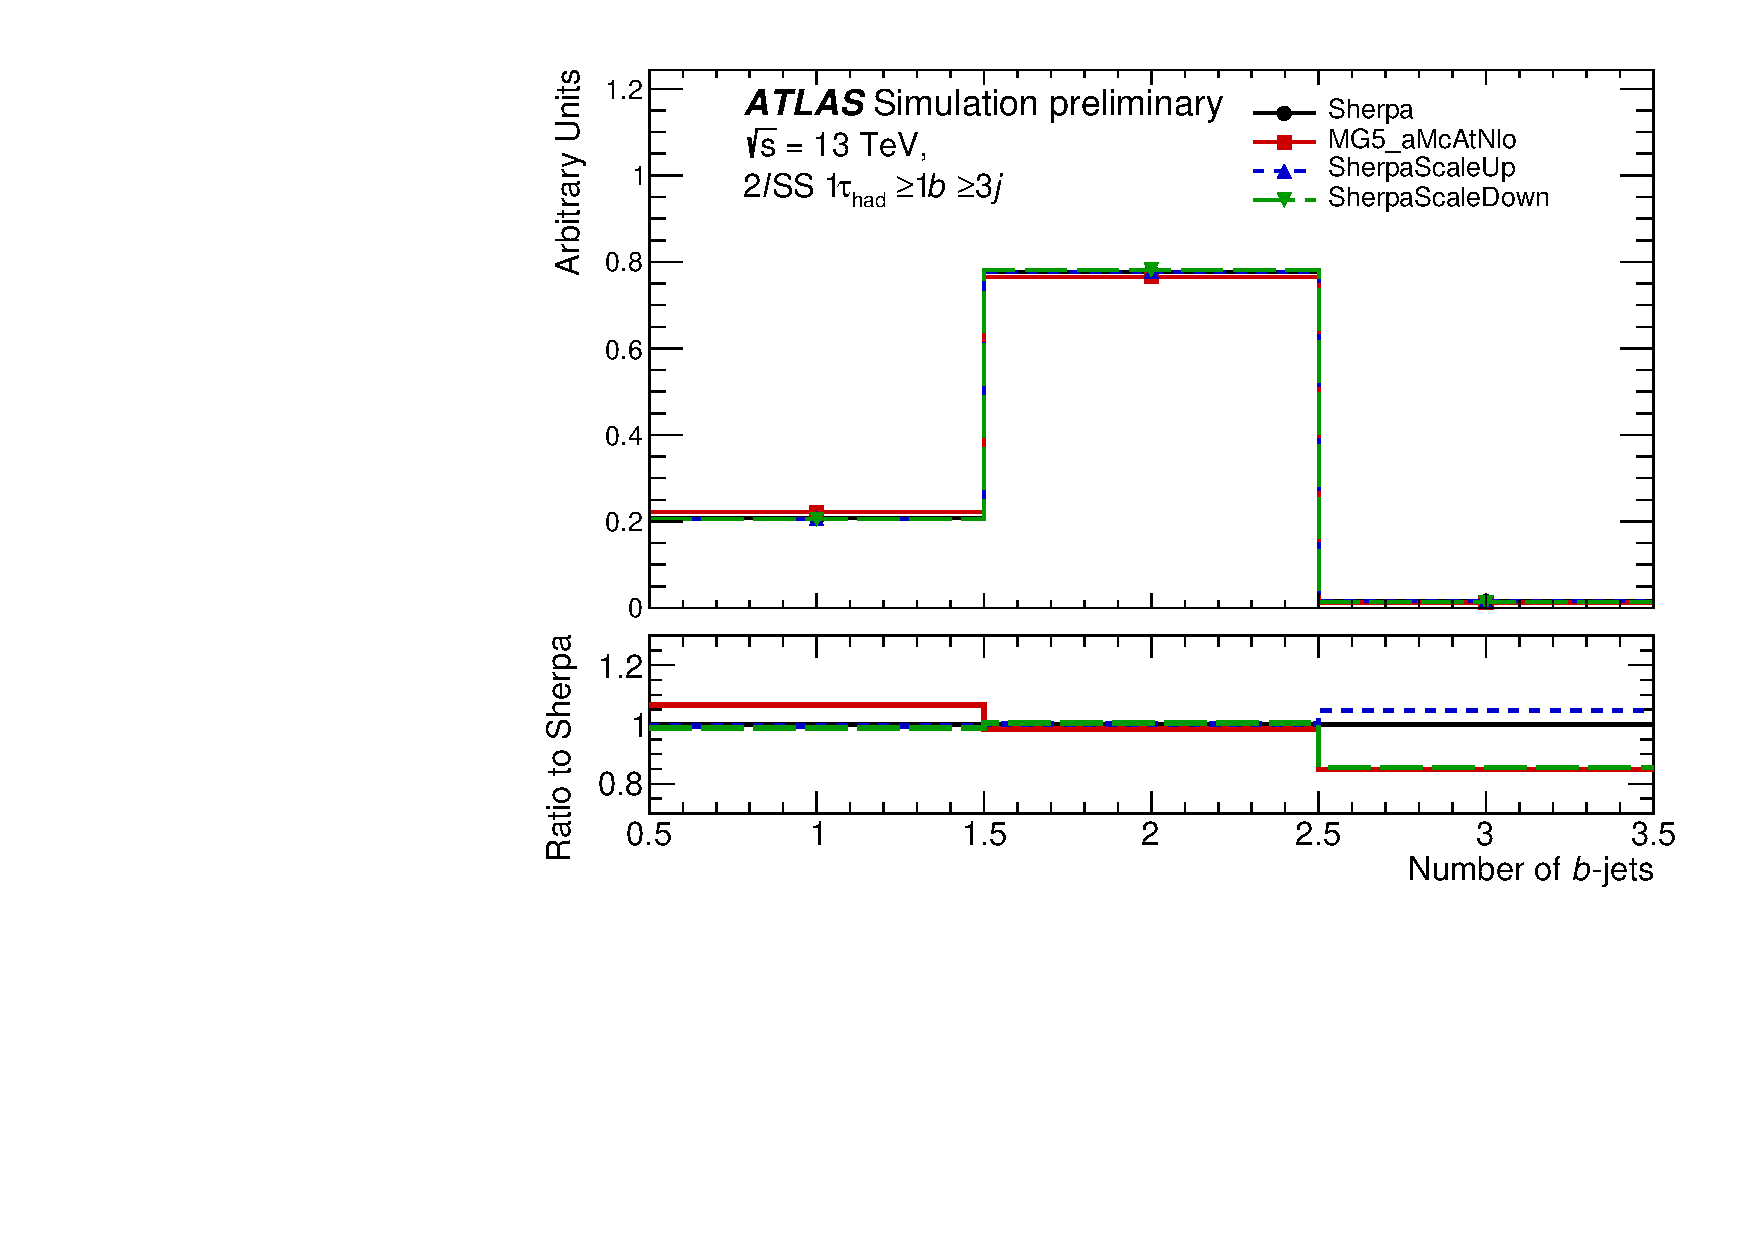
\includegraphics[width=0.45\textwidth]{Plots/ttV/shape/c_Region_4_nBtagJets}\\
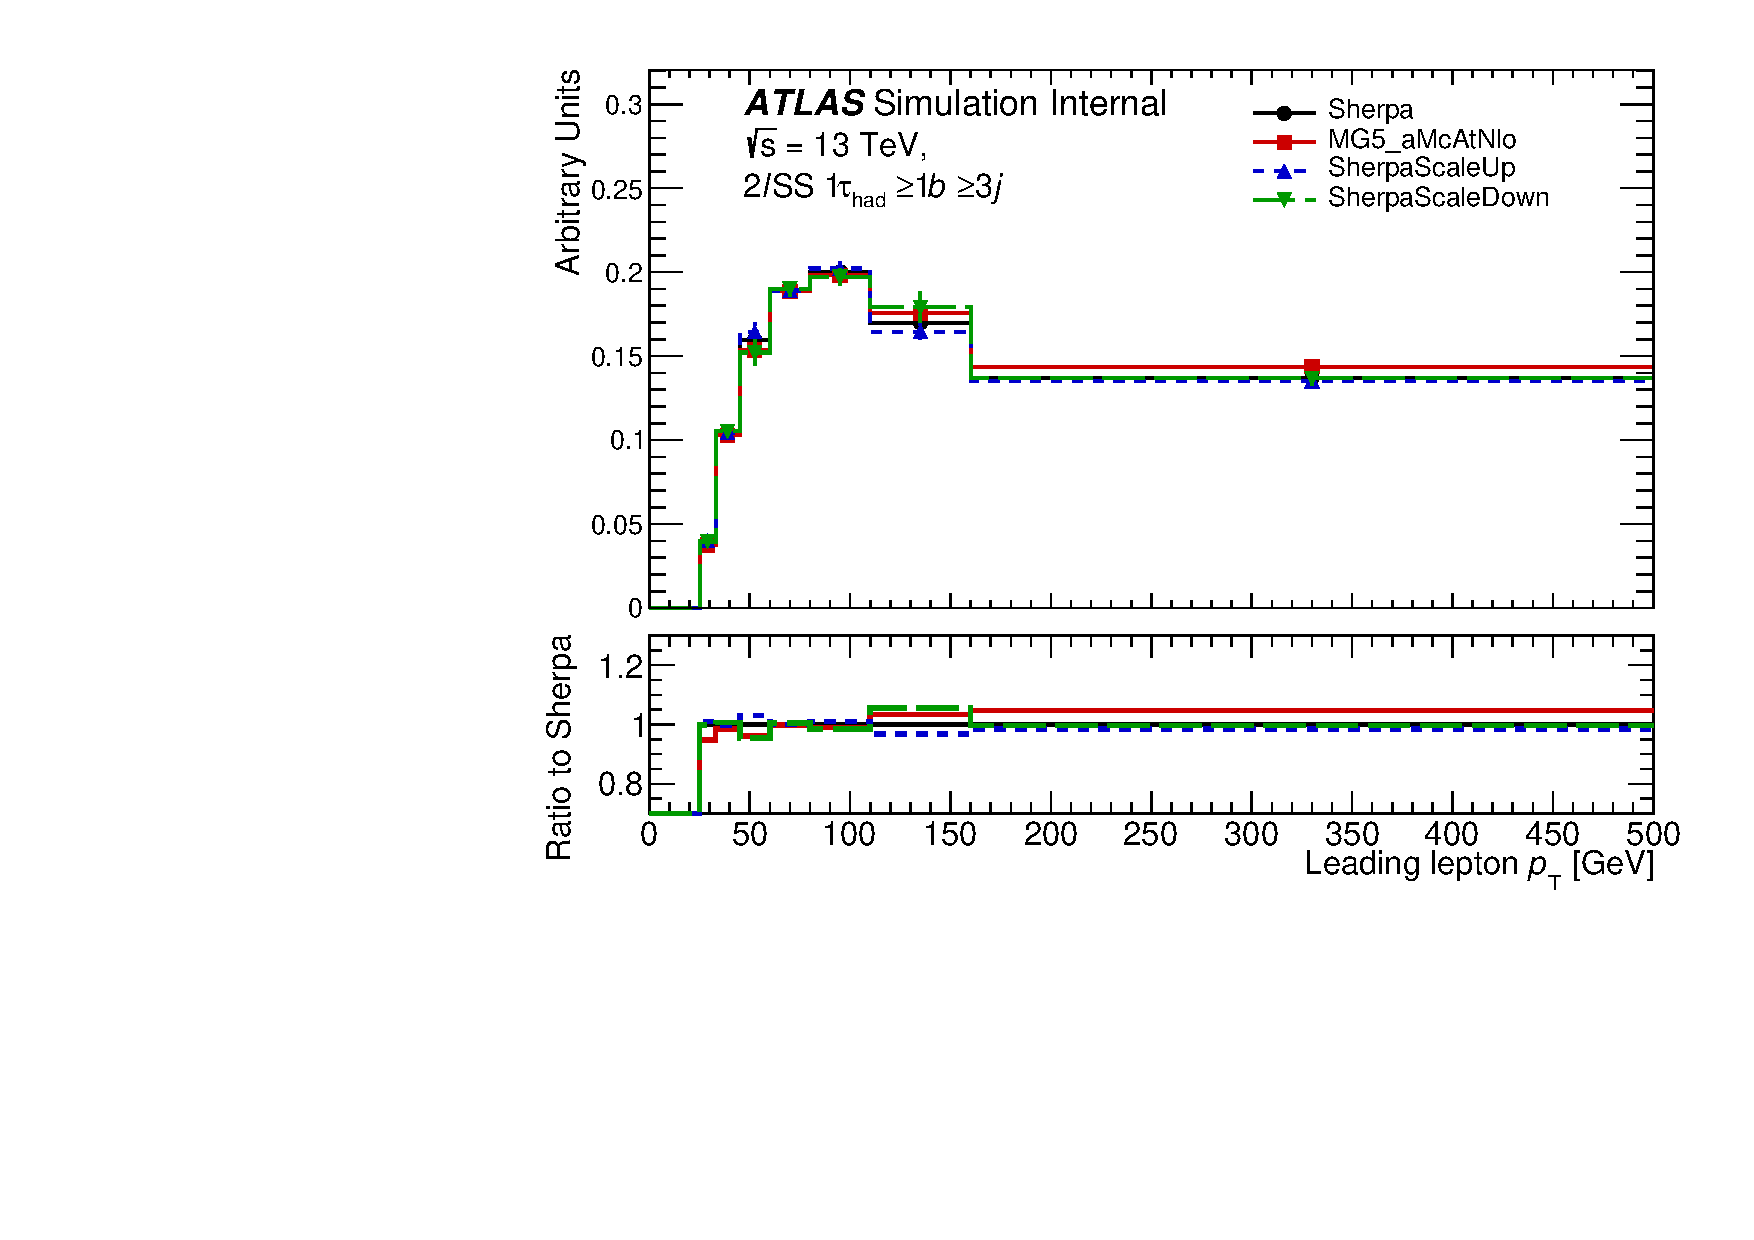
\includegraphics[width=0.45\textwidth]{Plots/ttV/shape/c_Region_4_lep_Pt_0} 
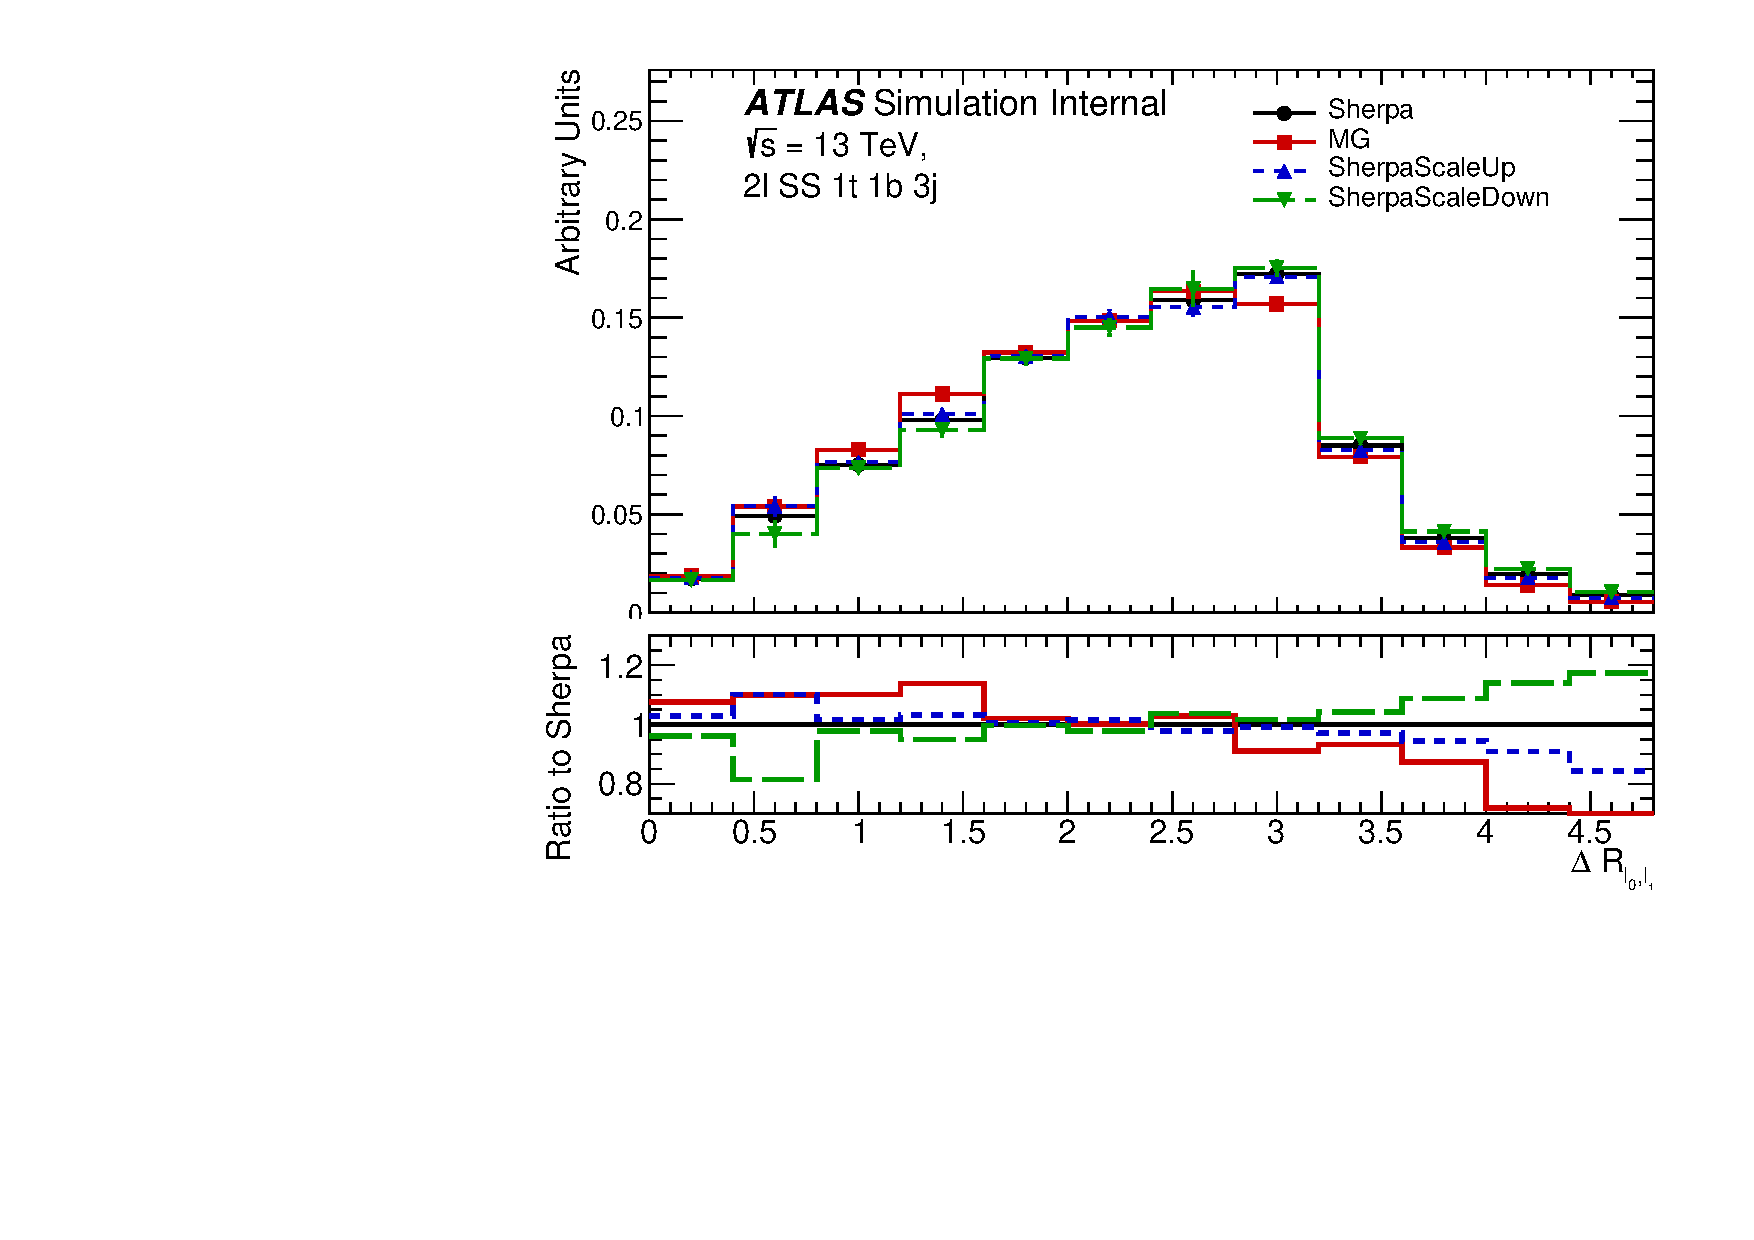
\includegraphics[width=0.45\textwidth]{Plots/ttV/shape/c_Region_4_DRll01}\\
  \caption{Distribution of the the jet multiplicity, number of $b$-jets, the leading lepton transverse momentum and the angular distance between the two leptons  $\Delta R _{\ell \ell }$ for the Region 5 with 1$\tau_{had}$ selection. 
   \label{ttV:tauR_kin}}
\end{figure}
% 



%
%
%
%%
%
%
\subsubsection{Generator comparison}
\label{sec:ttw_gen}

In the following section a comparison of the generators will be given in terms of fiducial cross section. Some difference is observed in $\sigma_{fid}^{gen}=A_X^{gen}\times \sigma_{tot}^{gen}$ , where $A_X^{gen}$ is the acceptance factor of particular region, $\sigma_{tot}^{gen}$ is the total generator cross section (taken directly from generation - i.e. not including any correction factors). The cross sections are $\sigma_{tot}^{Sherpa}=652$~fb and $\sigma_{tot}^{MG5\_aMcAtNlo}=548$~fb for Sherpa and MG5\_aMcAtNlo correspondingly. The fiducial cross sections of the five regions defined in Section~\ref{sec:ttw_fid} are presented on Figure~\ref{ttV:fid_xs}.
The same set of distribution discussed in Section~\ref{sec:ttw_shape} is presented, normalised to the fiducial cross section in Figures~\ref{ttV:den_4j12b}-\ref{ttV:den_tauR_kin}.

\begin{figure}[!htb]
\centering
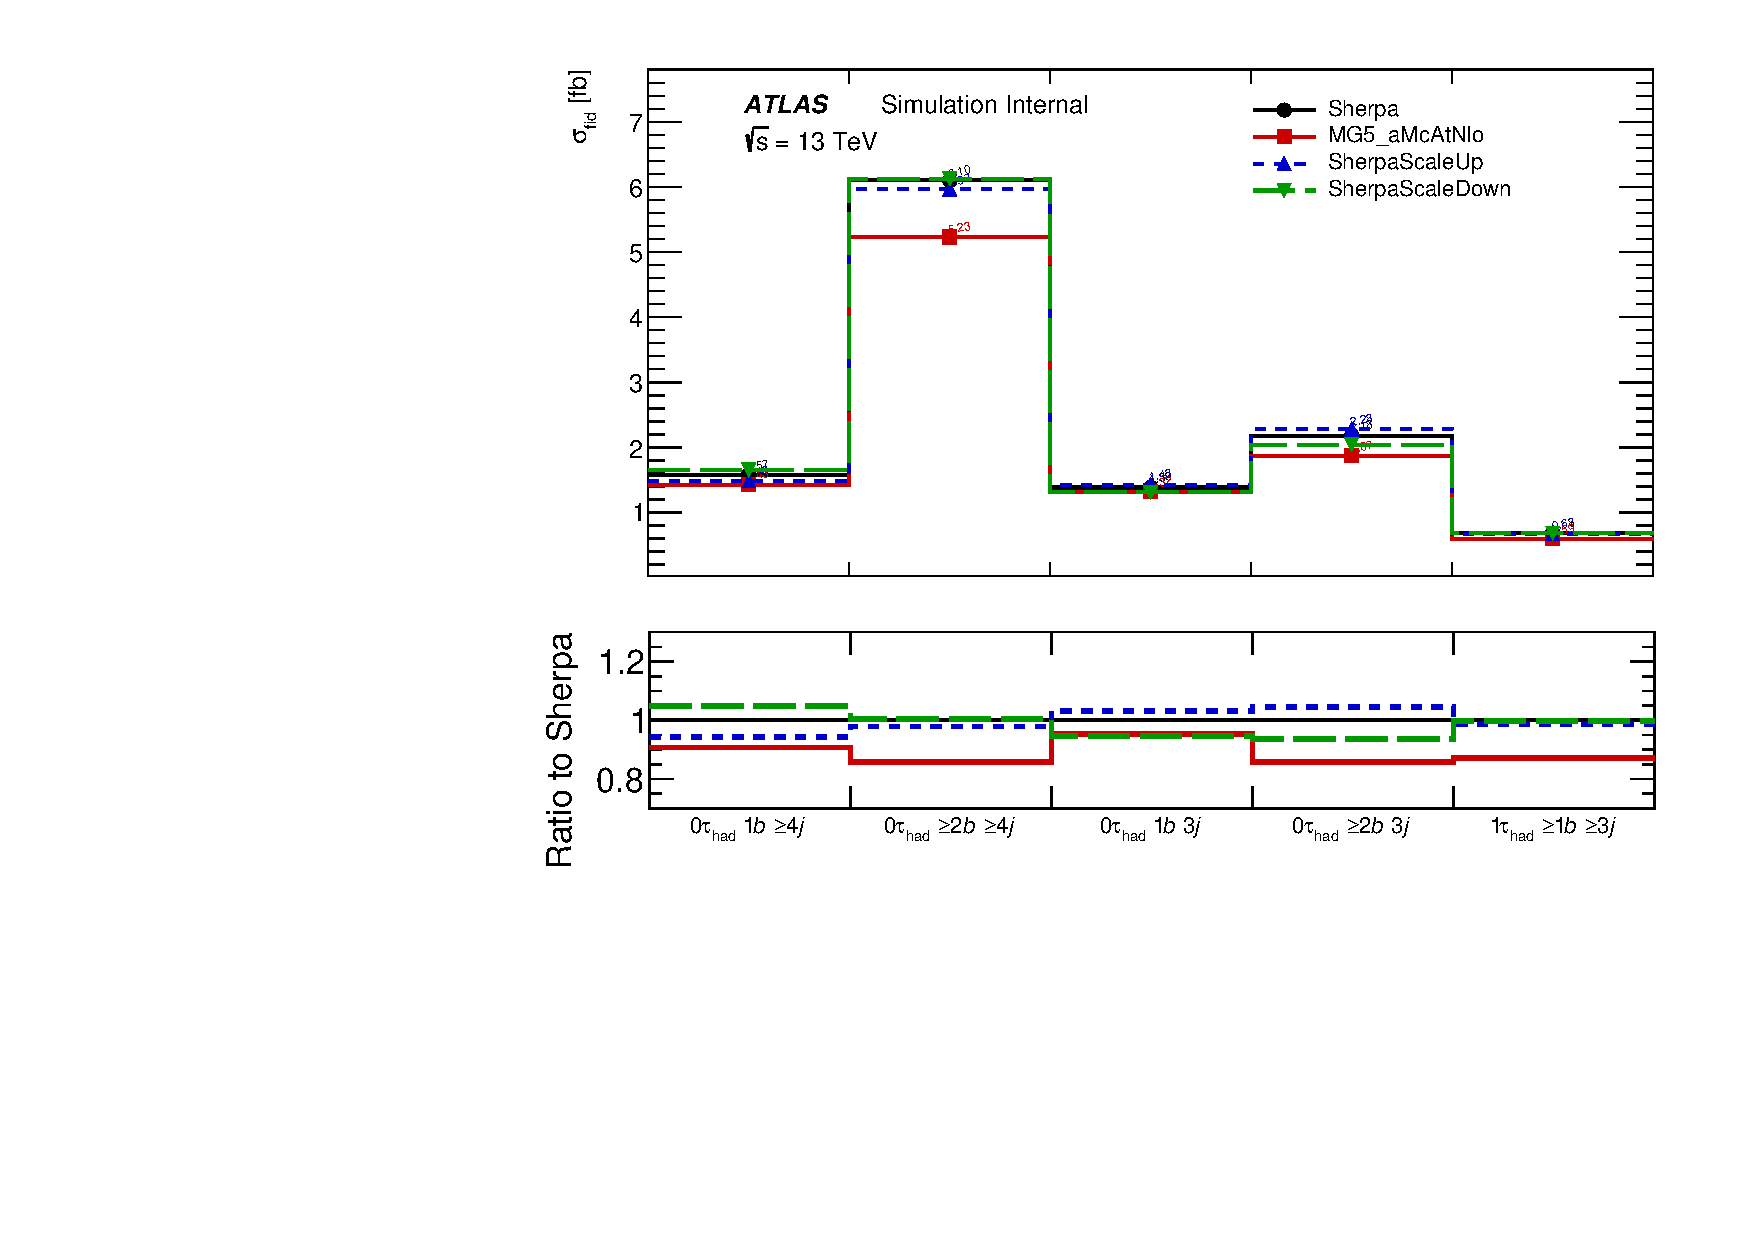
\includegraphics[width=0.45\textwidth]{Plots/ttV/generator/acc_7f}
  \caption{The fiducial cross sections, $\sigma_{fid}^{gen}=A_X^{gen}\times \sigma_{tot}^{gen}$,  of the five regions for $ttW$ analysis. \label{ttV:fid_xs}}
\end{figure}


\begin{figure}[!htb]
\centering
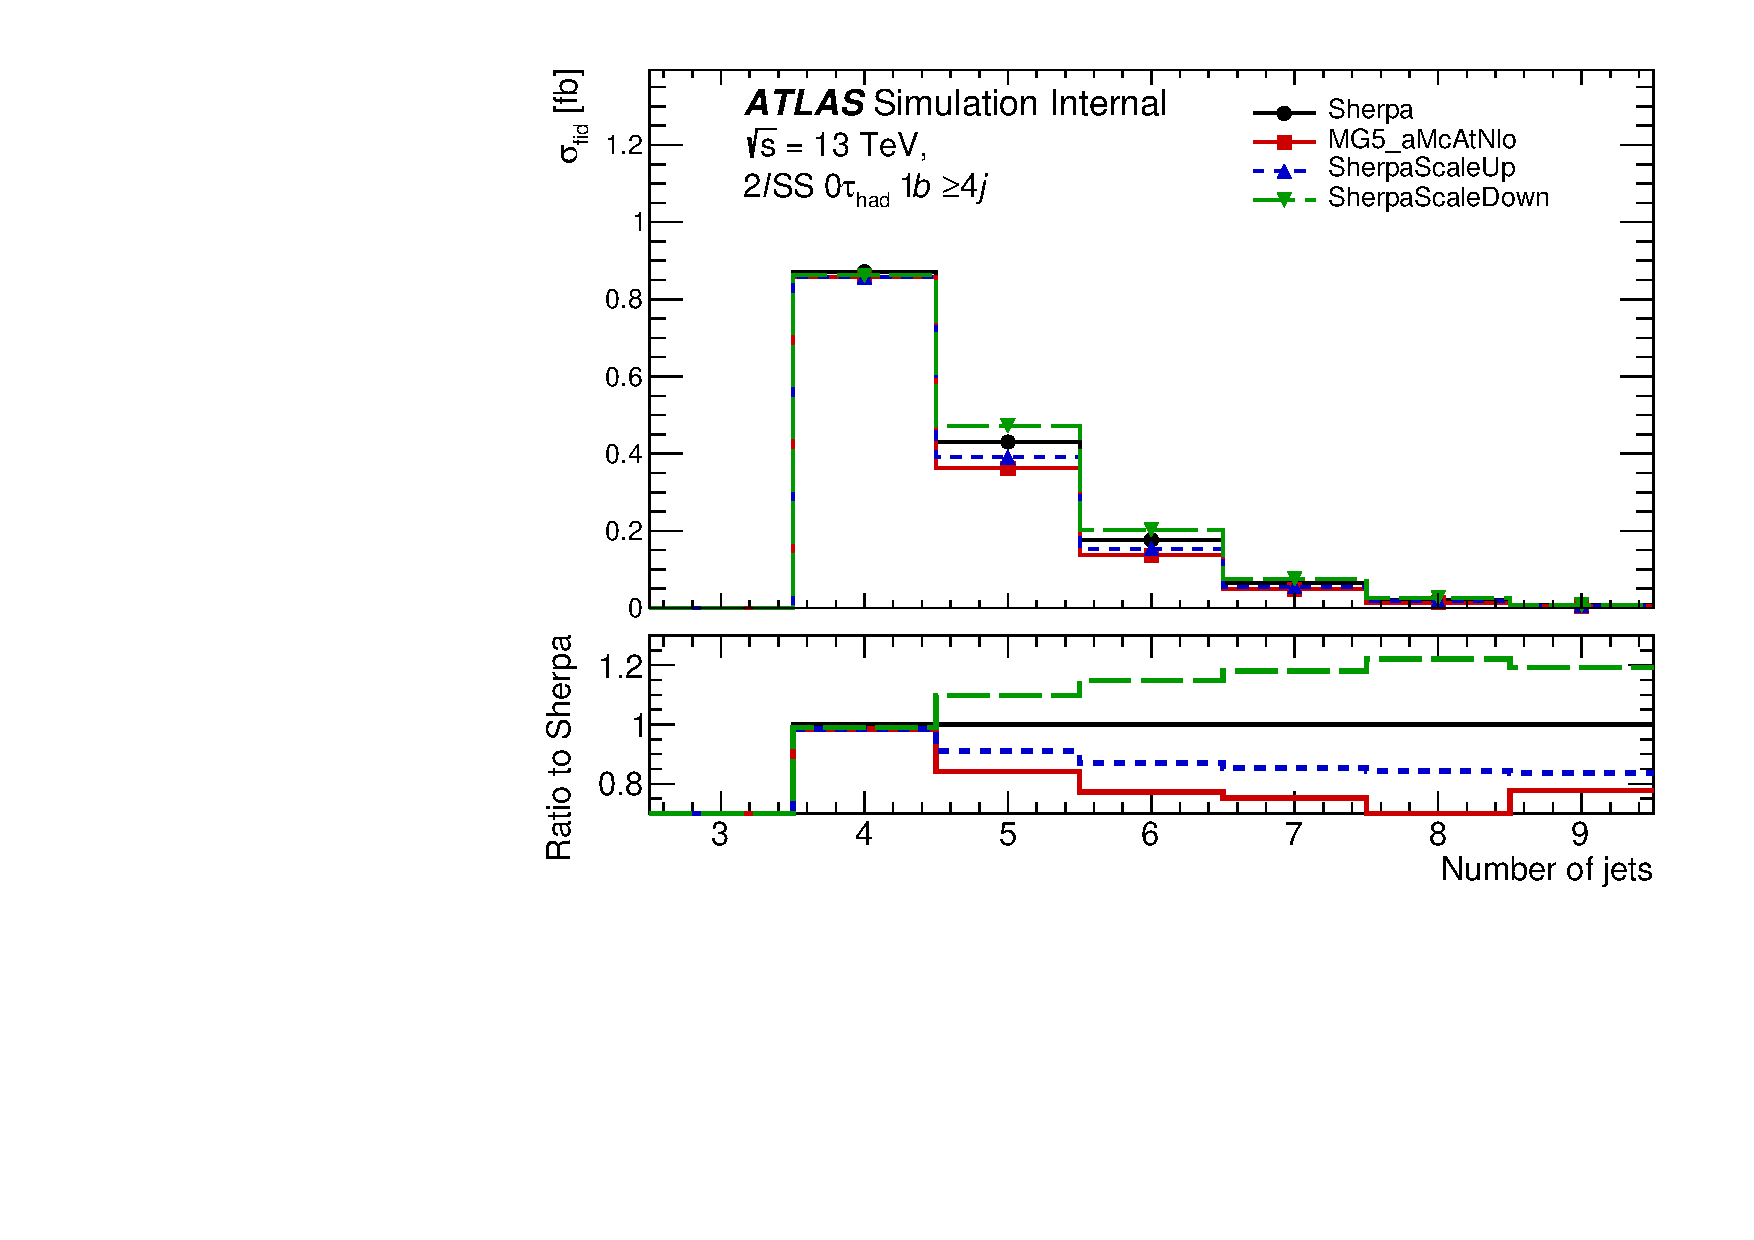
\includegraphics[width=0.45\textwidth]{Plots/ttV/generator/c_Region_0_nJets}
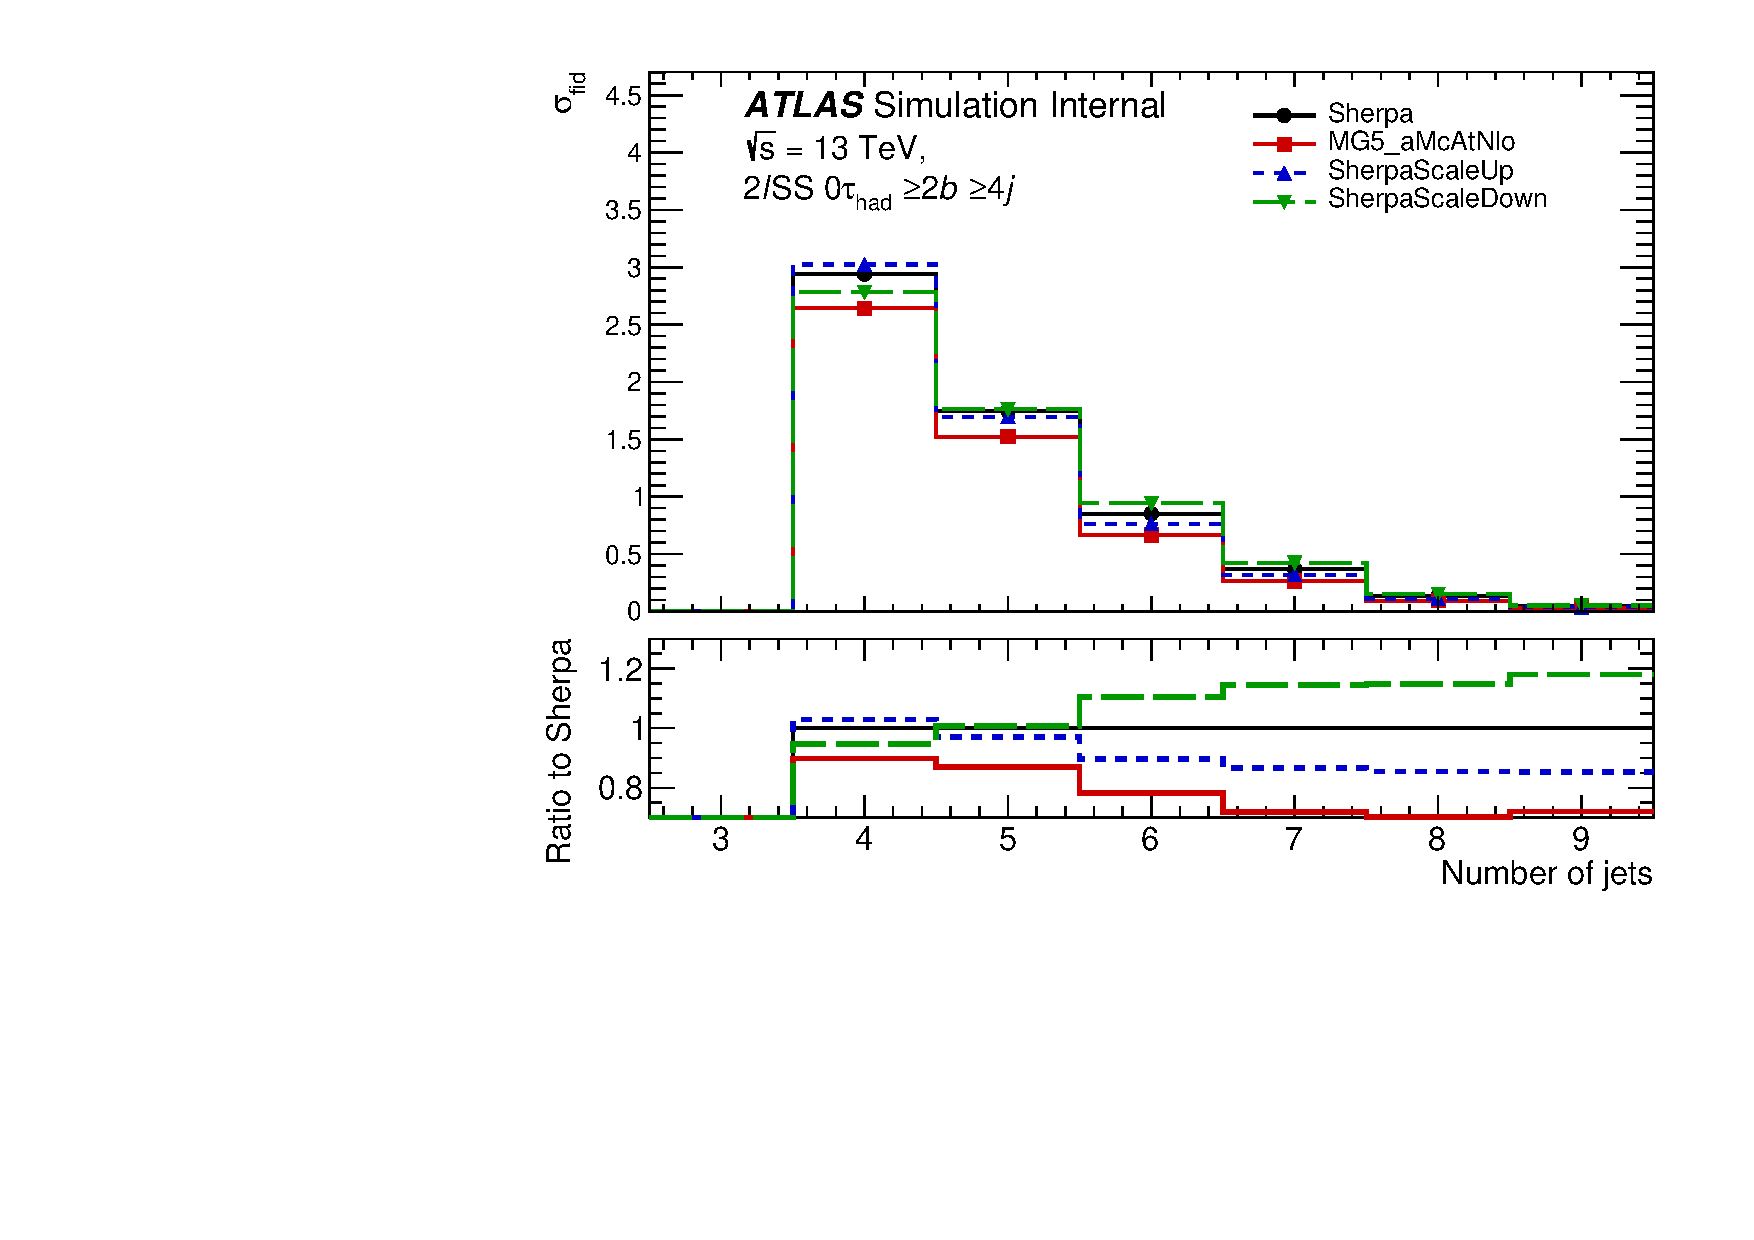
\includegraphics[width=0.45\textwidth]{Plots/ttV/generator/c_Region_1_nJets}\\
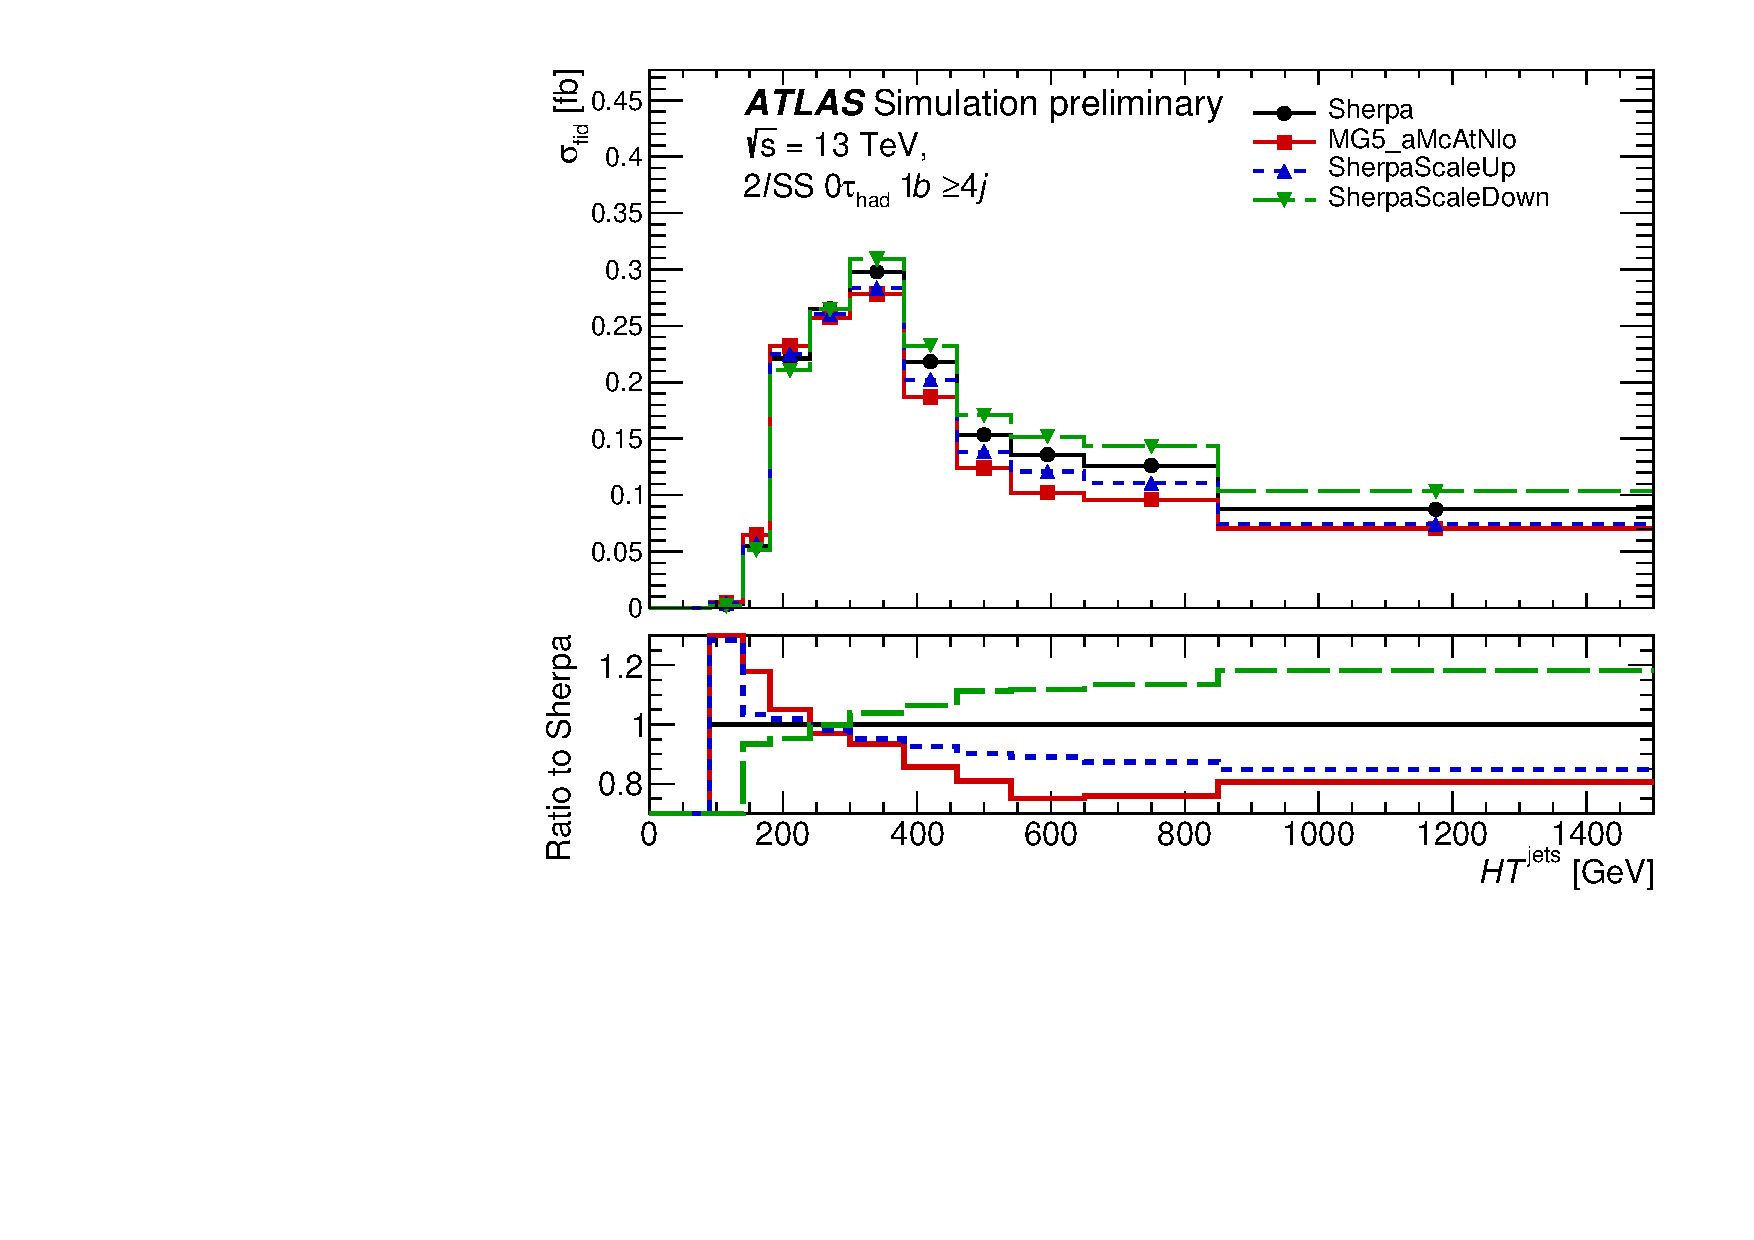
\includegraphics[width=0.45\textwidth]{Plots/ttV/generator/c_Region_0_HT_jets}
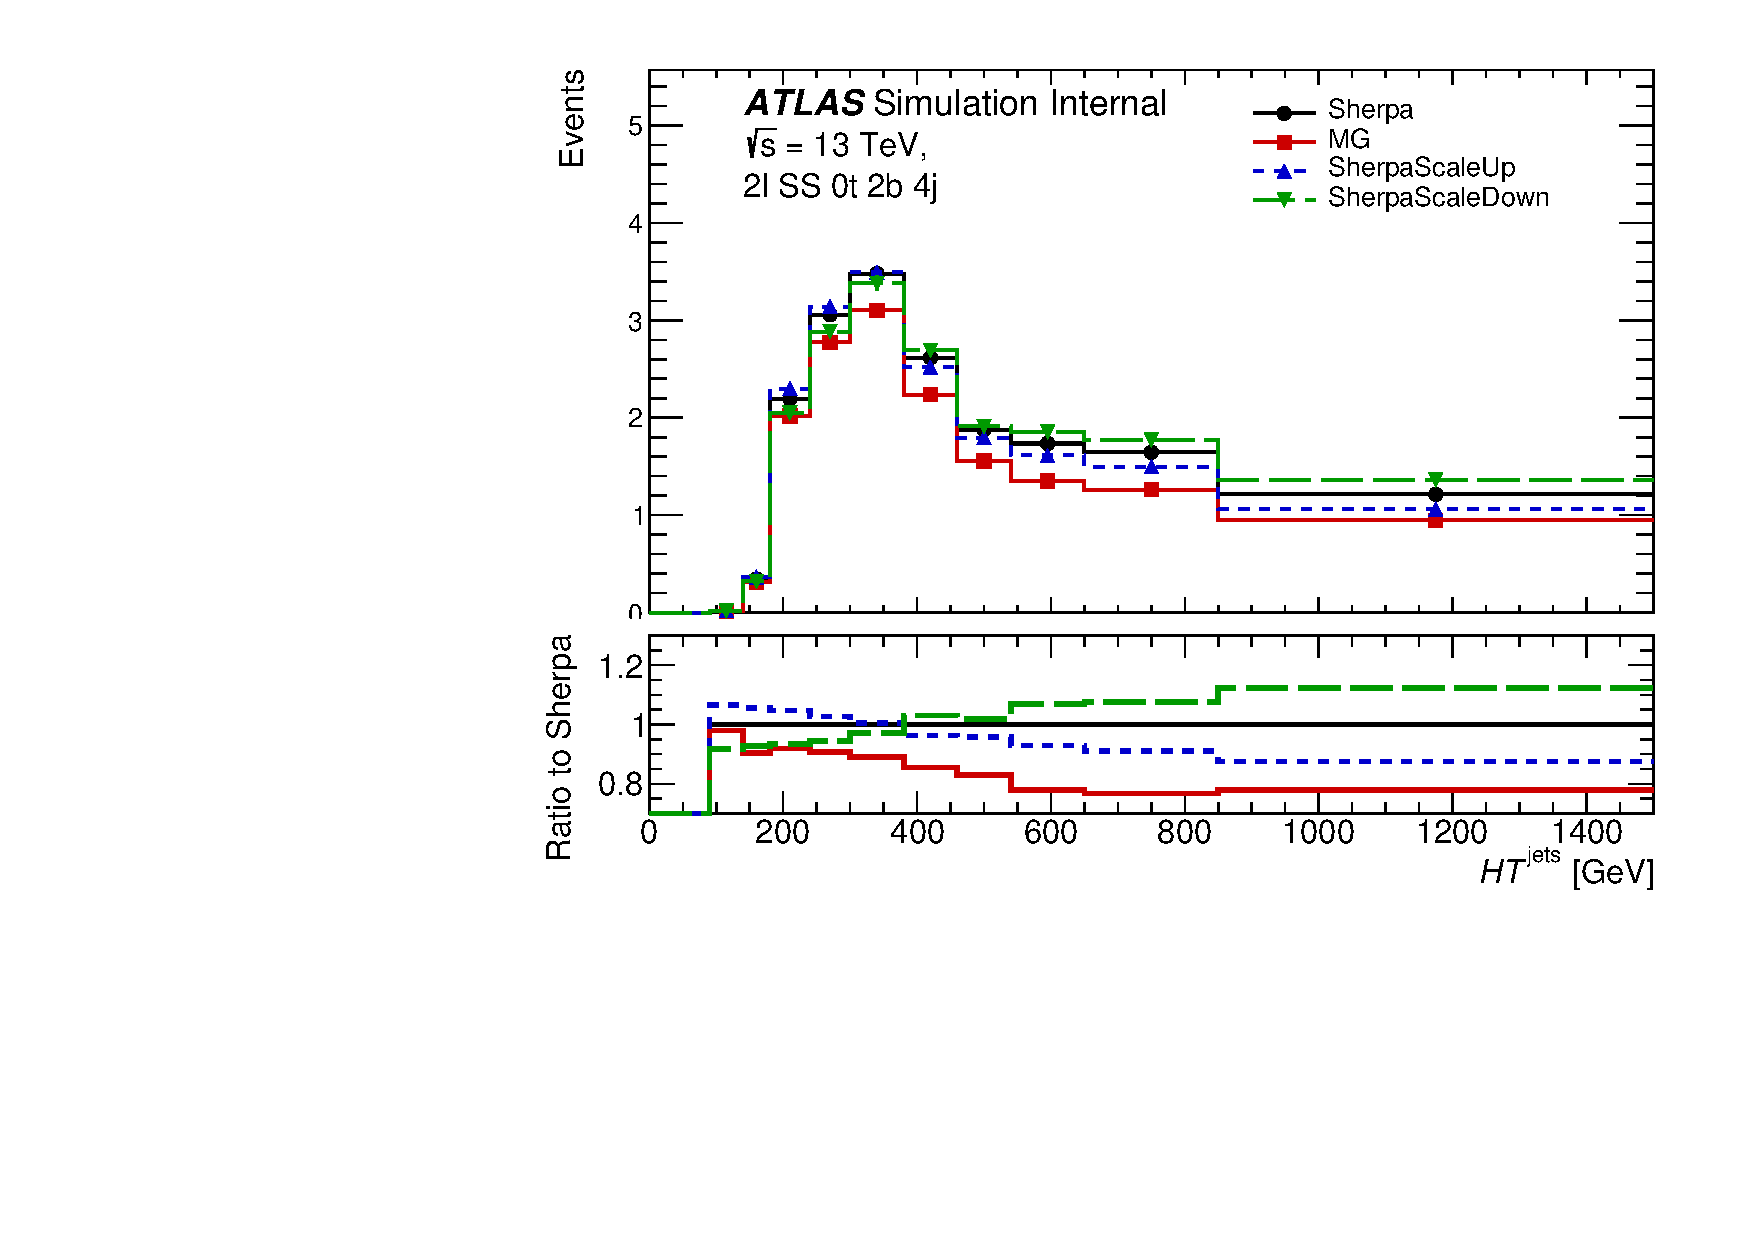
\includegraphics[width=0.45\textwidth]{Plots/ttV/generator/c_Region_1_HT_jets}\\
  \caption{Distribution of the jet multiplicities (top) and the scalar sum of jets transverse momentum, $HT^{\text{jets}}$ (bottom), for the Region 1 with $N_{b-\mathrm{jets}}$=1 (left) and Region 2 with $N_{b-\mathrm{jets}}\geq$2 (right) selection requiring four and more jets.  \label{ttV:den_4j12b}}
\end{figure}


\begin{figure}[!htb]
\centering
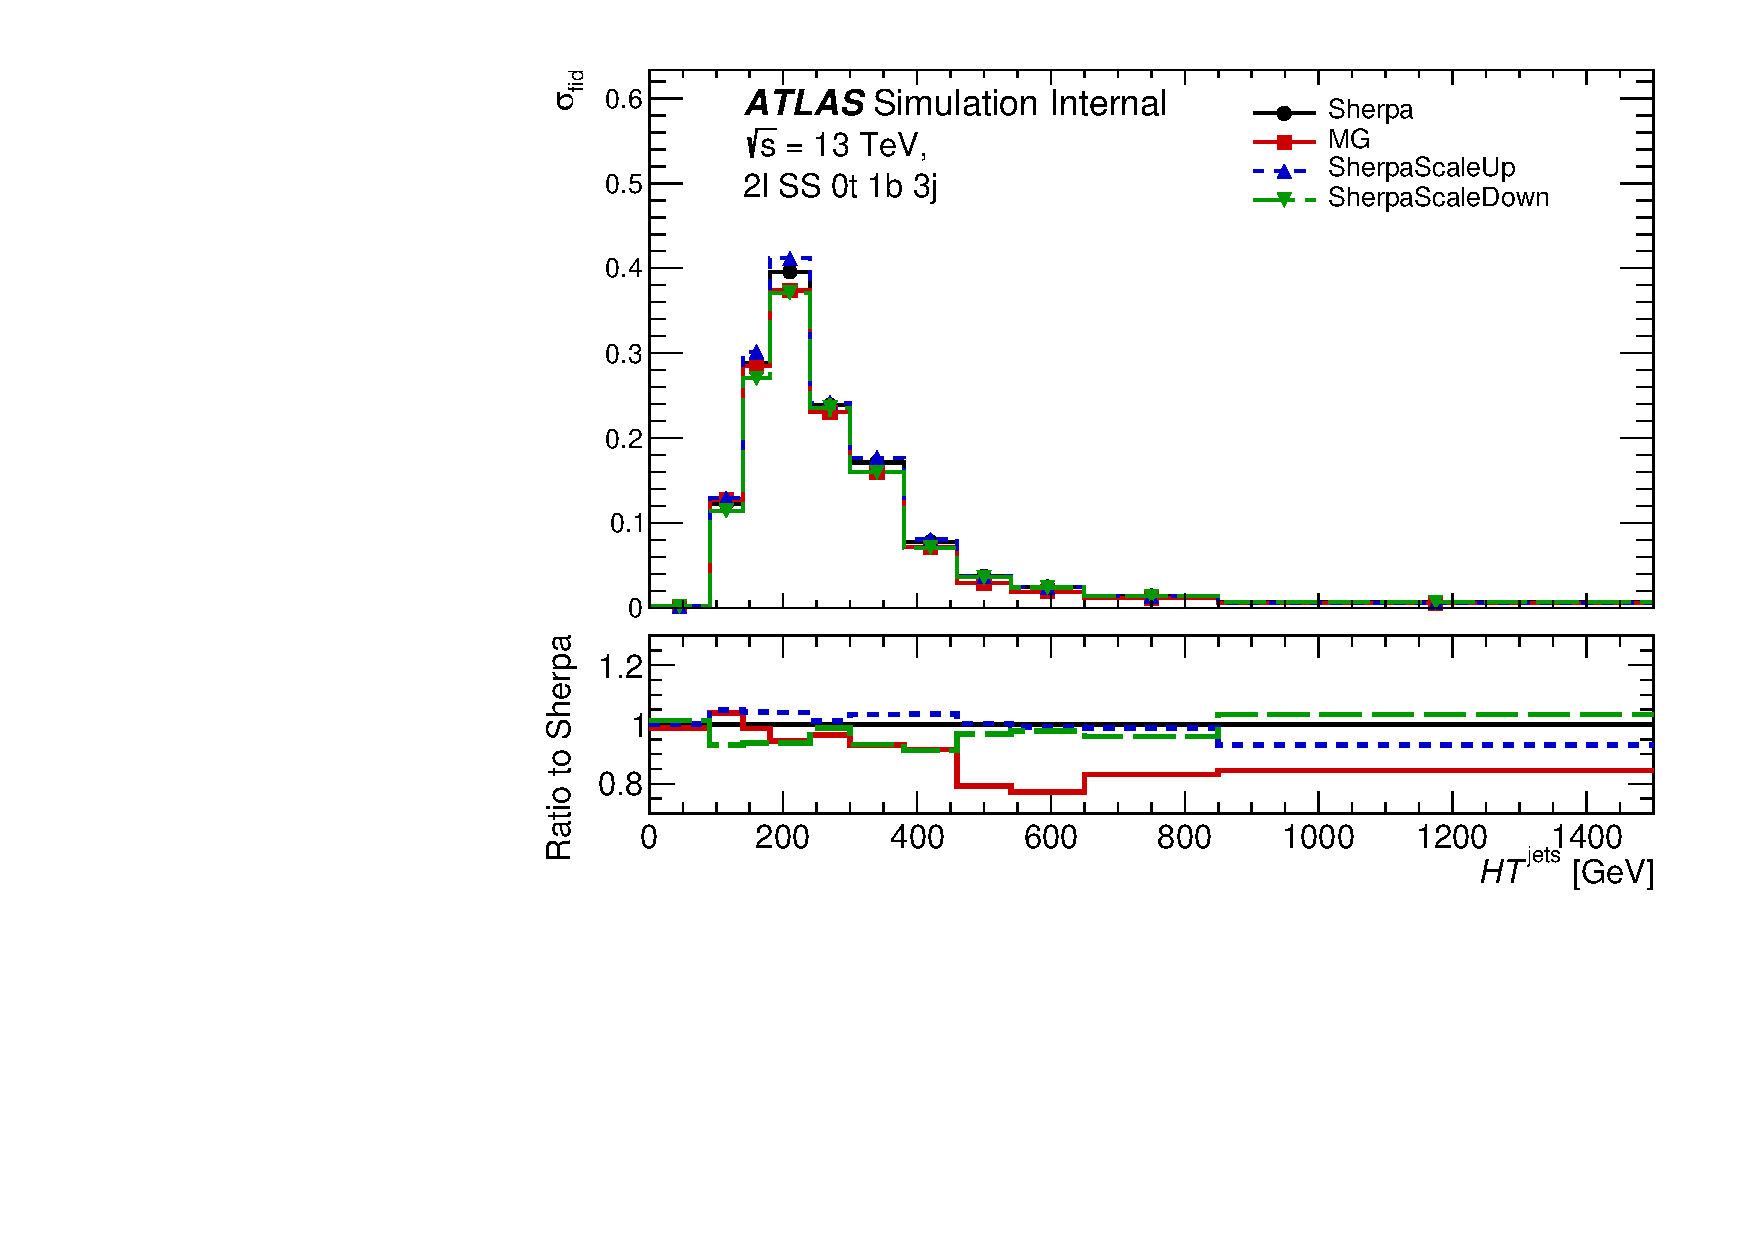
\includegraphics[width=0.45\textwidth]{Plots/ttV/generator/c_Region_2_HT_jets}
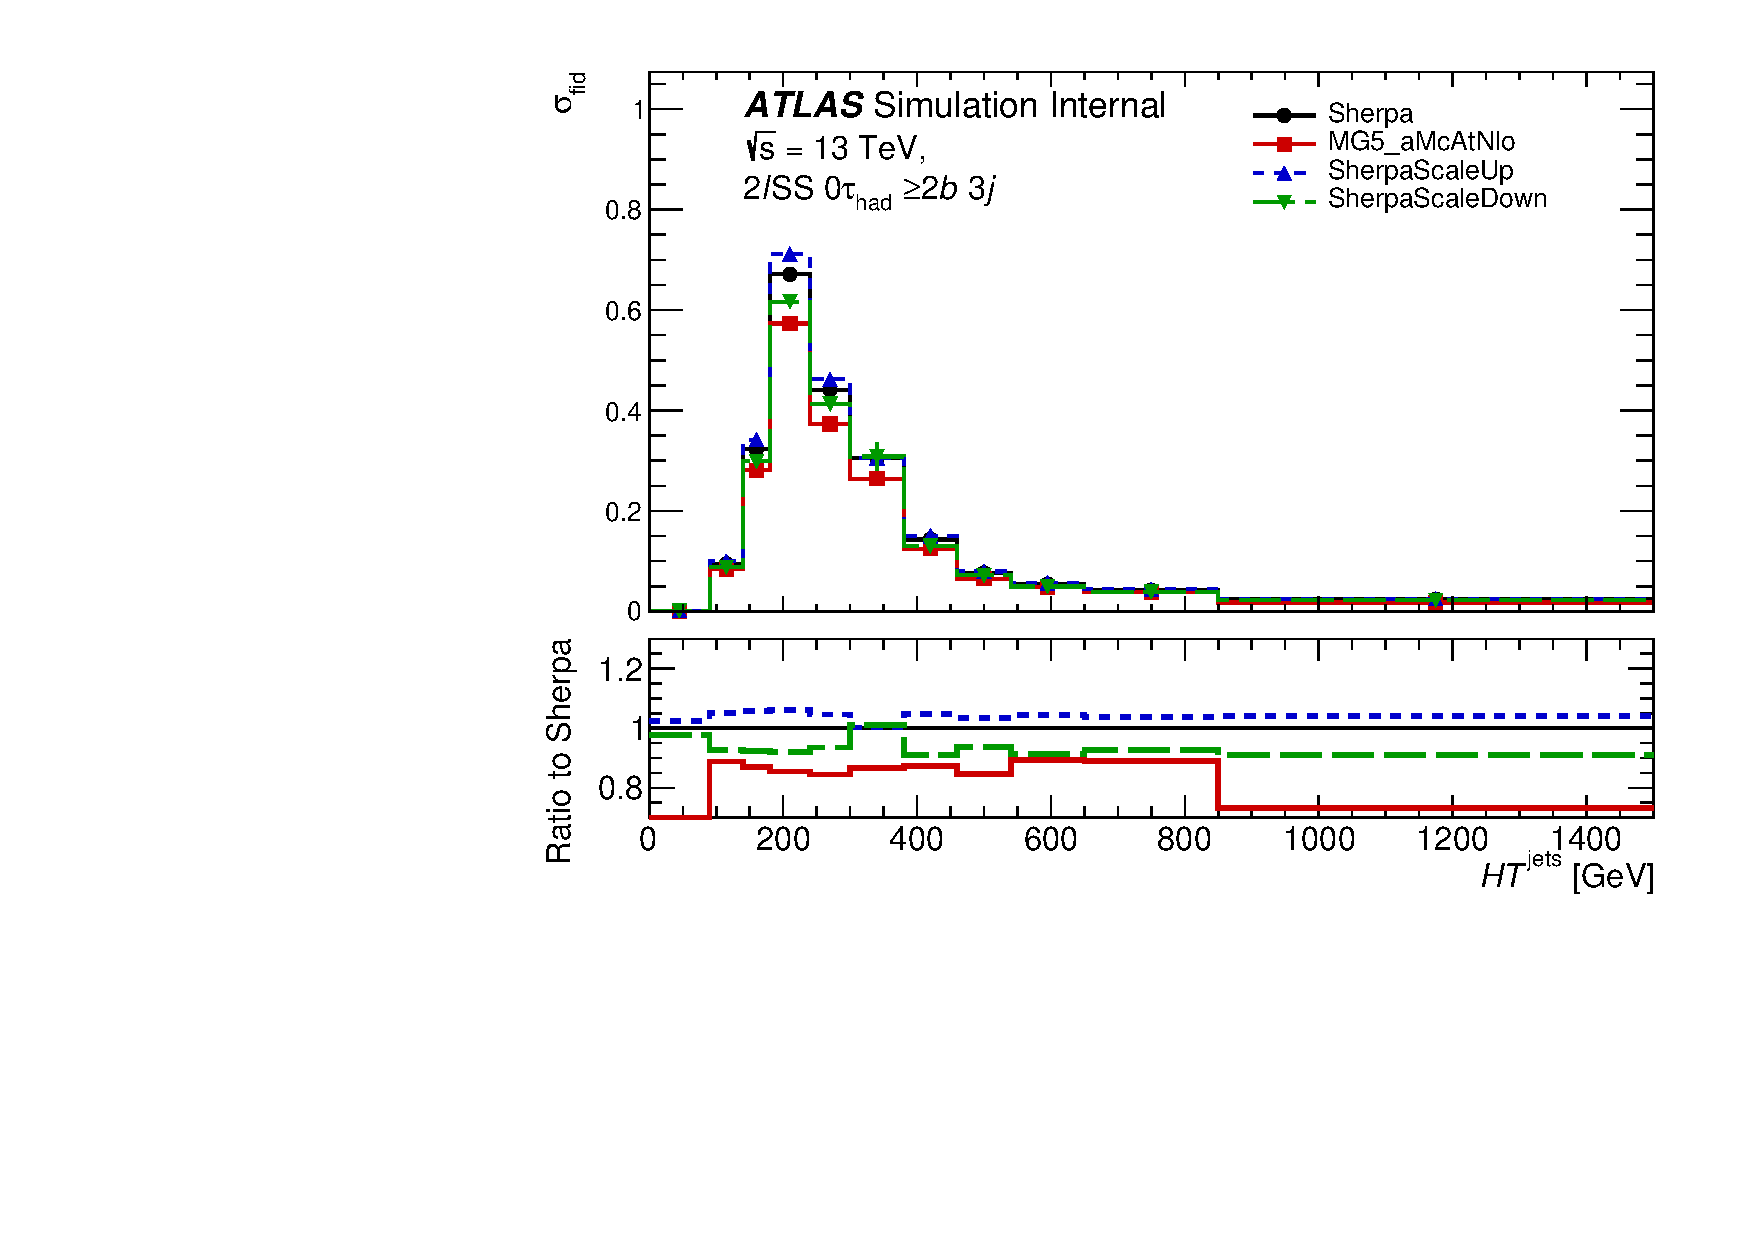
\includegraphics[width=0.45\textwidth]{Plots/ttV/generator/c_Region_3_HT_jets}\\
  \caption{Distribution of the scalar sum of jets transverse momentum, $HT^{\text{jets}}$, for the Region 3 with $N_{b-\mathrm{jets}}$=1 (left) and Region 4 with $N_{b-\mathrm{jets}}\geq$2 (right) selection requiring exactly three jets.  \label{ttV:den_3j12b}}
\end{figure}


\begin{figure}[!htb]
\centering
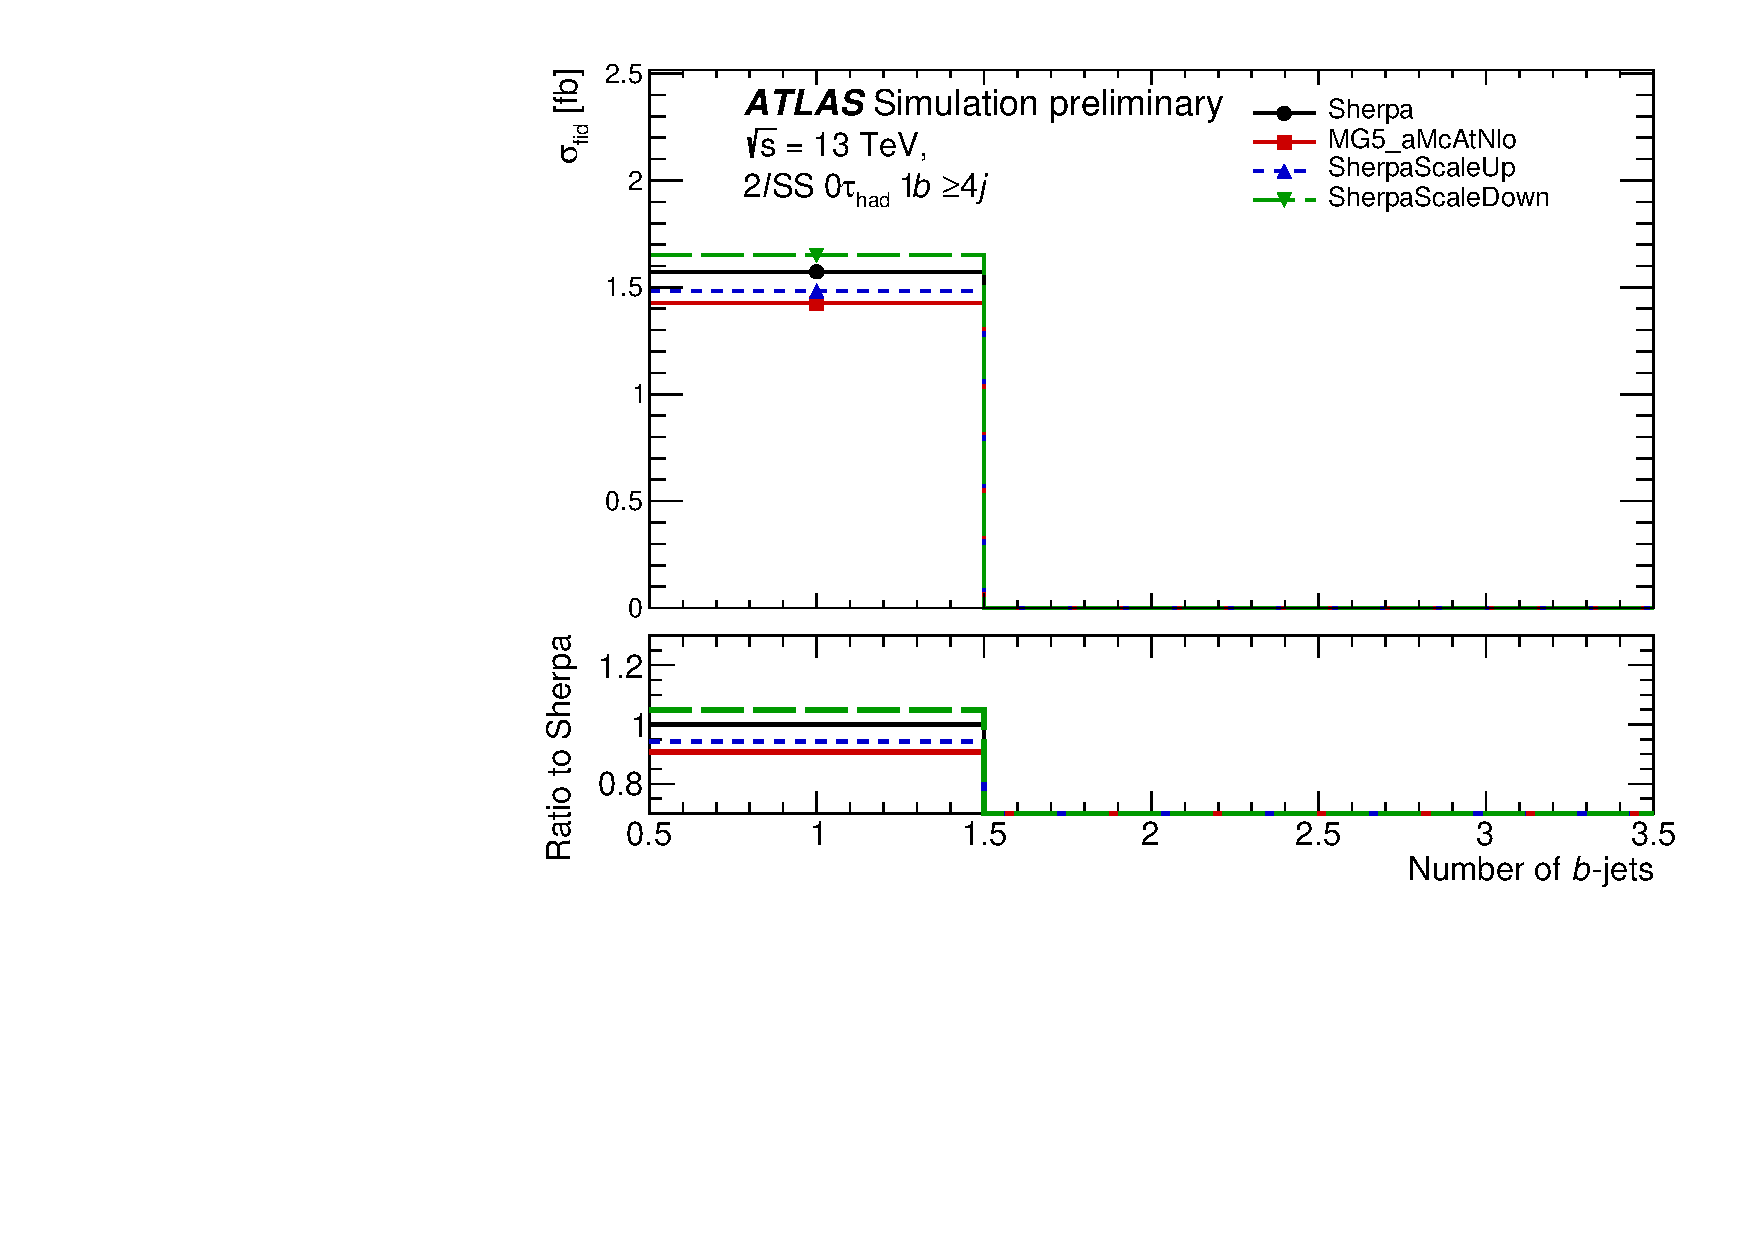
\includegraphics[width=0.45\textwidth]{Plots/ttV/generator/c_Region_0_nBtagJets}
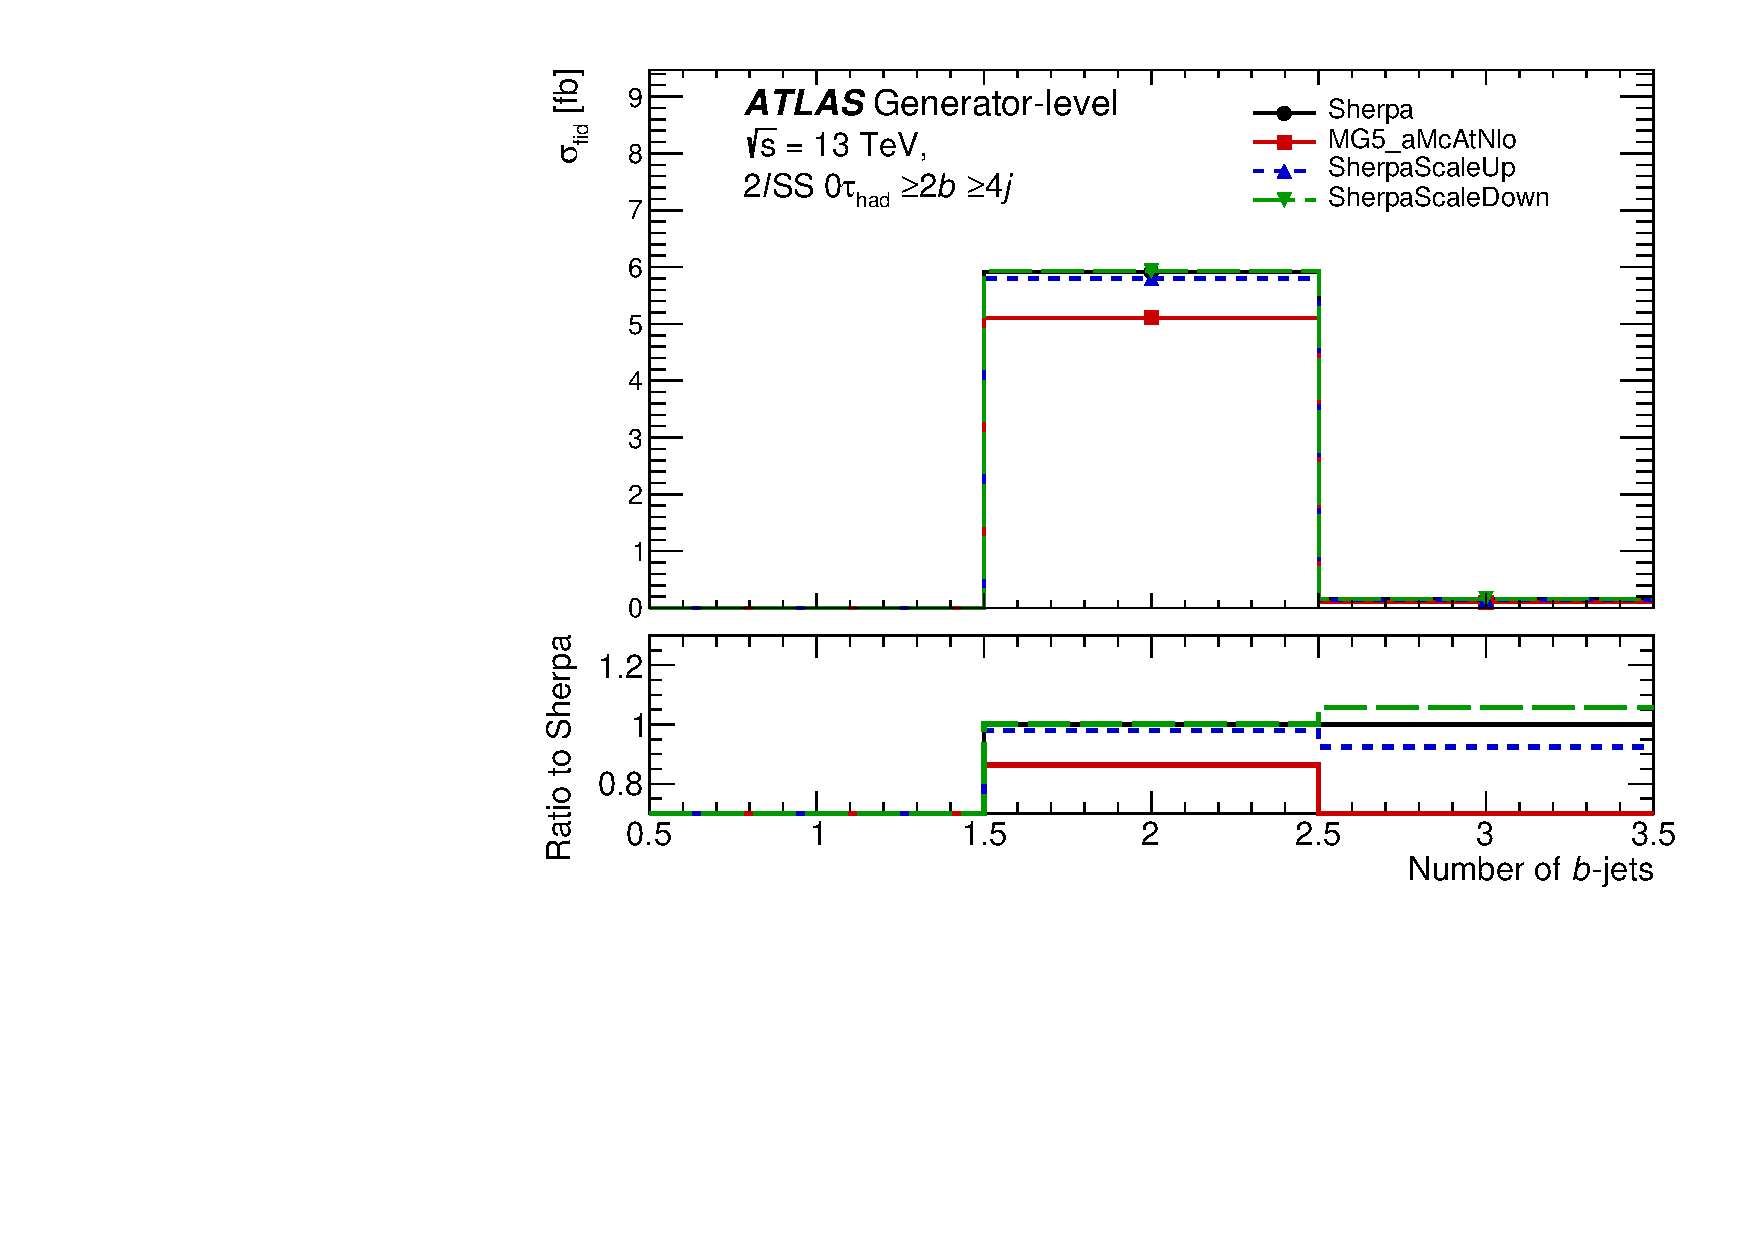
\includegraphics[width=0.45\textwidth]{Plots/ttV/generator/c_Region_1_nBtagJets}\\
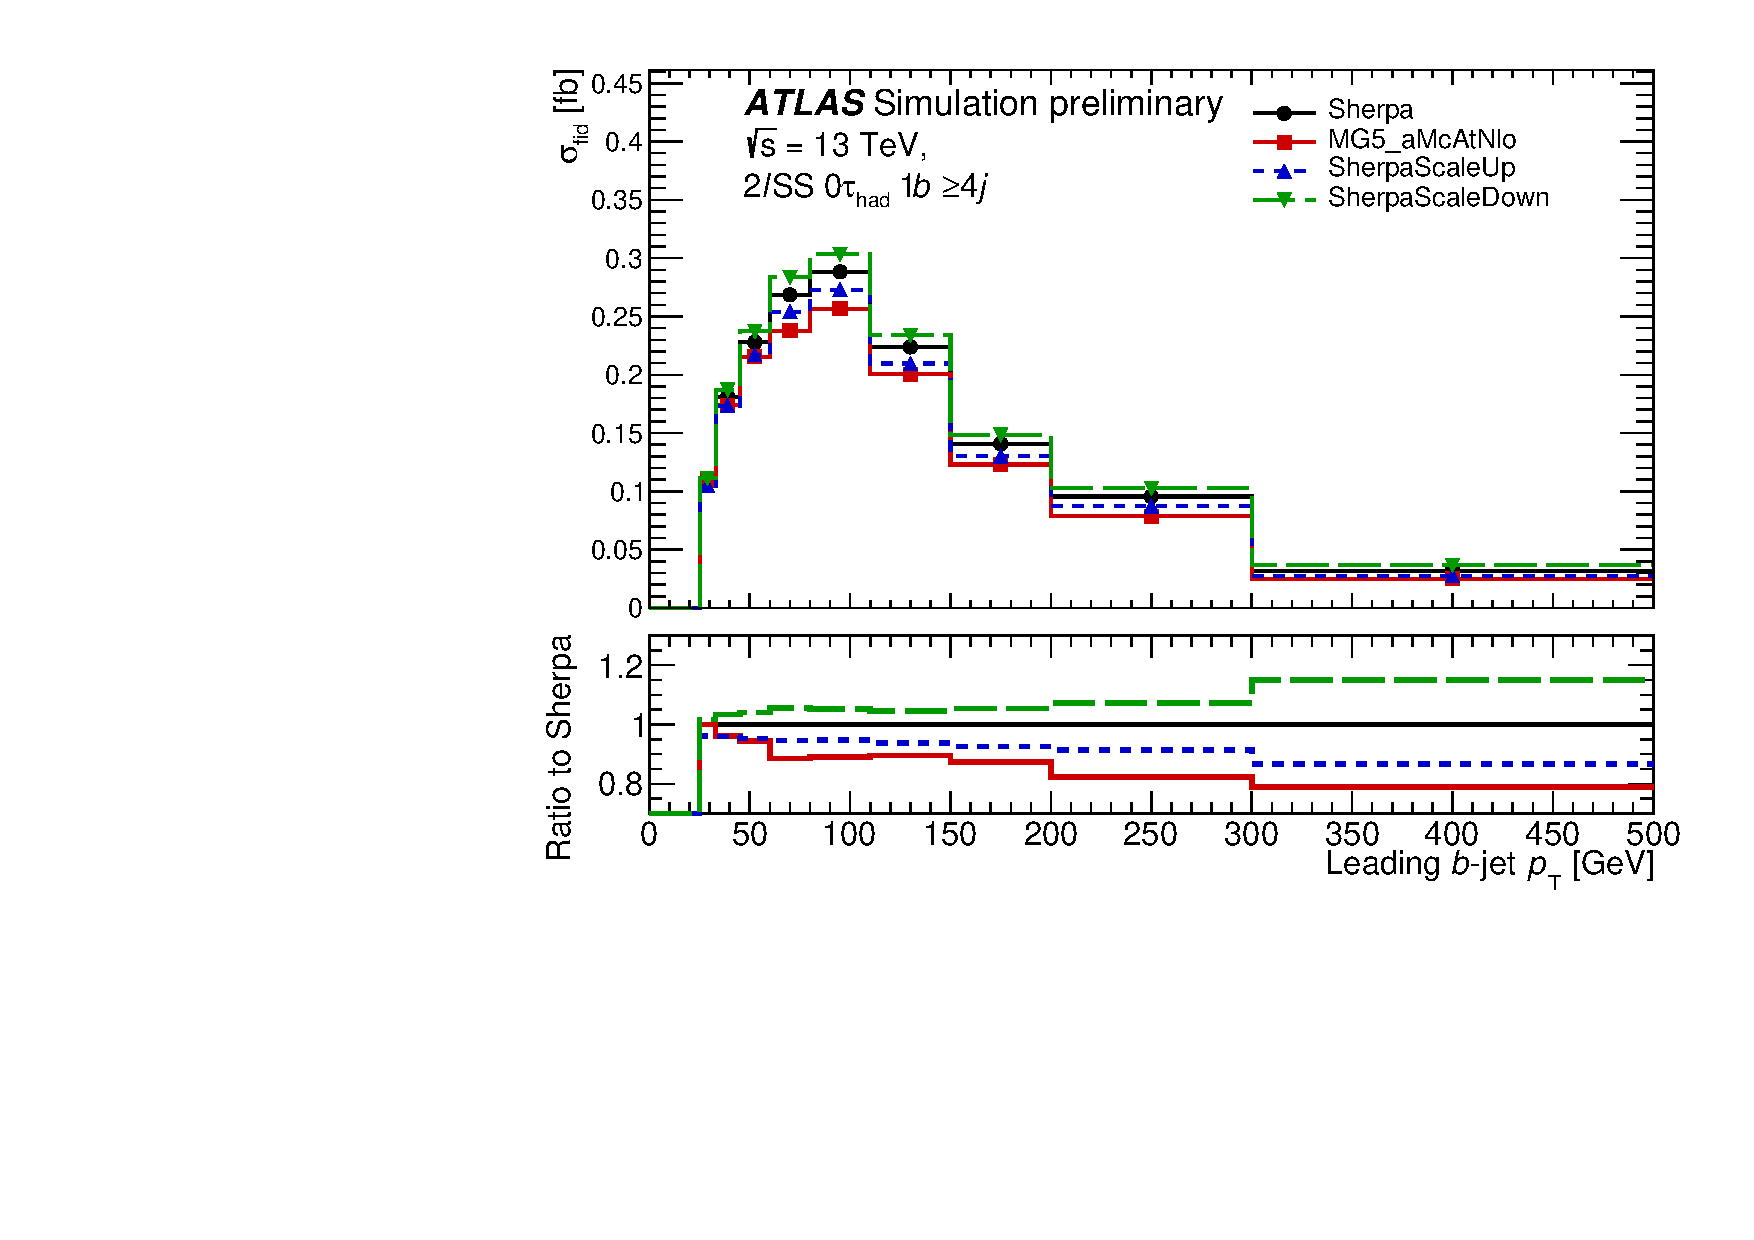
\includegraphics[width=0.45\textwidth]{Plots/ttV/generator/c_Region_0_Bjet_Pt_0}
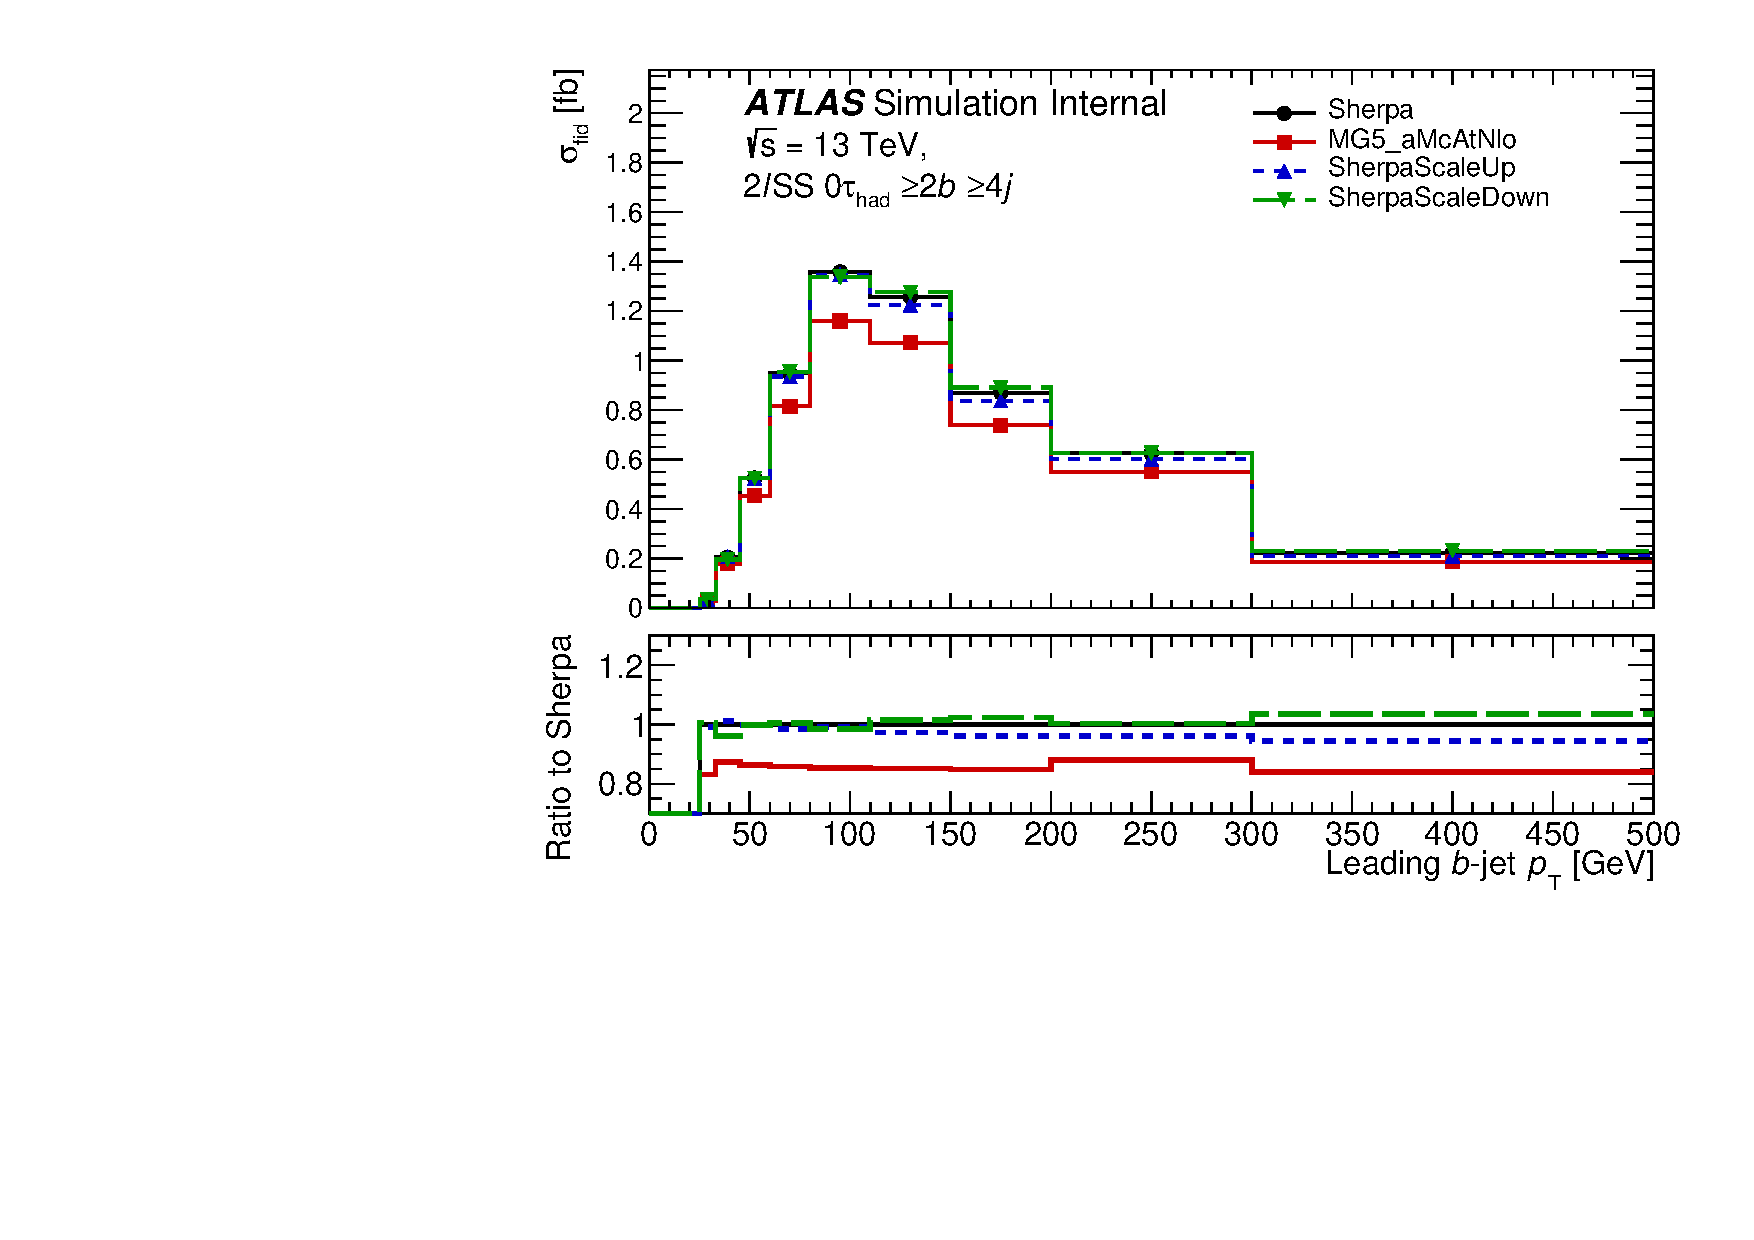
\includegraphics[width=0.45\textwidth]{Plots/ttV/generator/c_Region_1_Bjet_Pt_0}\\
  \caption{Distribution of the $b$-jet multiplicities (top) and the leading $b$-jet transverse momentum (bottom), for the Region 1 with $N_{b-\mathrm{jets}}$=1 (left) and Region 2 with $N_{b-\mathrm{jets}}\geq$2 (right) selection requiring four and more jets.  \label{ttV:den_4jbinfo}}
\end{figure}



\begin{figure}[!htb]
\centering
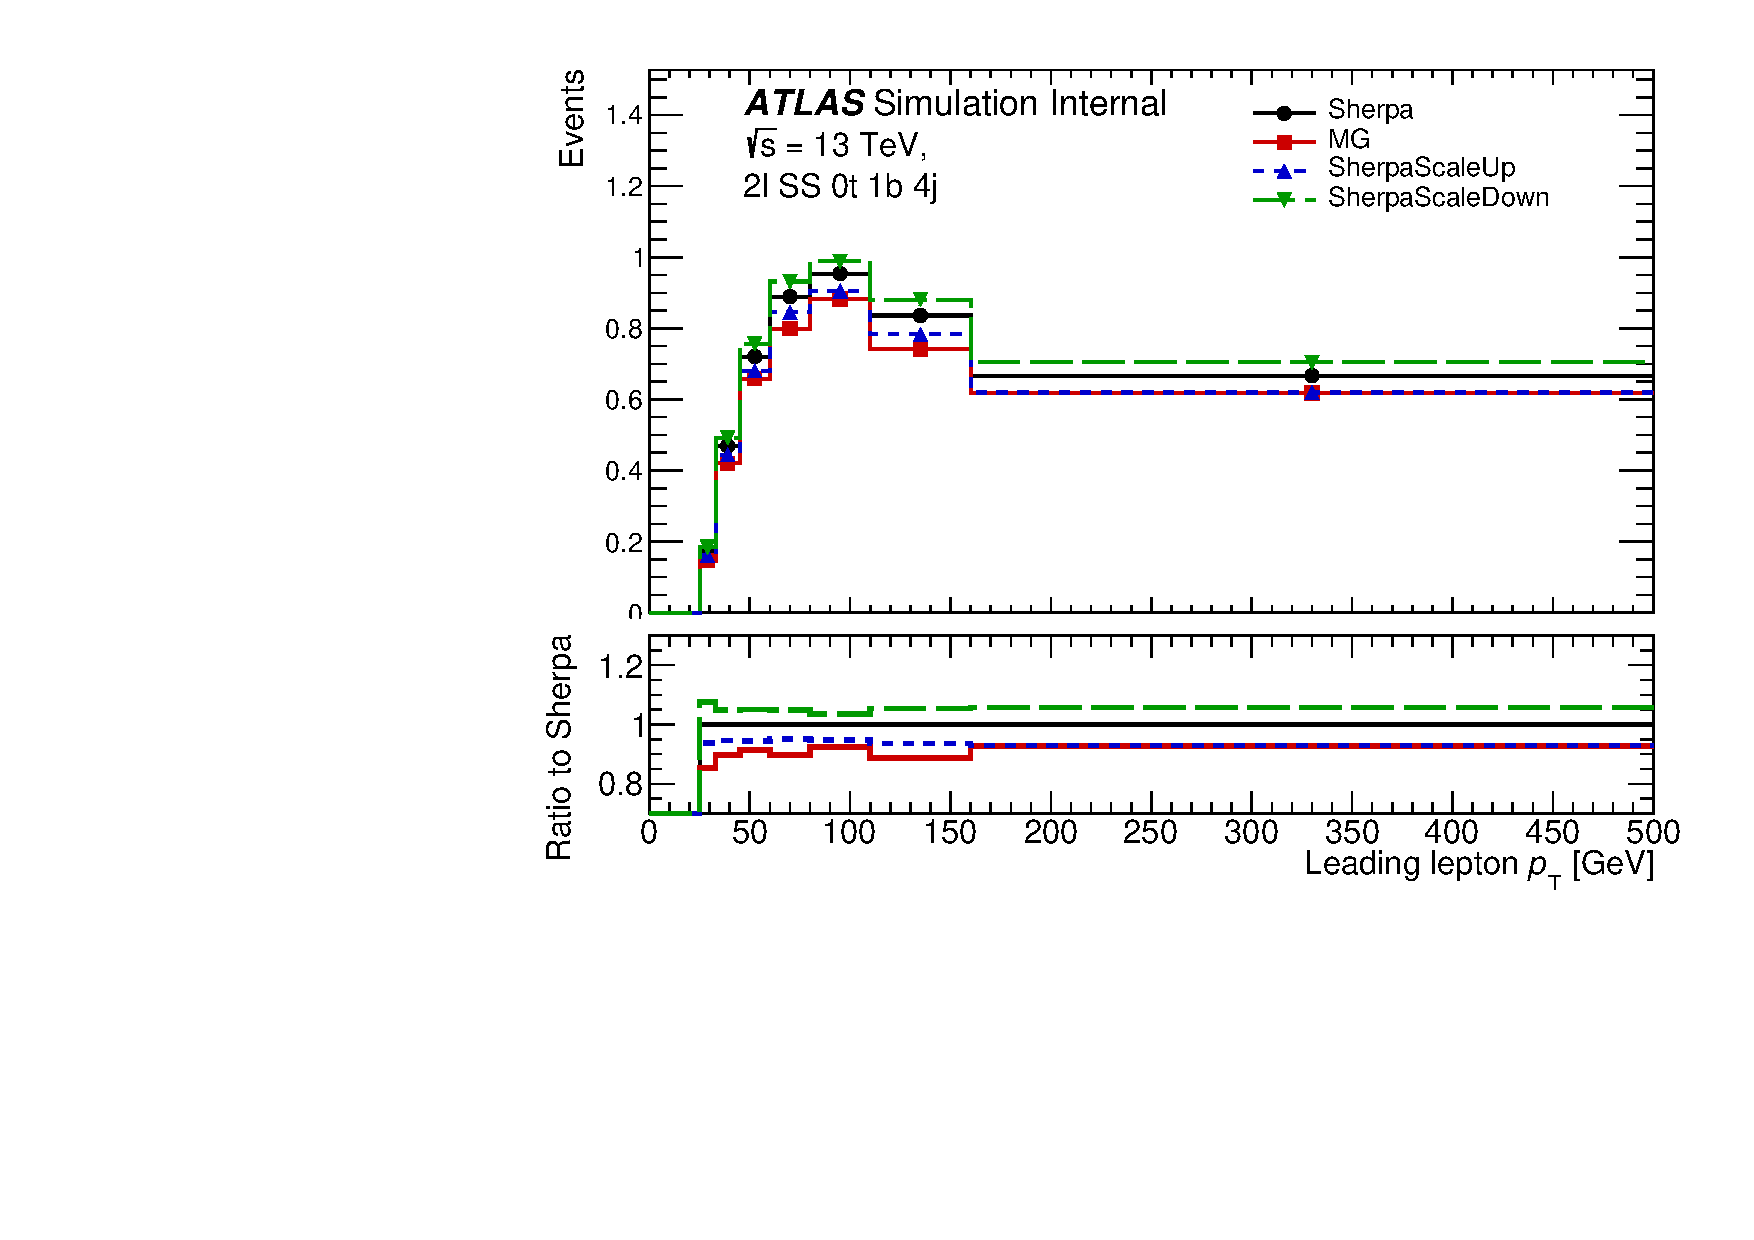
\includegraphics[width=0.45\textwidth]{Plots/ttV/generator/c_Region_0_lep_Pt_0}
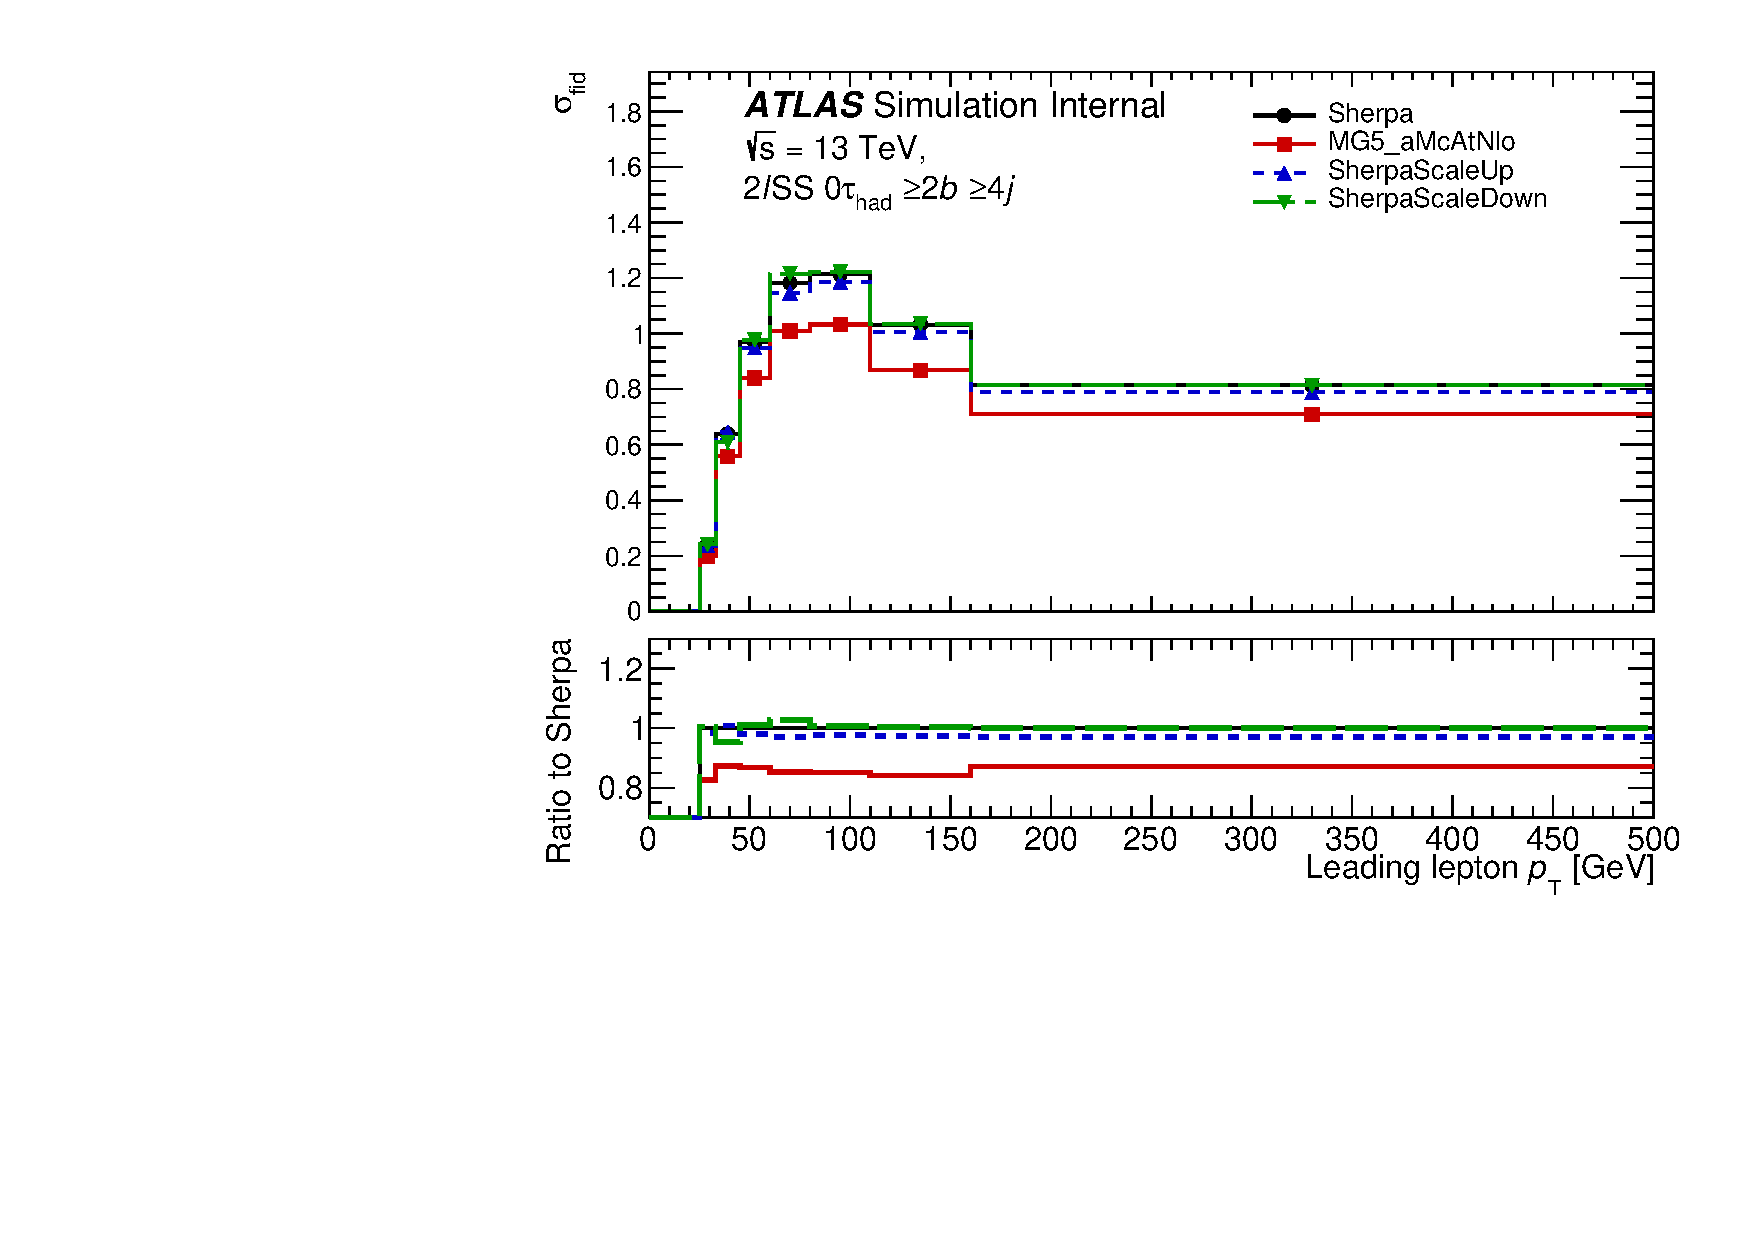
\includegraphics[width=0.45\textwidth]{Plots/ttV/generator/c_Region_1_lep_Pt_0}\\
%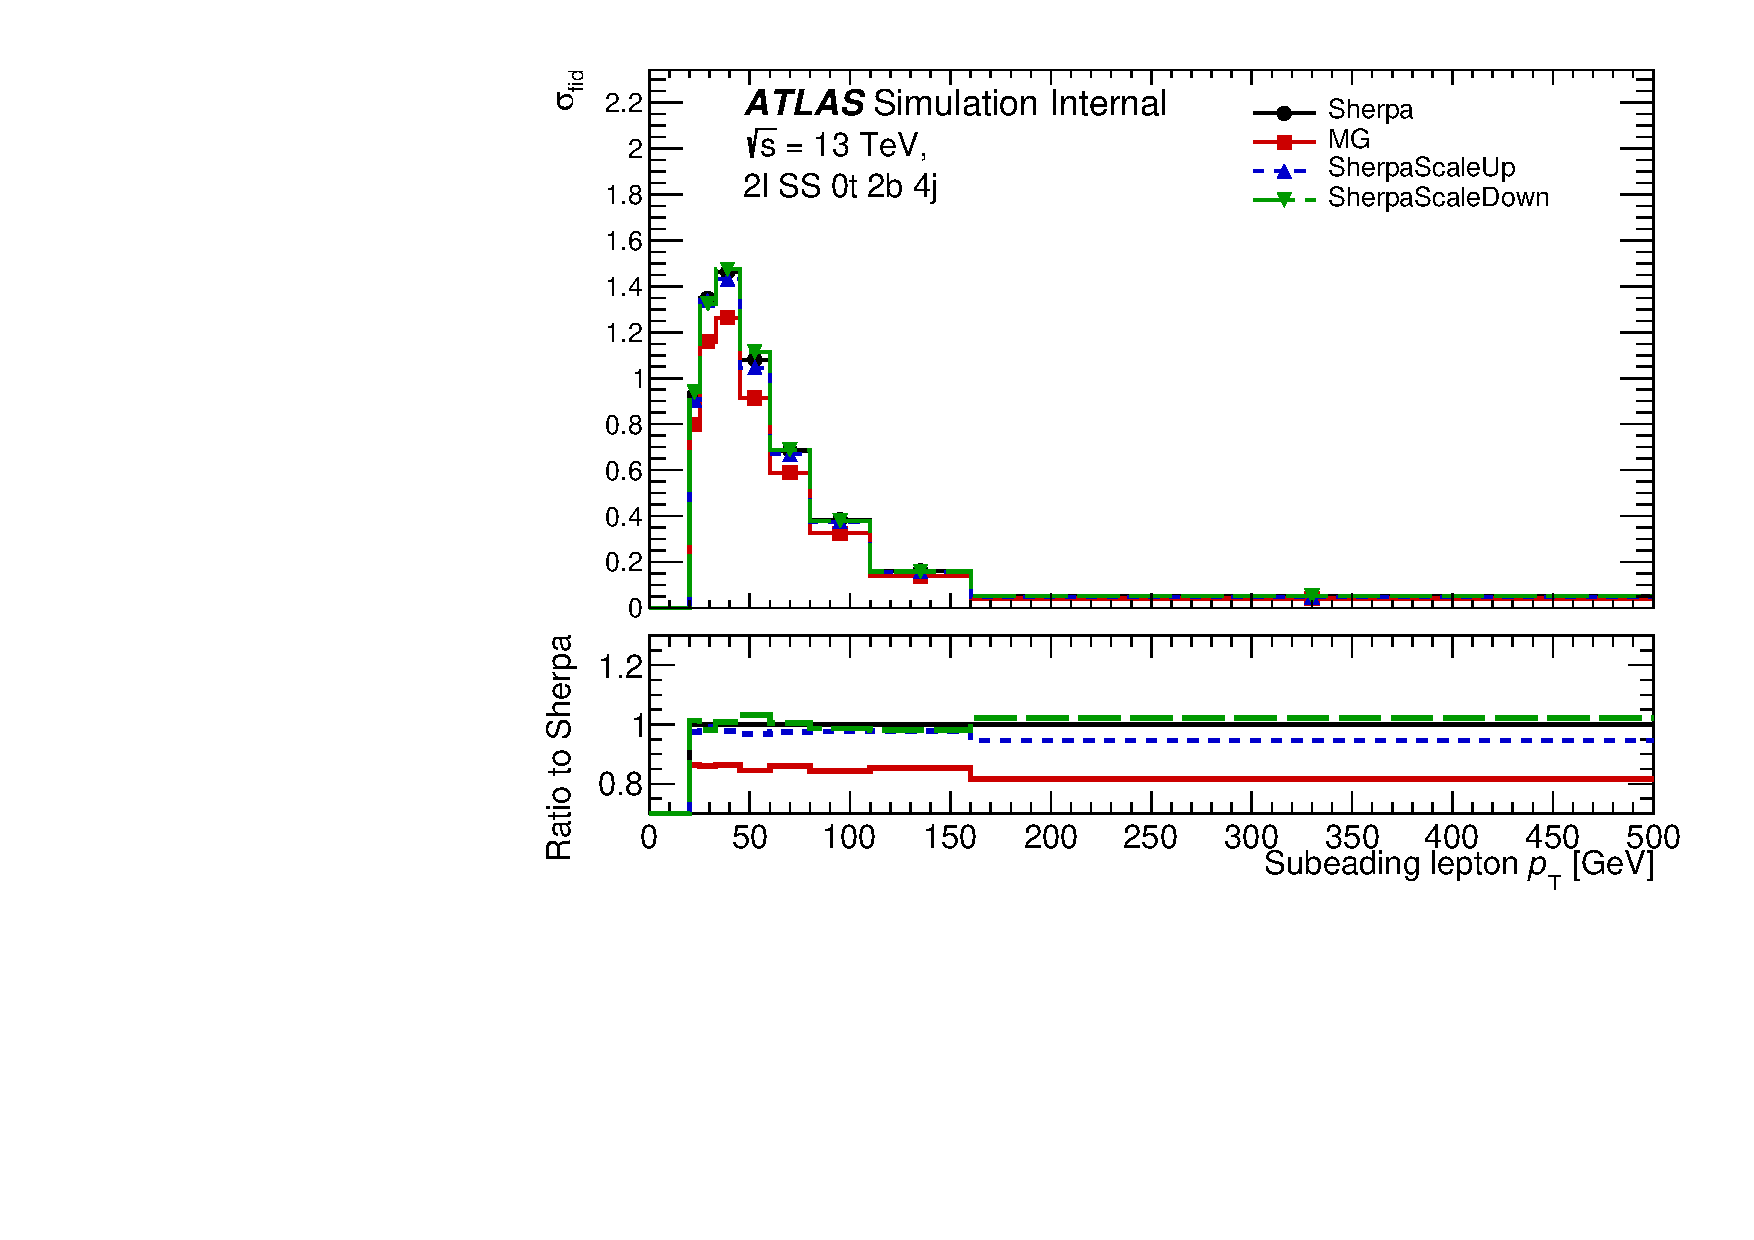
\includegraphics[width=0.45\textwidth]{Plots/ttV/generator/c_Region_1_lep_Pt_1}
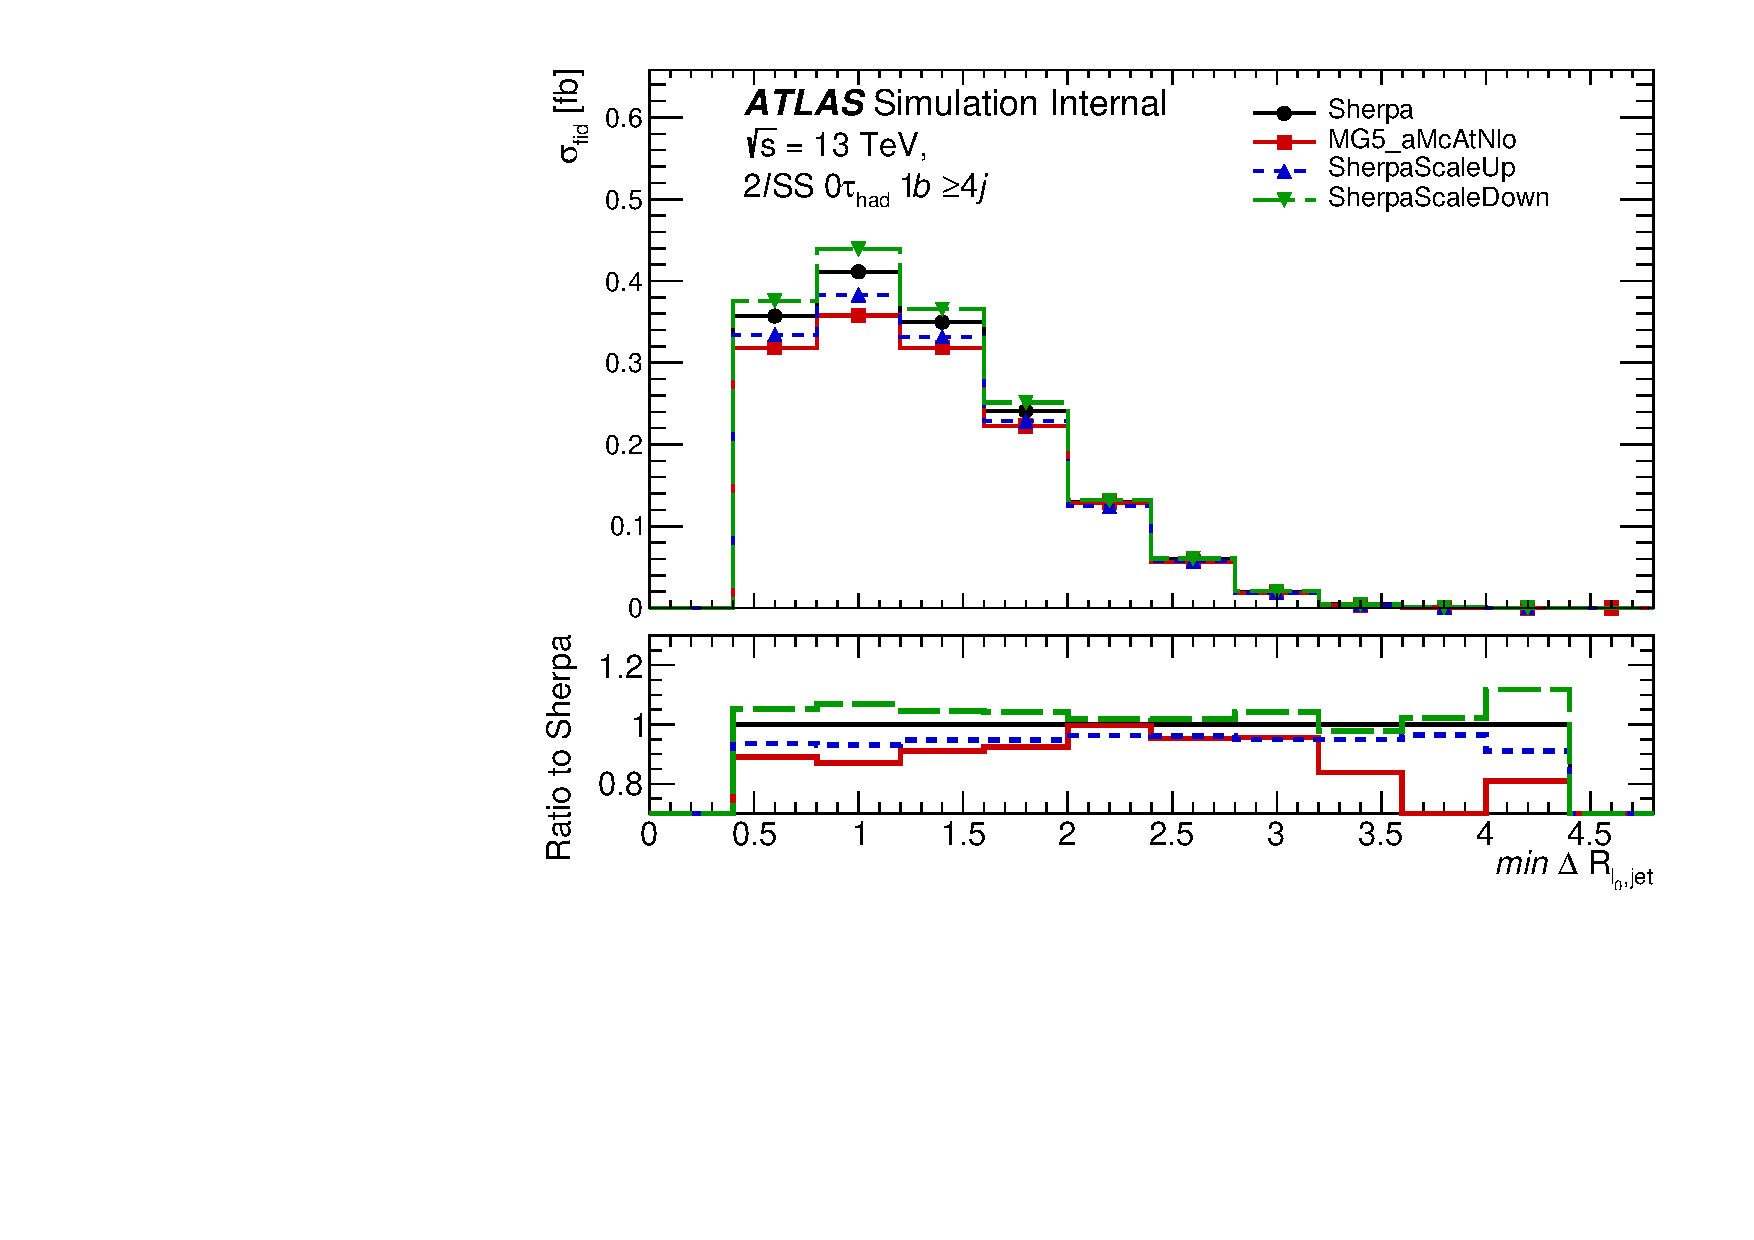
\includegraphics[width=0.45\textwidth]{Plots/ttV/generator/c_Region_0_min_DRl0j}
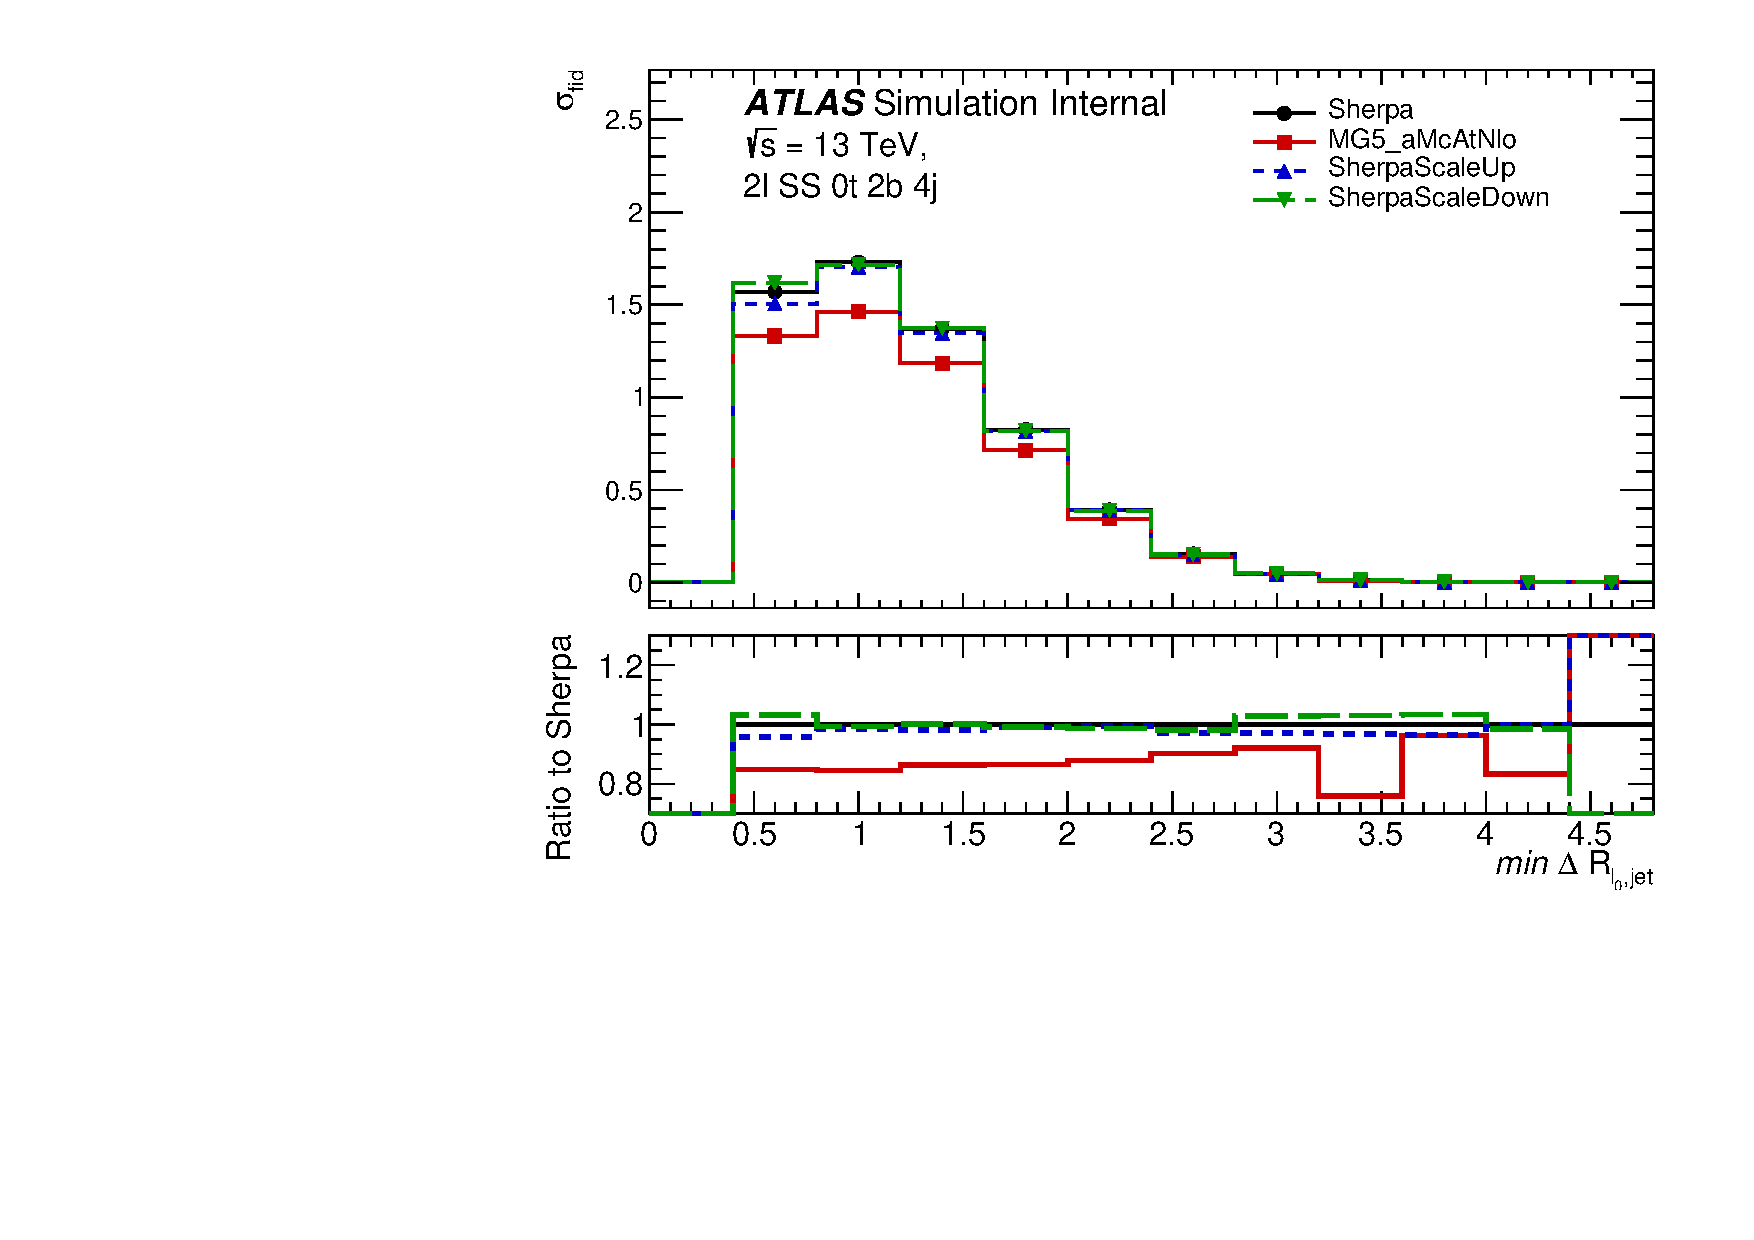
\includegraphics[width=0.45\textwidth]{Plots/ttV/generator/c_Region_1_min_DRl0j}\\
  \caption{Distribution of the leading lepton transverse momentum (top) and the minimum angular separation between the leading lepton and the nearest jet (bottom), for the Region 1 with $N_{b-\mathrm{jets}}$=1 (left) and Region 2 with $N_{b-\mathrm{jets}}\geq$2 (right) selection requiring four and more jets. 
  \label{ttV:den_lep_kin}}
\end{figure}

\begin{figure}[!htb]
\centering
	% \hspace{25mm} $DRl_0l_1$  \hspace{20mm} $max|\eta^{\ell\ell}|$\\
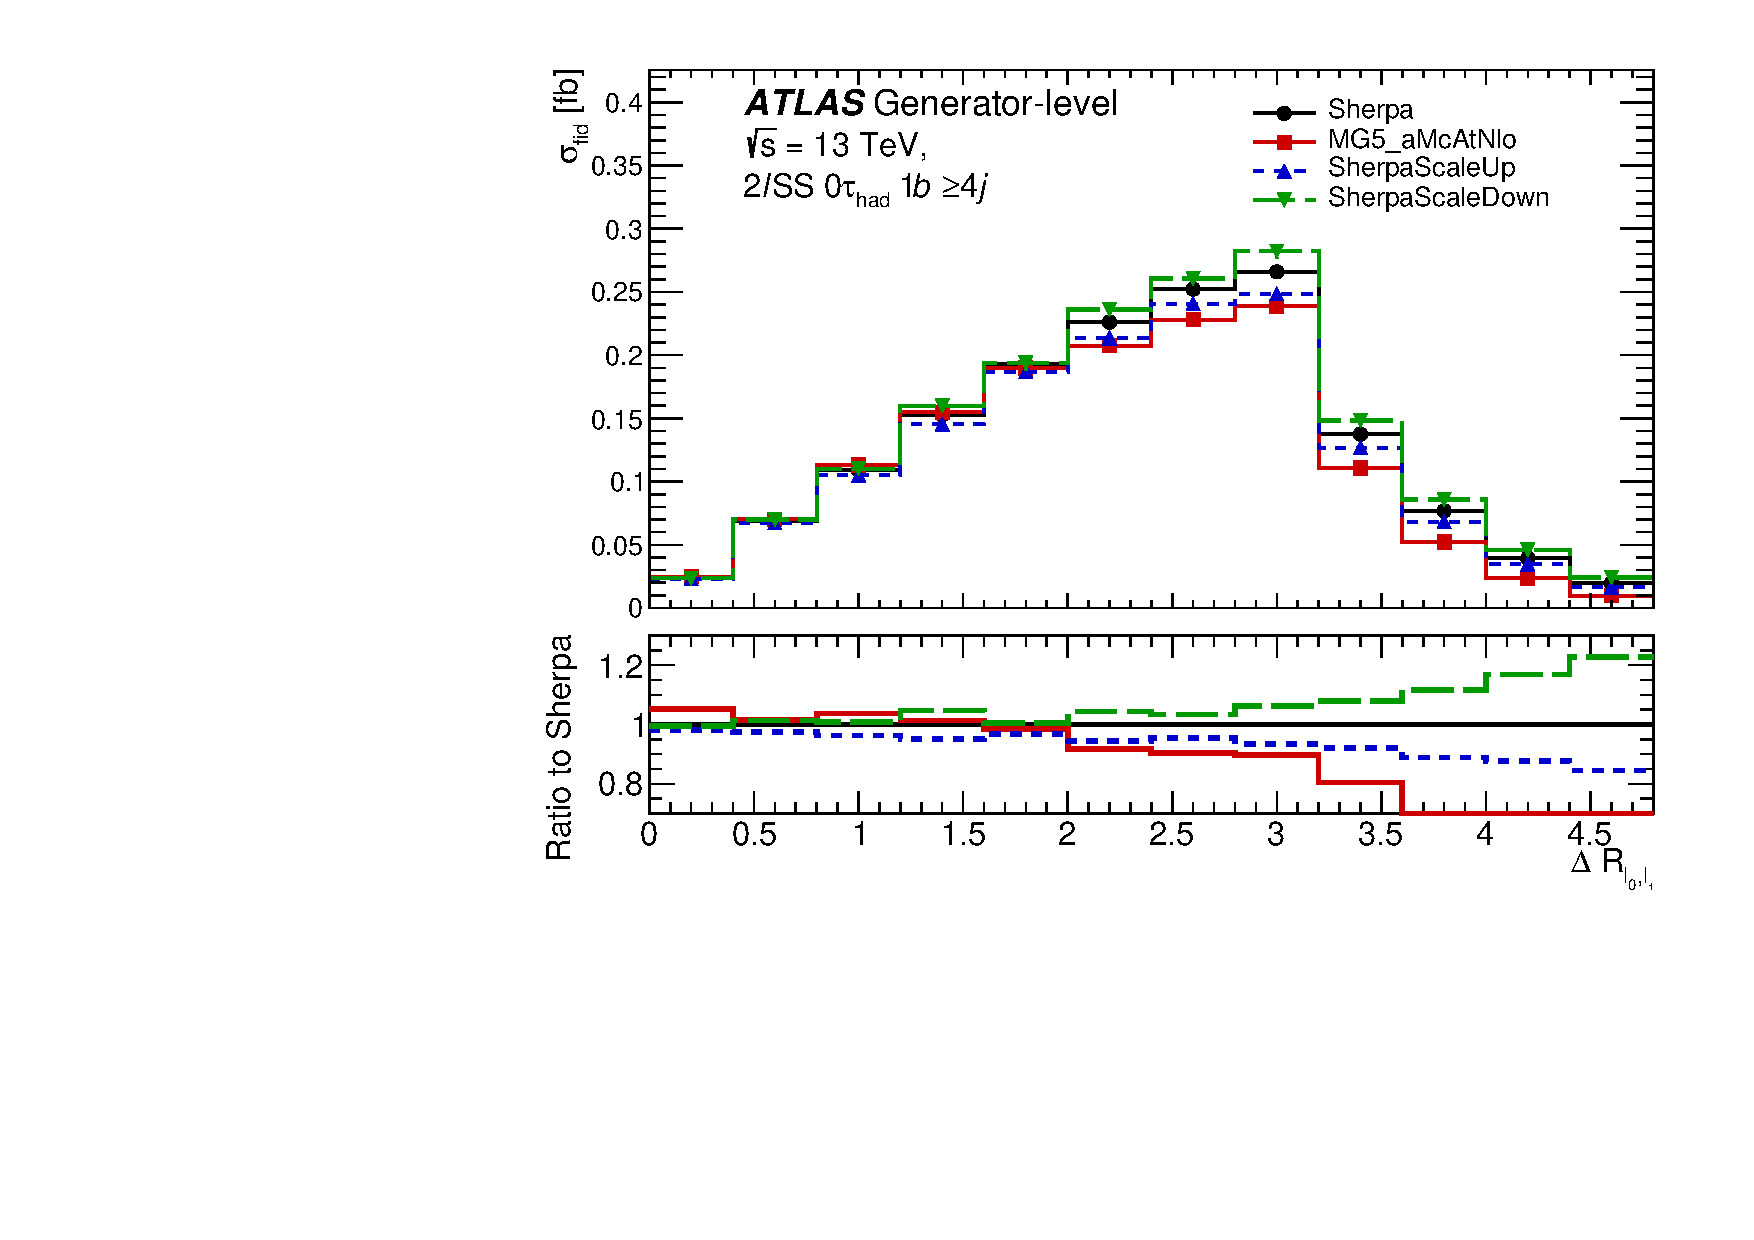
\includegraphics[width=0.45\textwidth]{Plots/ttV/generator/c_Region_0_DRll01}
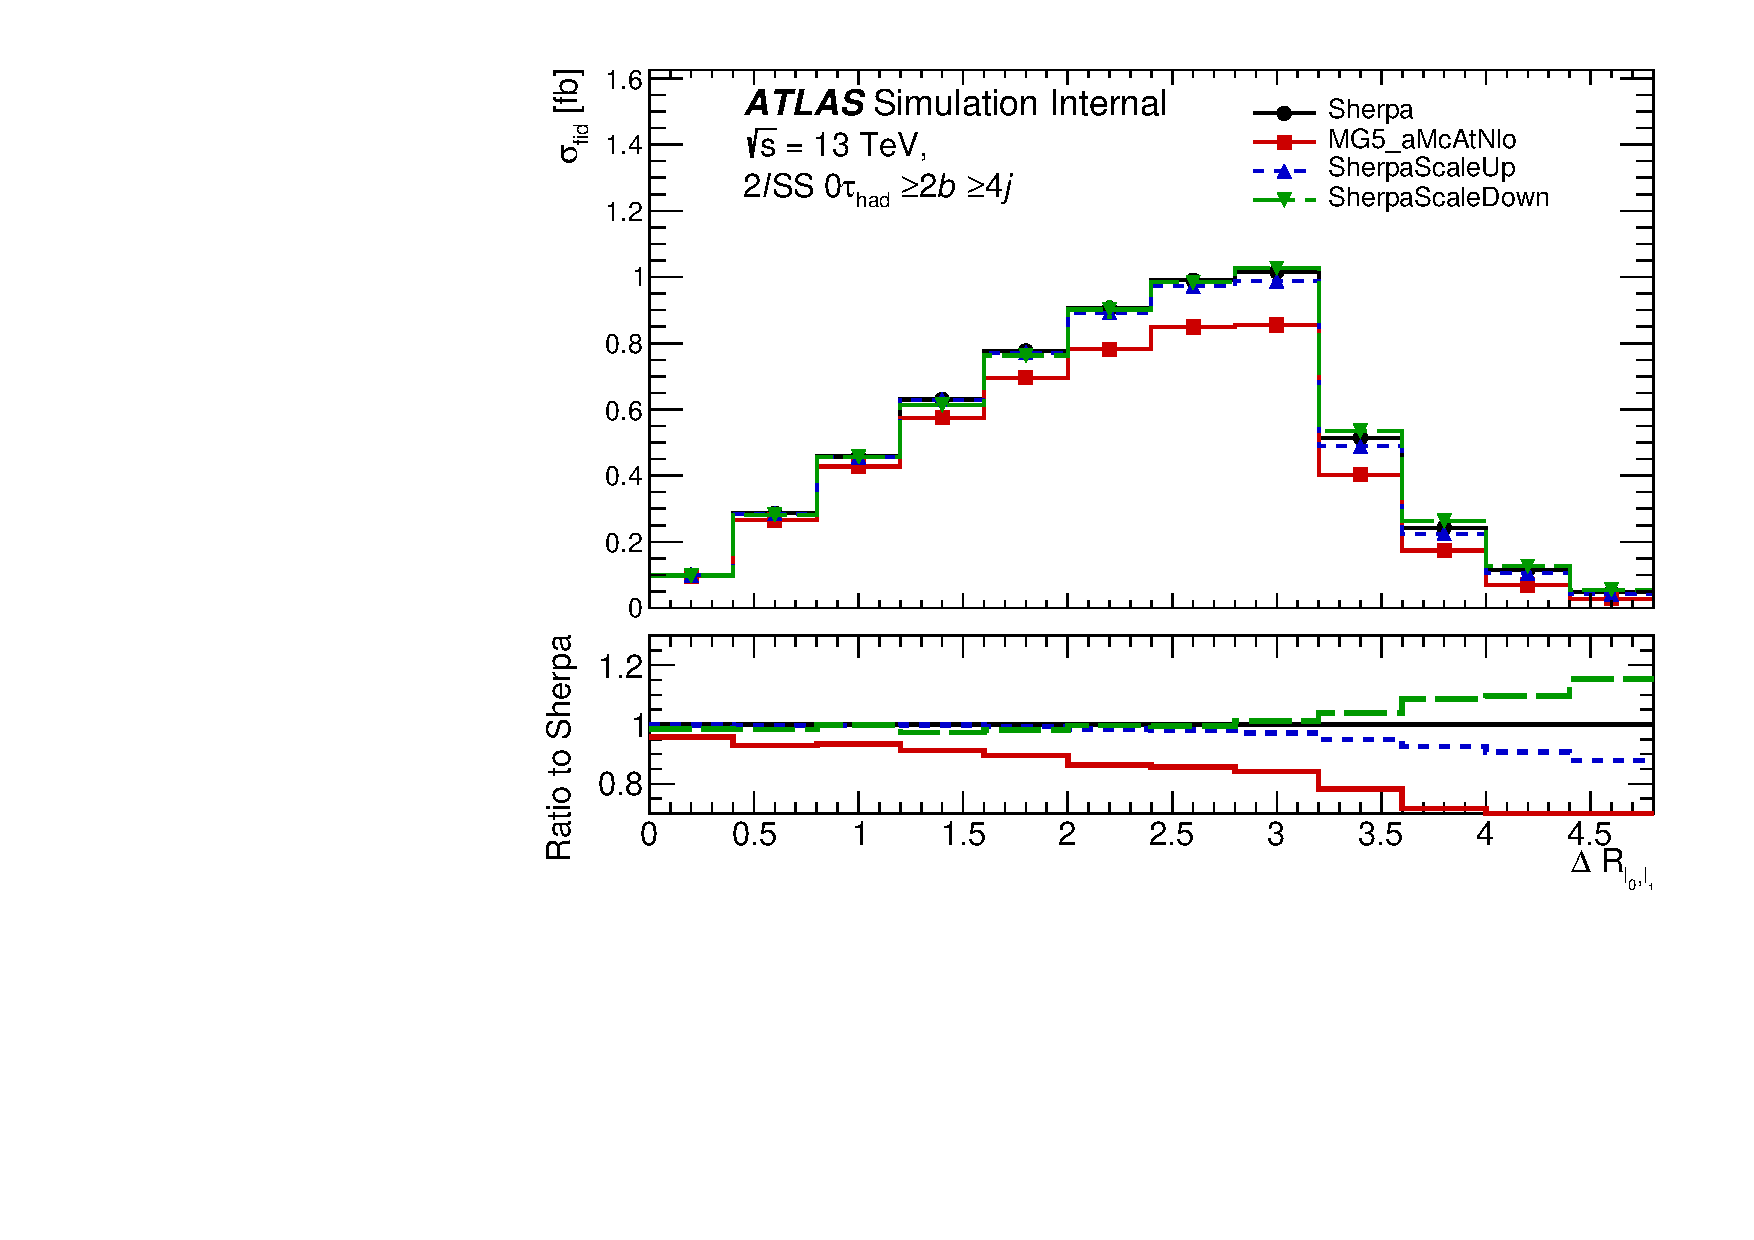
\includegraphics[width=0.45\textwidth]{Plots/ttV/generator/c_Region_1_DRll01}\\
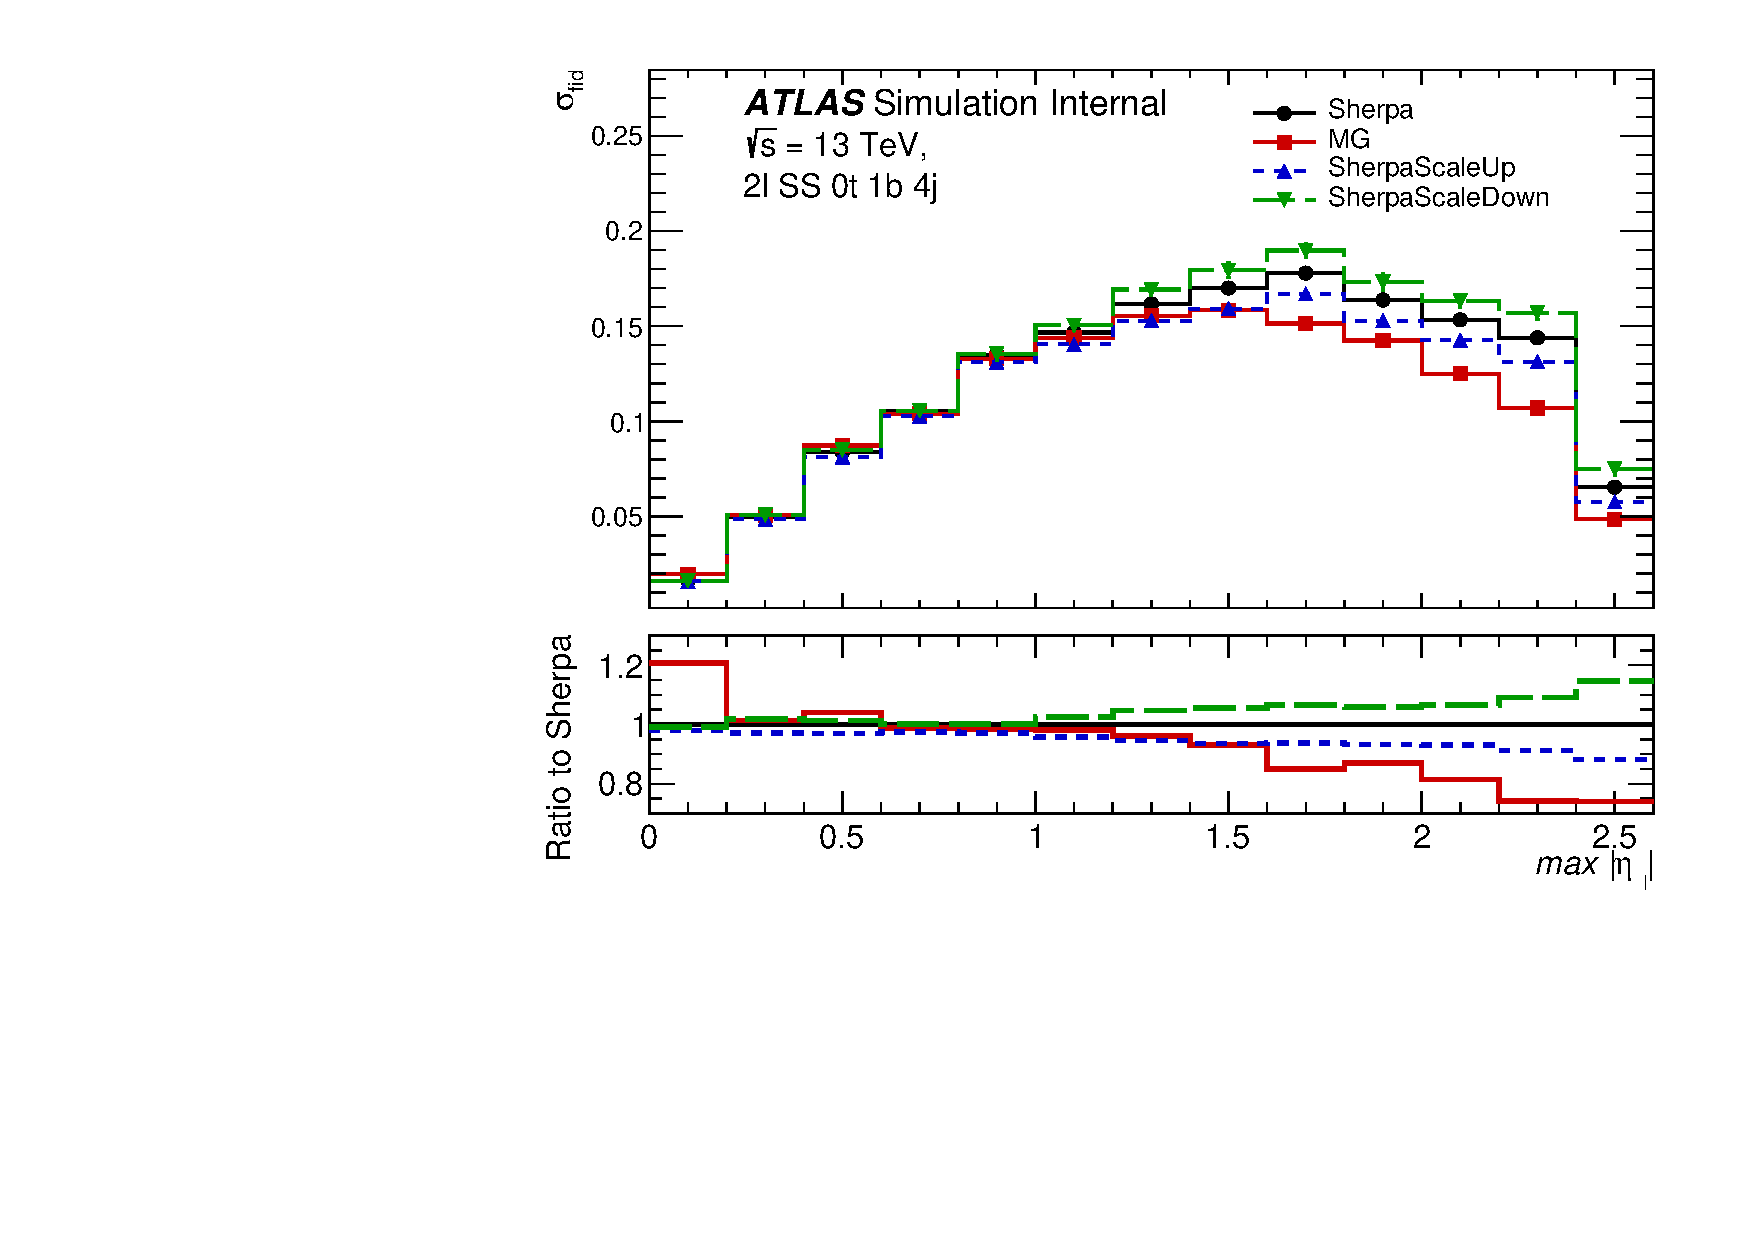
\includegraphics[width=0.45\textwidth]{Plots/ttV/generator/c_Region_0_maxEta_ll} 
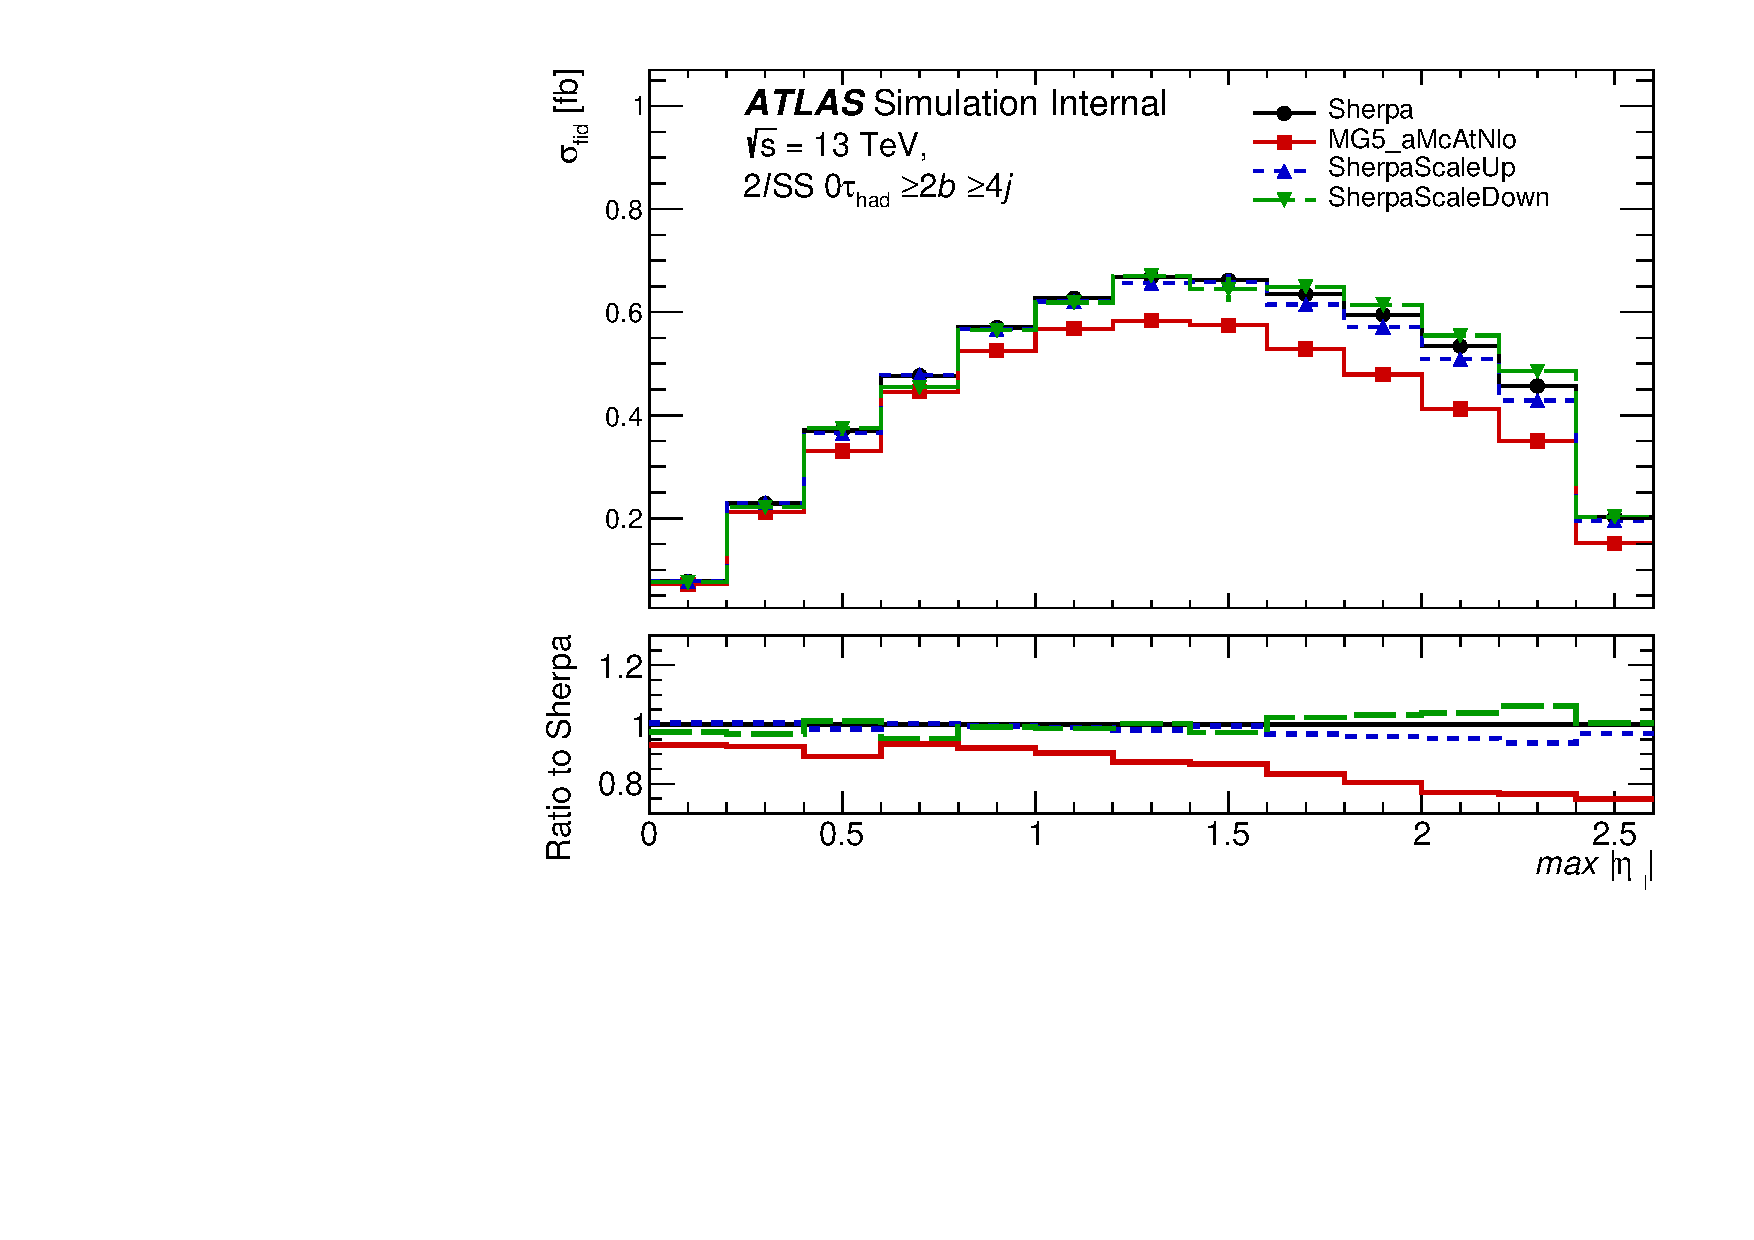
\includegraphics[width=0.45\textwidth]{Plots/ttV/generator/c_Region_1_maxEta_ll}\\
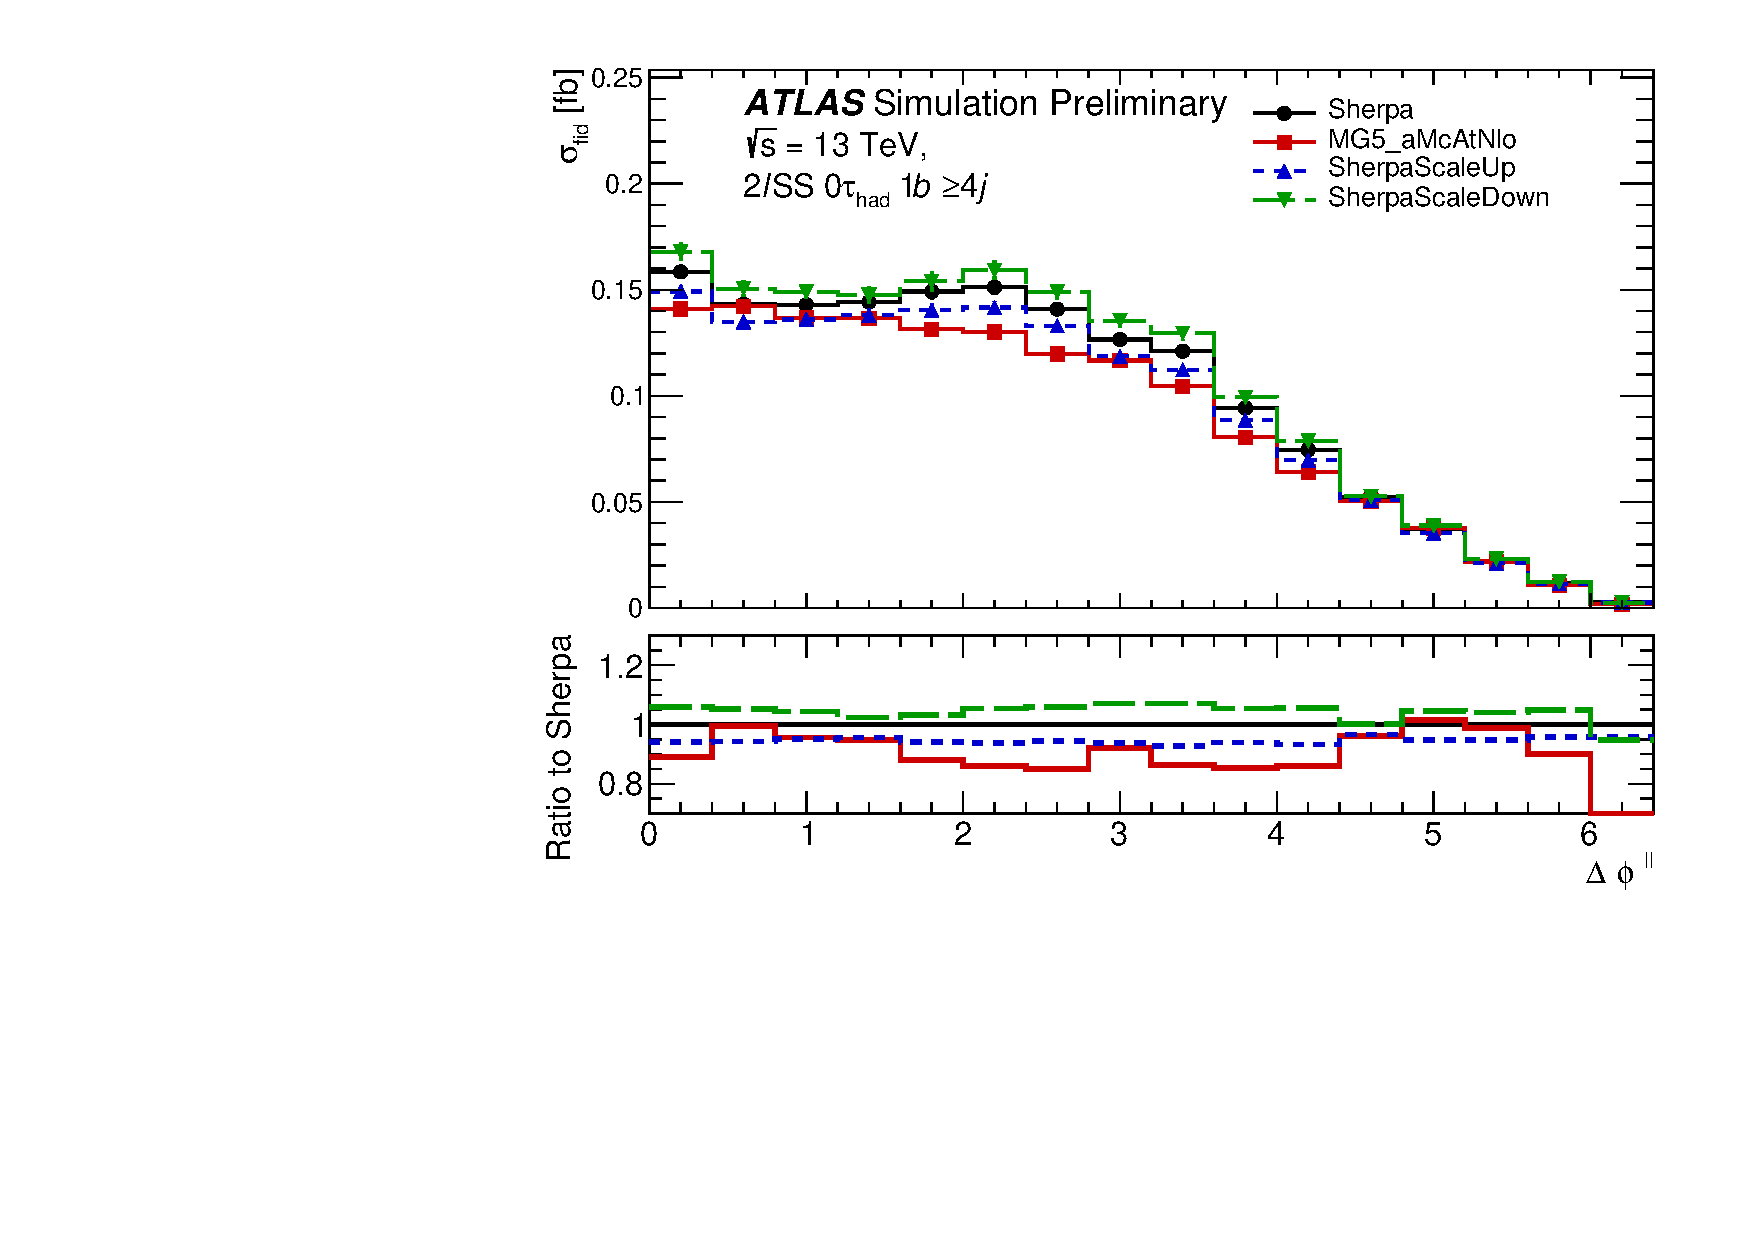
\includegraphics[width=0.45\textwidth]{Plots/ttV/generator/c_Region_0_lep_dPhi} 
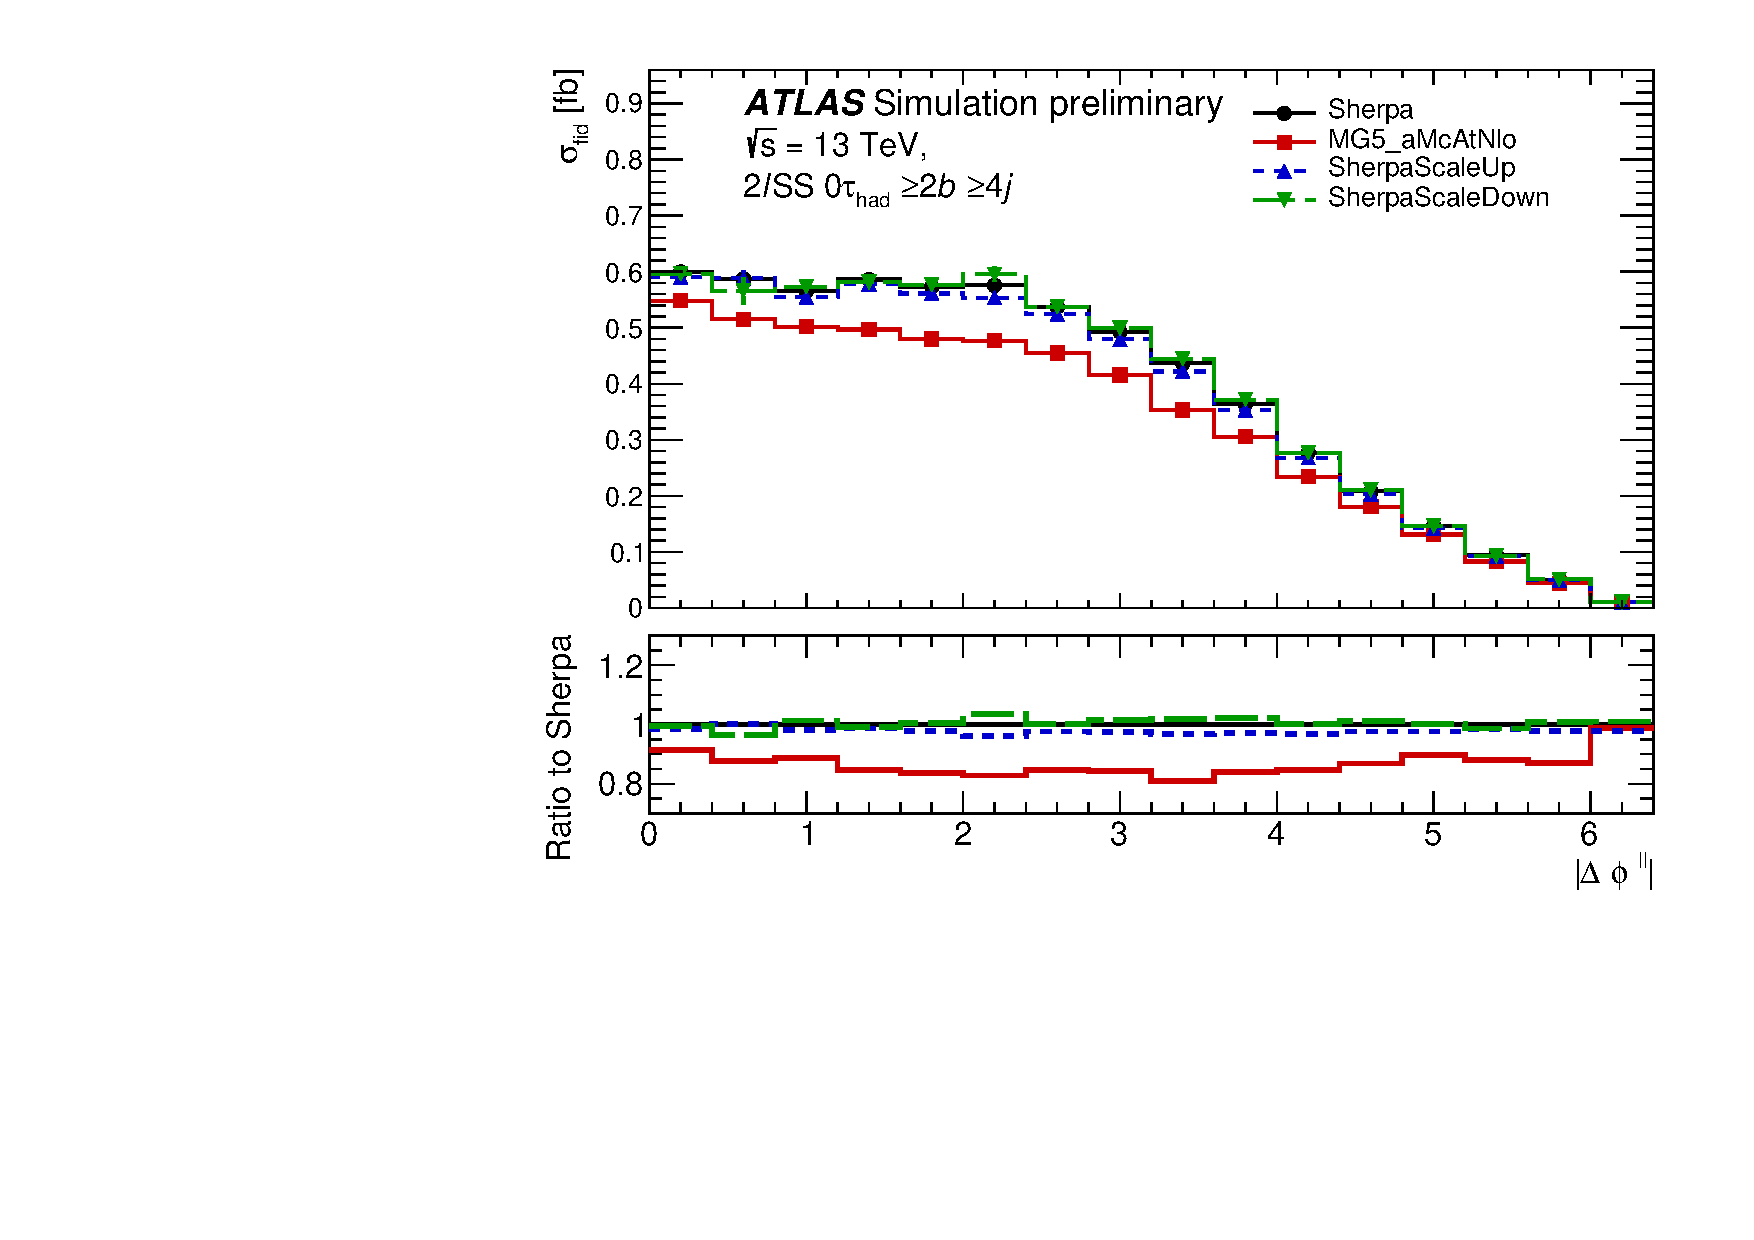
\includegraphics[width=0.45\textwidth]{Plots/ttV/generator/c_Region_1_lep_dPhi} 
  \caption{Distribution of the angular distance between the two leptons (top), maximum between lepton $|\eta_{\ell 0}|$ and $|\eta_{\ell 1}|$ (centre), azimuthal separation between the leptons $\Delta \phi _{\ell \ell }$ (bottom) , for the Region 1 with $N_{b-\mathrm{jets}}$=1 (left) and Region 2 with $N_{b-\mathrm{jets}}\geq$2 (right) selection requiring four and more jets. 
   \label{ttV:den_ll_kin}}
\end{figure}
% 



\begin{figure}[!htb]
\centering
	% \hspace{25mm} $DRl_0l_1$  \hspace{20mm} $max|\eta^{\ell\ell}|$\\
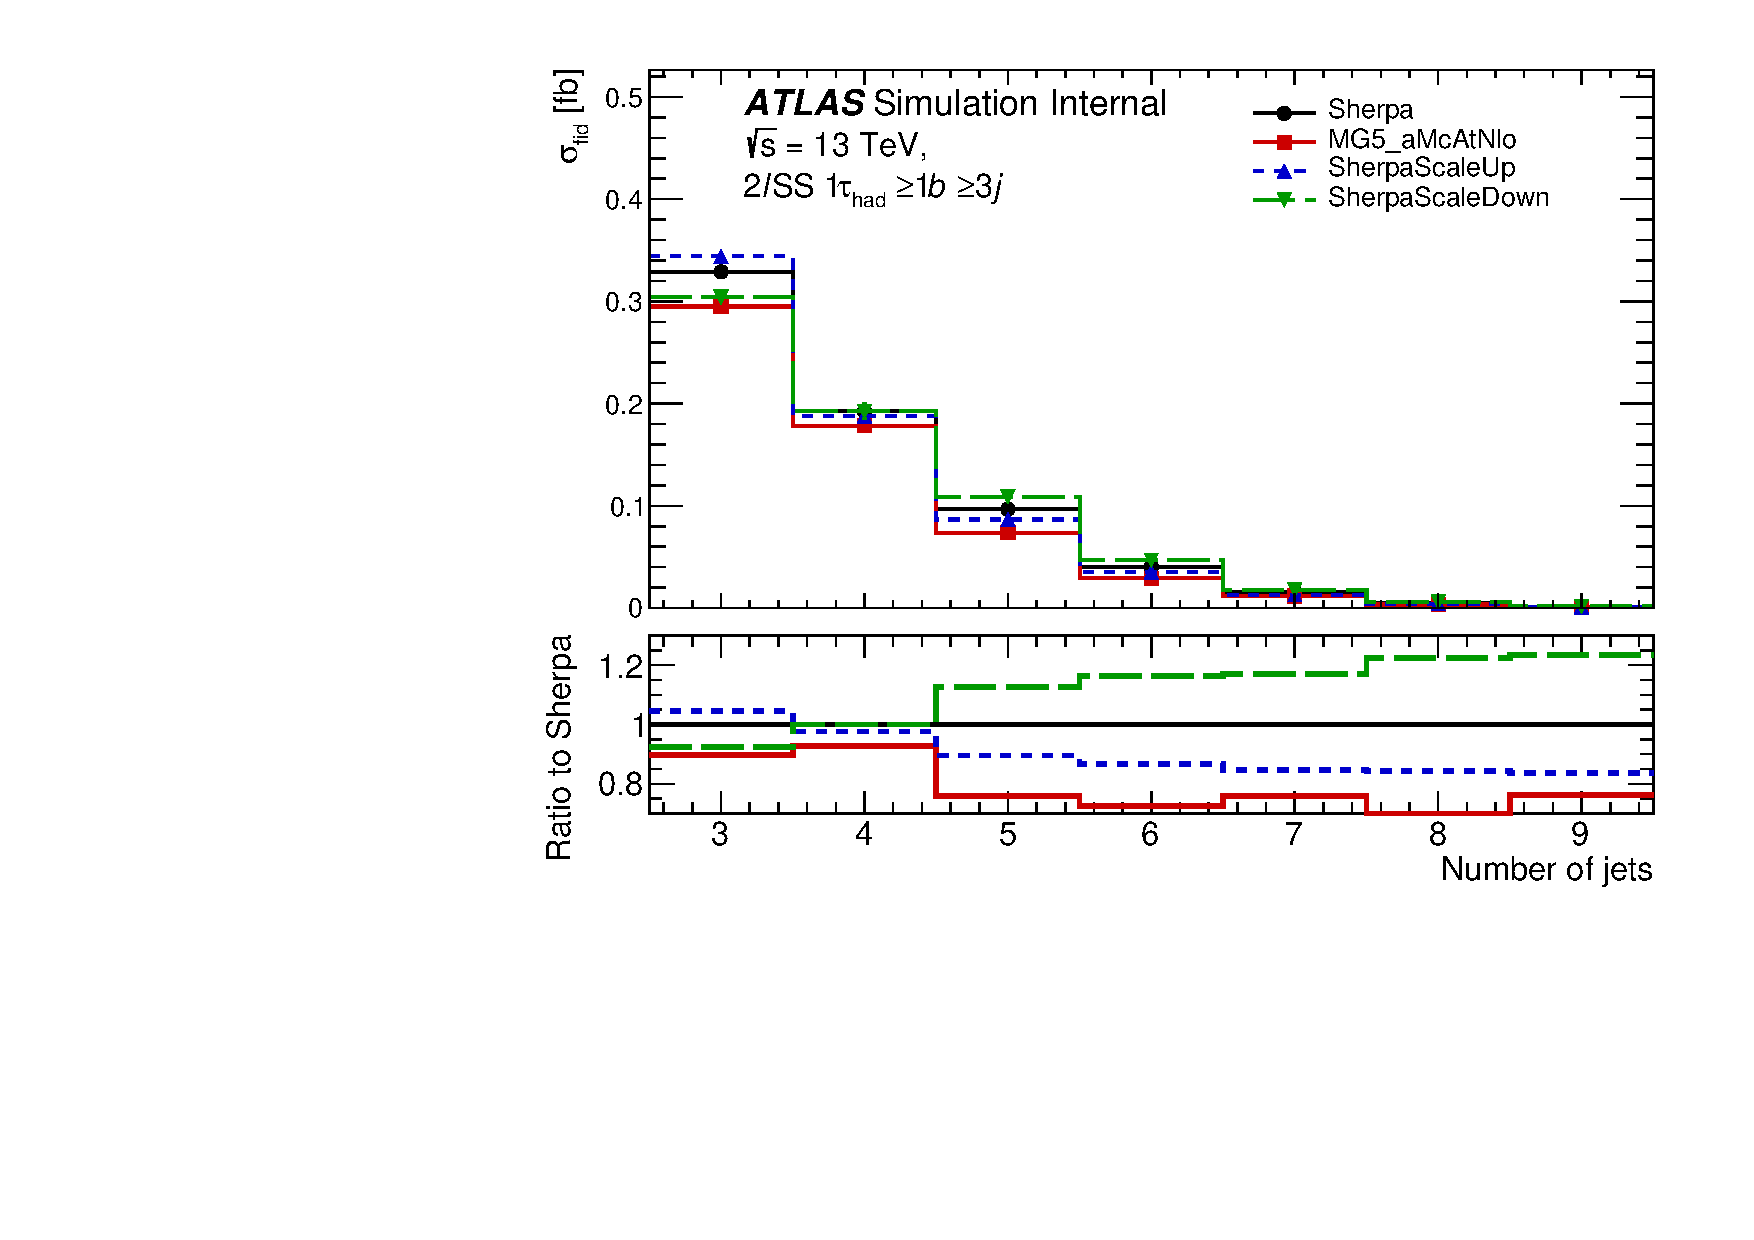
\includegraphics[width=0.45\textwidth]{Plots/ttV/generator/c_Region_4_nJets}
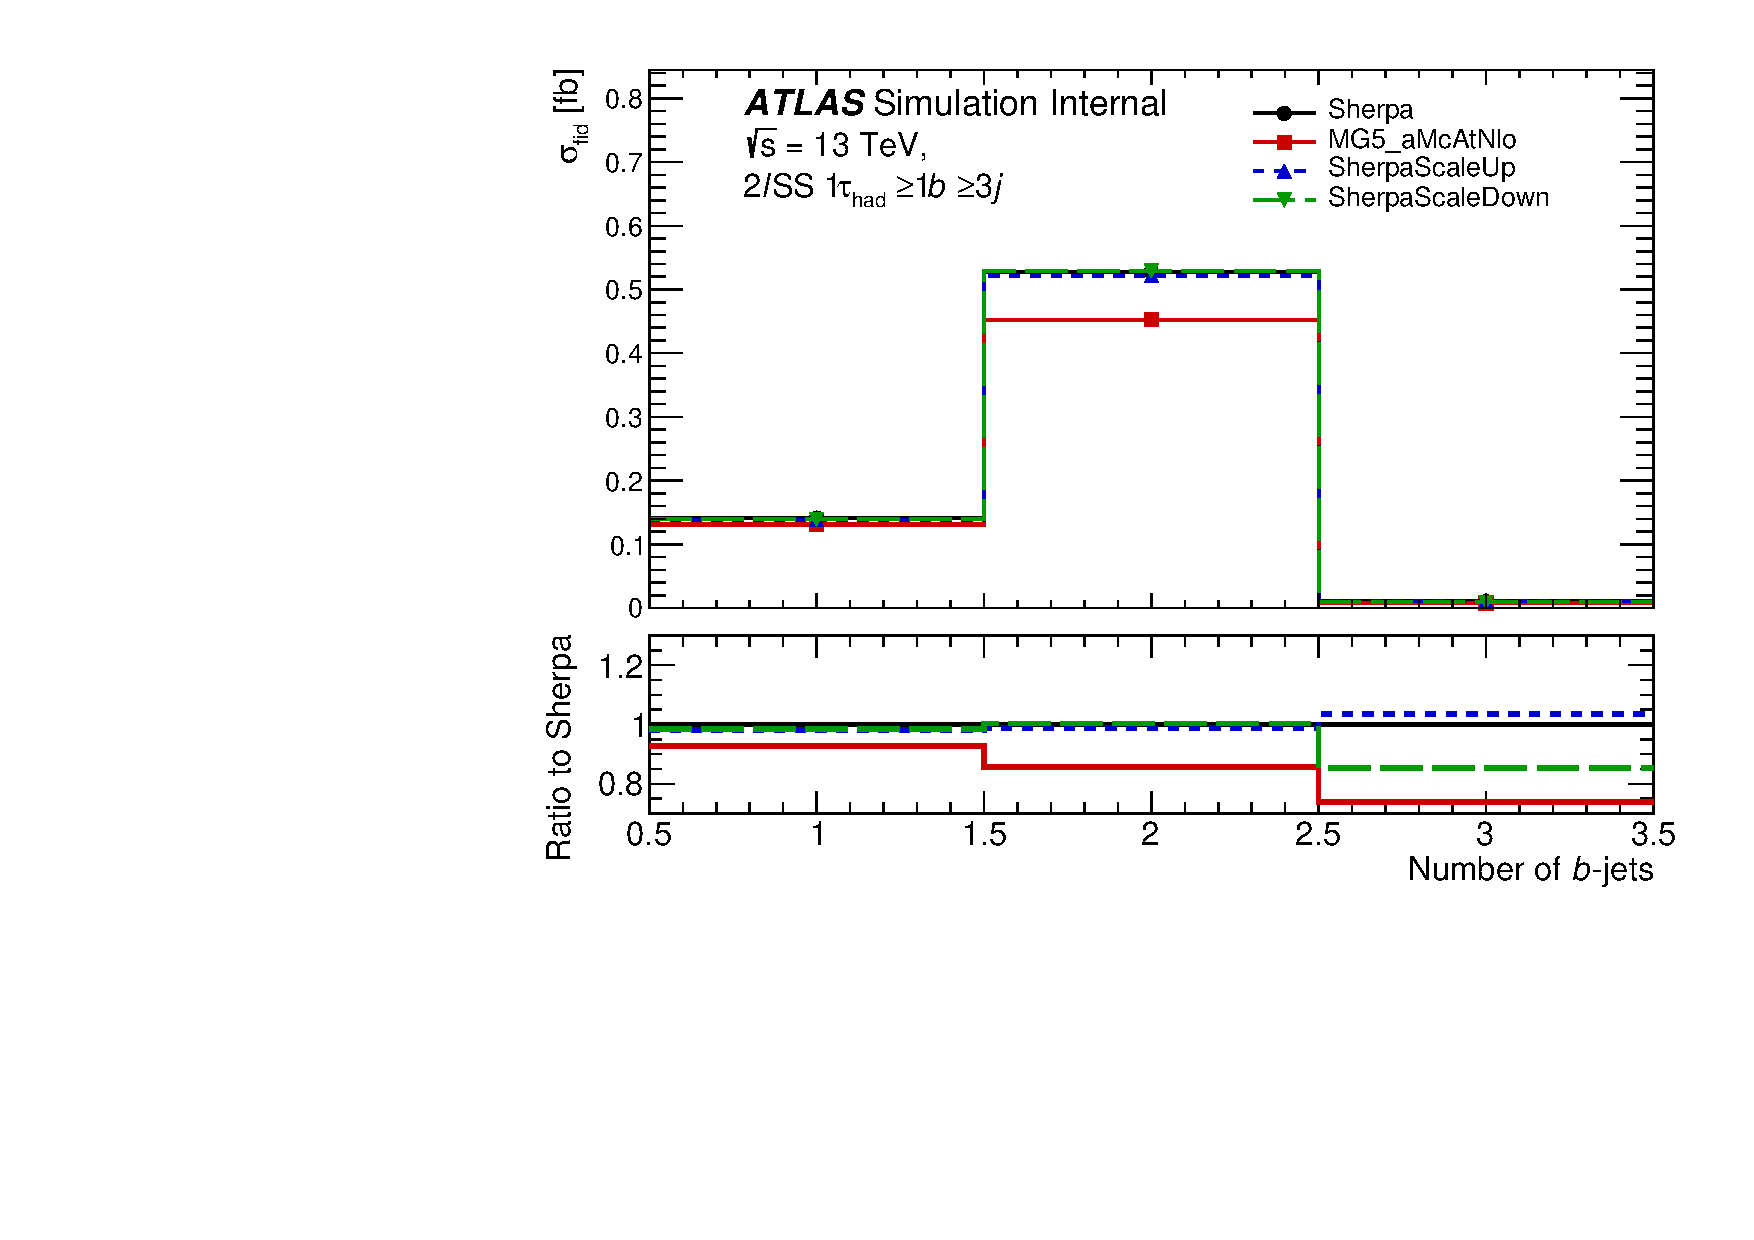
\includegraphics[width=0.45\textwidth]{Plots/ttV/generator/c_Region_4_nBtagJets}\\
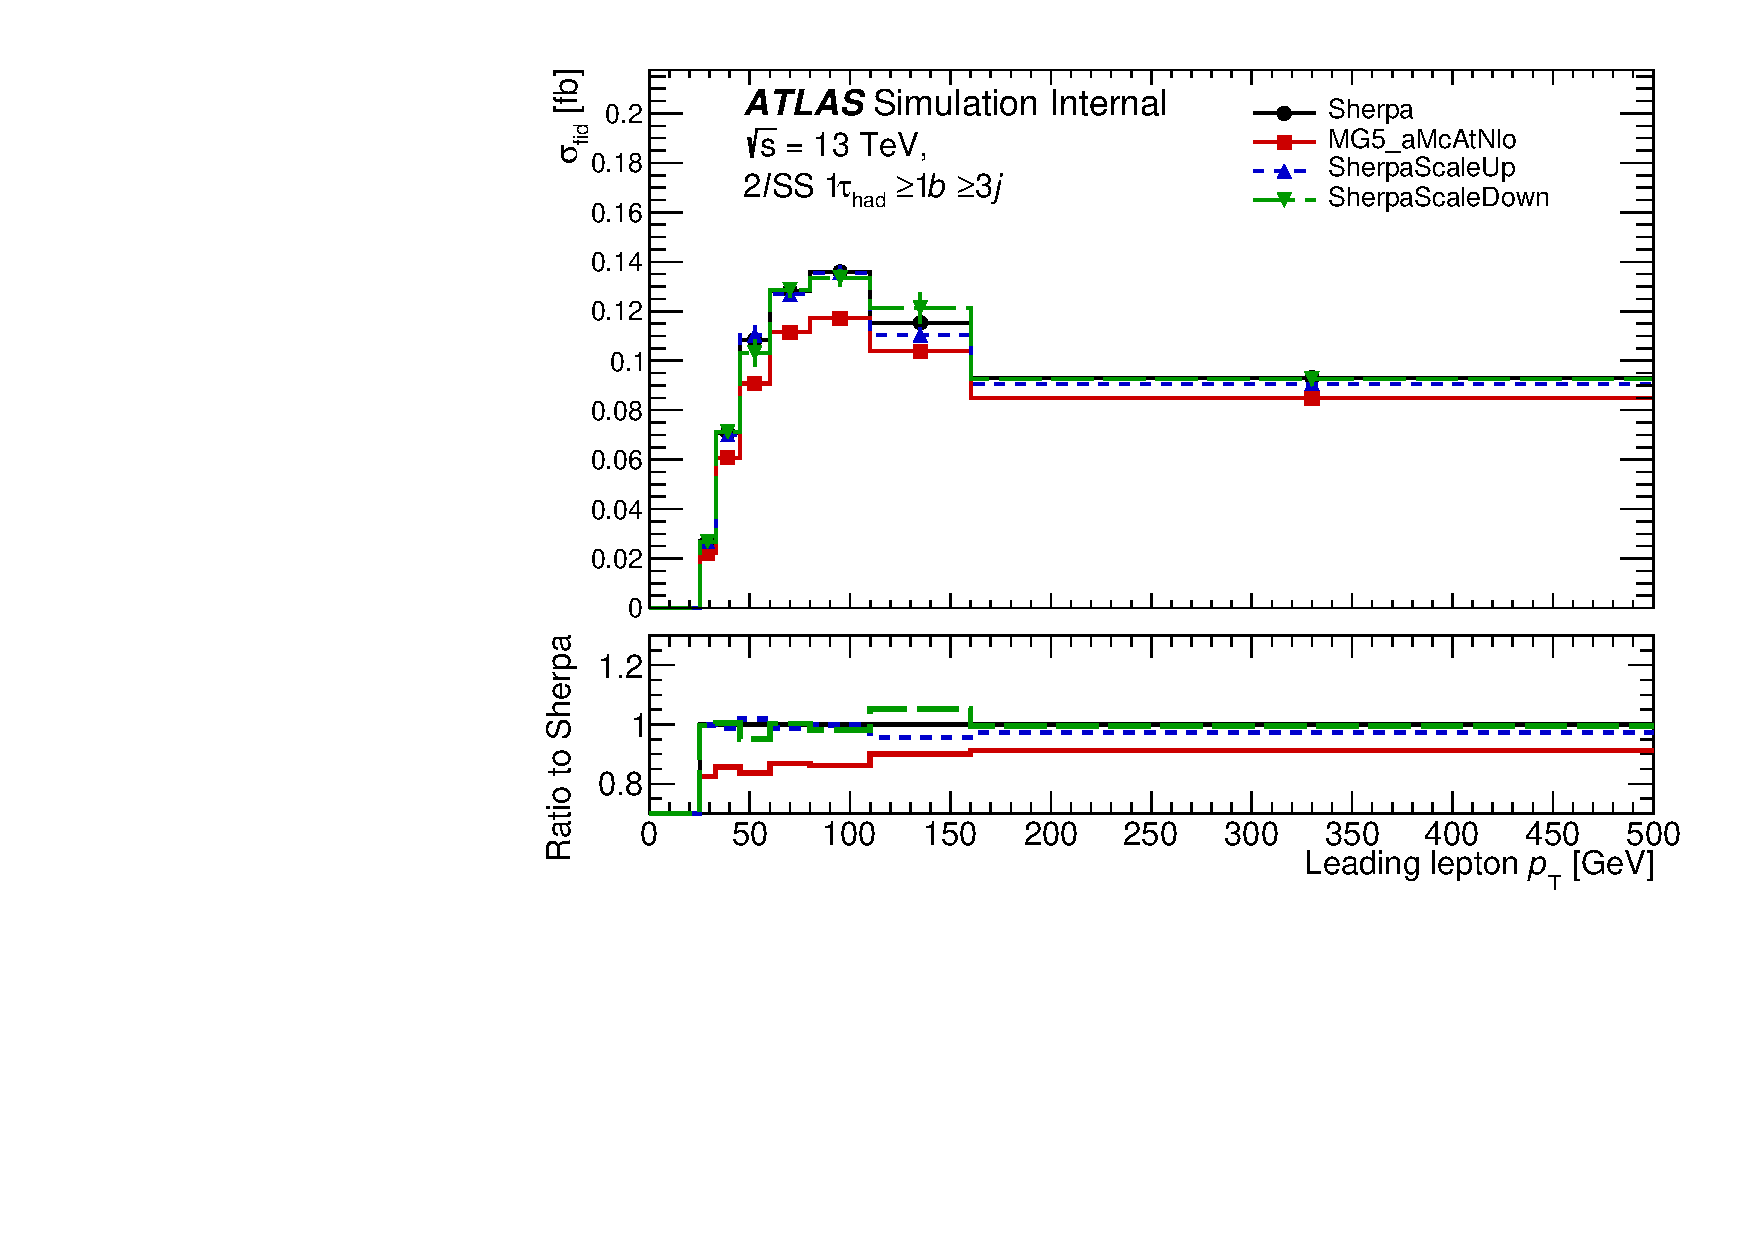
\includegraphics[width=0.45\textwidth]{Plots/ttV/generator/c_Region_4_lep_Pt_0} 
\includegraphics[width=0.45\textwidth]{Plots/ttV/generator/c_Region_4_DRll01}\\
  \caption{Distribution of the the jet multiplicity, number of $b$-jets, the leading lepton transverse momentum and the angular distance between the two leptons  $\Delta R _{\ell \ell }$ for the Region 5 with 1$\tau_{had}$ selection. 
   \label{ttV:den_tauR_kin}}
\end{figure}
% 
